\documentclass[a4paper, man, floatsintext]{apa7}

% Language setting
\usepackage[english]{babel}

% Useful packages
\usepackage{amsmath}
\usepackage{amssymb}
\usepackage{graphicx}
%\usepackage[colorlinks=true, allcolors=blue]{hyperref}
\usepackage[natbib=true,maxcitenames=2,bibstyle=authoryear, style=apa]{biblatex}
\usepackage{csquotes}
\DeclareLanguageMapping{american}{american-apa}
\bibliography{interferencebib}

\usepackage{gb4e}
\usepackage{pifont}
\noautomath
\usepackage{authblk}
\usepackage{rotating}
\usepackage{multirow}
\usepackage{subcaption}

\usepackage{bigdelim}

\usepackage{clipboard}
\newclipboard{output-reviews}
\openclipboard{output-reviews}

\title{\hspace{1cm} Do syntactic and semantic similarity lead to interference effects?
\newline
Evidence from self-paced reading and event-related potentials using German}

\authorsnames[1,{2},1]{Pia Schoknecht, Himanshu Yadav, Shravan Vasishth}
\authorsaffiliations{{Department of Linguistics, University of Potsdam},
{Department of Cognitive Science, Indian Institute of Technology Kanpur}}

  
\shorttitle{Syntactic and semantic interference effects}


\authornote{This research was funded by the Deutsche Forschungsgemeinschaft (DFG, German Research Foundation), Project ID 317633480, SFB 1287.
We thank Johanna Thieke, Romy Leue, Elise Oltrogge and Lisa Plagemann for assistance during data acquisition. We are grateful to Dario Paape for helpful discussions.
Correspondence concerning this article should be addressed to Pia Schoknecht, e-mail: pia.schoknecht@uni-potsdam.de
}

\abstract{Cue-based retrieval accounts of sentence processing postulate that at a verb, retrieval cues are generated to complete a dependency with the verb's argument(s); for example, the dependency between the subject and the verb must be completed to interpret the sentence. If these retrieval cues match with not only the features on the noun that is the retrieval target but also with those on other nouns in the sentence, then processing difficulty arises at the verb. This difficulty in identifying the correct dependent is called similarity-based interference. 
We present large-sample self-paced reading (N = 774) and event-related potentials experiments (N = 103) using a well-established design \citep{vandyke07,mertzen}, to investigate interference due to syntactic and semantic cues in German. 
A Bayes factor analysis showed that both the self-paced reading times as well as event-related potentials provided clear evidence for a semantic interference effect. In the self-paced reading experiment, interference due to the semantic cues caused a reading time slow-down starting at the distractor. 
The event-related potentials showed a more negative N400 amplitude at the critical verb, i.e., the retrieval site, for high vs.\ low semantic interference.
Surprisingly, in both experiments, Bayes factor analyses showed evidence against interference due to syntactic cues. This finding contradicts the predictions of the standard implementations of cue-based retrieval theory, which (implicitly) assume that both syntactic and semantic cues play an equal role in retrieval. We show through computational modeling that cue-based retrieval also shows no syntactic interference if the parser is assumed to keep track of which clause the subject occurs in. Thus, if syntactic retrieval cues include hierarchical syntactic information (is the noun in the same clause as the verb?), the predictions of the cue-based retrieval model would be consistent with the observed patterns in our data. 

In sum, this large-sample study of German using self-paced reading and event-related potentials suggests that, in our data, although both syntactic and semantic cues drive retrieval at the verb, syntactic cues may include hierarchical syntactic information, which can render the parser immune to syntactic interference effects.

\clearpage


}

\begin{document}

\maketitle

\section{Introduction}

\Copy{intro}{It is well-established in sentence processing that completing linguistic dependencies requires memory retrieval \textcolor{blue}{\parencite[see e.g., ][]{lewis06}}. As an example, consider 
(\ref{ex:1_vandyke07}).

\begin{exe}[ht]
\ex \label{ex:1_vandyke07} 
The worker was surprised that the resident who was living near the dangerous warehouse was complaining about the investigation. \parencite{vandyke07}
\end{exe}

There is clear evidence in the literature \parencite[e.g.,][]{jaeger_etal_2020, nicenboim, vandyke_mcelree06, vandyke_lewis03} that, at the verb \textit{was complaining}, it is necessary to retrieve the subject \textit{the resident} from memory in order to interpret who did what to whom. A widely-held assumption is that such memory retrievals during sentence comprehension are guided by retrieval cues \textcolor{blue}{\citep{Lewis2005, mcelree}}.}\label{intro}

Here, we consider two kinds of cues used in retrieval: semantic and  syntactic cues.
In a sentence like (\ref{ex:1_vandyke07}), the retrieval cues generated at the verb are standardly assumed \parencite[e.g.,][]{vandyke07} to include at least the semantic cue \{+animate\} and the syntactic cue \{+grammatical subject\}. These cues pick out the target noun \textit{the resident} as the subject. The distractor \textit{warehouse}, intervening between subject and verb, does not match either of these retrieval cues. However, if the distractor were \textit{neighbor} instead of \textit{warehouse}, then it would match the \{+animate\} cue at the verb. This overlap in cues between the target noun and the distractor is called cue-overload in cue-based retrieval accounts, and is predicted to trigger semantic interference, which expresses itself as greater processing time at the verb compared to the baseline condition (\ref{ex:1_vandyke07}).

By contrast, syntactic interference is expected to be triggered if the distractor matches the \{+grammatical subject\} cue. This situation can occur when the relative clause  in (\ref{ex:1_vandyke07}) that modifies \textit{the resident} were to be changed to \textit{who said that the warehouse was dangerous}. Now, the distractor matches the \{+grammatical subject\} cue.

Thus, a distractor which matches a semantic cue, here, \{+animate\}, is predicted to induce semantic interference and a distractor which matches a syntactic cue, here, \{+grammatical subject\}, is predicted to induce syntactic interference. More generally, interference that is induced by such an overlap between retrieval cues and features of items in memory is called retrieval interference.

Previous work has shown clear evidence for this kind of retrieval interference \parencite{vandyke07, vandyke_mcelree06, vandyke_mcelree2011, nicenboim,  vandyke_lewis03,jaeger_etal_2017}. However, two important questions remain unanswered. First, as discussed in \textcite{jaeger_etal_2017}, almost all the published studies on interference effects are severely underpowered. Low power has the consequence that published estimates will tend to be overestimates or misestimates of the effect size \parencite{vasishth2018_signficancefilter}. Over-/misestimates have important implications for theory evaluation. One example is discussed in \textcite{vasishth2018_signficancefilter}, where a key prediction of surprisal theory \parencite{levy&keller_2013} could not be validated when a larger-sample study was conducted. By contrast, the original small-sample study \parencite{levy&keller_2013} showed suggestive evidence consistent with the theory. Another example is the recent heated debate \parencite{nieuwland_etal_2018} on prediction in sentence comprehension, which was largely focused on the results of low-powered studies, leading to potentially misleading conclusions \parencite{nicenboim_etal_2020}.
Second, although it has been established \parencite[e.g.,][]{vandyke07,mertzen} that syntactic and semantic cues are involved in sentence processing, it is not obvious which cues are relevant for a particular retrieval event. For example, \textcite{dillon2013} argued, following \textcite{Sturt2003}, that the gender cue was either downweighted or not used at all when an antecedent-reflexive dependency needs to be built. Instead, the antecedent of a reflexive could be identified using the syntactic principle A of the binding theory, which correctly identifies the target for retrieval.  Using computational modeling, \textcite{dillon2013} suggested that antecedent-reflexive dependencies were immune to interference, and that the reason for this is that principle A of the binding theory is the primary driver of the cue-based retrieval process \parencite[cf. ][]{jaeger_etal_2020,yadav2021individual}. This was a surprising discovery because the default assumption in cue-based retrieval accounts was that all cues were equally weighted, regardless of the dependency type; this had the consequence that retrieval interference was expected whenever a cue-overload configuration was present in a sentence. More broadly, an important insight in the work of \textcite{dillon2013}, among others, is that  the precise details of which cues are used during retrieval can affect processing difficulty in possibly surprising ways. We build on this idea in the present paper.

\section{The present study}

Reading studies have been the dominant method used to investigate retrieval interference \parencite[see the review in][]{jaeger_etal_2017}. We aimed to investigate the role of syntactic and semantic cues during sentence comprehension with higher-powered experiments using  self-paced reading (SPR) as well as electroencephalography (EEG), which to our knowledge has never been used to investigate interference during subject-verb dependency resolution.

\Copy{vd_design}{All experiments used the 2 $\times$ 2 design developed by \textcite{vandyke07}; the design crosses syntactic and semantic interference.} \label{vd_design}

\subsection{Materials}

As the same materials were used for all our experiments, we describe them here once before we describe the specifics of the experiments, separately. The studies had 120 items with four conditions in a Latin square design shown in (\ref{ex:materials}). The items were constructed following \citeauthor{vandyke07}'s (\citeyear{vandyke07}) items and partially re-used  \citeauthor{mertzen}'s (\citeyear{mertzen}) items.

\begin{exe}  
\ex \label{ex:materials} Example item (critical word in bold, distractor in italics) of the present study:
    \begin{xlist}   
    \ex {High syntactic interference with high / low semantic interference:}\label{ex:hisyn} 
    \gll Die  Nachbarin glaubte,	dass	der Witwer,  der  erzählt hatte, dass der \textit{Einbrecher} / \textit{Verlust}  schrecklich war, abends regelmäßig \textbf{trank}, um zu vergessen.\\ 
    The\textsubscript{\sc{fem}} neighbor\textsubscript{\sc{fem}} believed that the widower who told had that the burglar / loss awful was in.the.evening regularly drank in.order to forget \\
    \trans `The neighbor believed that the widower, who had told her that the loss was awful, drank regularly in the evenings to forget.' \\
    
    \ex {Low syntactic interference with high / low semantic interference:}\label{ex:losyn} 
    \gll Die  Nachbarin glaubte, dass der Witwer,  der  von    dem schrecklichen \textit{Einbrecher} / \textit{Verlust} erzählt hatte, abends regelmäßig \textbf{trank}, um zu vergessen. \\ 
    The\textsubscript{\sc{fem}} neighbor\textsubscript{\sc{fem}} believed that the widower who about the awful burglar / loss told had in.the.evening regularly drank in.order to forget\\
    \trans `The neighbor believed that the widower, who had told her about the awful loss, drank regularly in the evenings to forget.'  \\
    \end{xlist}
\end{exe}

The comprehension of the sentences in (\ref{ex:materials}) requires a memory retrieval operation at the verb \textit{trank} (`drank') to retrieve its non-adjacent subject \textit{Witwer} (`widower'). During this retrieval, the distractor \textit{Einbrecher} (`burglar') / \textit{Verlust} (`loss') might cause interference and impede comprehension. 

Syntactic interference is manipulated via the syntactic status of the distractor, which is either the subject (\ref{ex:hisyn}) of an embedded clause, or part of a prepositional phrase (\ref{ex:losyn}) and hence a non-subject. \Copy{franck_refs}{Following \textcite{vandyke07}, the assumption here is that  during the retrieval of the subject, a distractor in \emph{any} subject position causes more syntactic interference than a distractor inside a prepositional phrase \textcolor{blue}{ -- even if the distractor occurs in an embedded clause {\parencite[this assumption stands in contrast to findings on so-called agreement attraction, where syntactic hierarchy plays a crucial role, see e.g.,][]{franck2002subject, franck2006agreement,franck2011_commentary, franck2020hierarchical}.}}}\label{franck_refs}

Semantic interference is manipulated via the animacy of the distractor. During the retrieval of the subject of the verb \textit{trank} (`drank'), the animate distractor  \textit{Einbrecher} (`burglar') is assumed to cause high semantic interference, while the inanimate distractor \textit{Verlust} (`loss') is assumed to cause low semantic interference. \Copy{semantic_features_encoding}{\textcolor{blue}{The animacy of the distractor is used as a stand-in feature for semantic features relevant for the specific retrieval event which might be more fine-grained. In \ref{ex:materials}, the semantic retrieval cue might be \{+animate\} or \{+human\} but it might as well be \{+can drink\}. While more generic features like \{+animate\} or \{+human\} (all animate distractors were human) might be created during memory encoding, more specific features like \{+can drink\} are probably only activated when relevant. The present study is not designed to provide insight into the specific semantic features used during memory encoding and retrieval (for work on highly specific retrieval cues like \{+sailable\} and \{+shatterable\}, see \cite{vandyke_mcelree06, cunnings_sturt_2018retrieval}). A plausibility norming experiment (see page \pageref{plausib_normin_orig}) was conducted to ensure that the semantic manipulation did work, i.e., that the semantic requirements of the verb matched the features of the subject and the animate distractor, but not the features of the inanimate distractor.
}}\label{semantic_features_encoding}

\paragraph{Regions of interest in the design}
\textcolor{blue}{For both our SPR and EEG experiments, o}ur principal focus was on the processing of the verb (\textit{trank}, `drank'). \textcolor{blue}{In the SPR experiment, t}he reading times of the immediately following spill-over region and of the pre-critical region were also of interest. Previous work using the present design \parencite{vandyke07,mertzen} has consistently found effects in the pre-critical region (we return to this point in the discussion sections\textcolor{blue}{, see Figure \ref{fig:previous_vs_present} A}). A further issue with German embedded clauses \parencite[also see][]{mertzen} was that, without an appropriate intervening phrase, the clause embedding would lead to two verbs appearing one after another (\textit{erzählt hatte, trank}, literally `told, drank'). This is because in German, the verb is clause-final in embedded clauses. Such verb sequences are inherently difficult to process \parencite{VSLK11,bach1986crossed}. 

For these reasons, we added two adverbs before the critical verb. Including these intervening regions had a further advantage: 
It is well-known \parencite[e.g., ][]{rayner2000effect} that the last word in a clause-final position causes a slowdown in reading; such a slowdown has the potential to spill over to the subsequent regions, possibly affecting the estimated effects at the critical region. The spill-over of longer reading times can be problematic because the standard deviation increases as well \parencite{wagenmakers2007linear}; such an increase in standard deviation would drastically lower statistical power. 
Inserting two adverbs before the critical verb thus served to attenuate spill-over from the clause-final word in the embedded clause preceding the critical region. This way, the critical region should be less affected by the clause-boundary slowdown. This design also has the advantage that any potential effects seen at the pre-critical region (the adverb immediately preceding the verb) are less likely to be due to spill-over from the preceding region. Thus, our focus in the \textcolor{blue}{SPR experiment} is on the processing difficulty observed at the critical verb and the surrounding regions.

\Copy{why_n400}{\textcolor{blue}{In the EEG experiment, the region of interest is the critical verb. Due to the direct measurement of brain activity with excellent temporal resolution event-related potential (ERP) effects do not tend to spill-over into later regions. We focus specifically on the N400 elicited by the verb. The N400 is a negative deflection in the ERP signal that peaks approximately 400 ms after any word was encountered. Traditionally, it is associated with lexical-semantic processing, but the finding of multi-modal N400 effects suggests that it rather indexes differences in the processing of meaningful stimuli in general \citep{kutas_federmeier2011}. The N400 amplitude is greater for words that deviate from the meaning activated by its context compared to words that fit its context \citep[see e.g.,][]{kutas_hillyard, Kutas_Iragui_1998}. Consequently, the amplitude of the N400 to a specific word is a negative function of its predictability within the given context \citep[see e.g.,][]{kutas_hillyard1984, frank2015_erp_surprisal}. Additionally, the N400 elicited by isolated words is negatively correlated with their frequency \citep{kutas&federmeier_2000}. Therefore, the N400 amplitude is thought to index a) the increased difficulty to integrate a semantically anomalous or simply unexpected word into the sentence context \citep[e.g.,][]{hagoort2004integration} and/or b) the necessity to retrieve lexical information from memory which was not already pre-activated before the stimulus was perceived \citep[e.g.,][]{brouwer2017_n4_p6}. These two accounts of the N400 have been extensively discussed in the ERP literature on prediction \citep[see e.g.,][]{nieuwland_etal_2018, nicenboim_etal_2020, Freunberger_Roehm_2017, Delong_etal_2005, mantegna2019, nieuwland2019_integrationprediction}. As a likely marker of memory retrieval during sentence comprehension, it is fair to assume that the N400 would show modulations due to retrieval interference. The few ERP studies that have investigated retrieval interference so far have indeed found negativities \citep{lee_garnsey, martinetal2014, schoknecht2022, vasishth_drenhaus_2011}, although the topography and latency of these negativities was mostly not typical for the N400. It is important to highlight here that the previous ERP studies on interference either increased the number of distractors in a sentences or used grammatical gender or number as the critical retrieval cue. So, interference due to non-semantic features elicited negativities which were more or less similiar to the N400. Therefore, we expect the interference manipulation regardless of the type of retrieval cue (syntactic or semantic) to elicit N400 or similar effects. For a discussion of the relation between the N400 and other negativities, see \textcite{ina_n400}.}

\textcolor{blue}{Alternately, retrieval interference -- especially syntactic retrieval interference -- might modulate the P600. The P600 is a positive deflection in the ERP wave form that is typically observed at least 600 ms after stimulus onset. It is associated with syntactic processing, e.g., morpho-syntactic errors and reanalysis \citep[see, e.g.,][]{osterhout&holcomb_1992, kaan_etal_2000_P600}. High interference could increase difficulty during syntactic integration of subject and verb in our materials. Potential misretrievals of the distractor might lead to reanalysis which could manifest as an increased P600 amplitude in high compared to low interference conditions.}} \label{why_n400}




\subsubsection{Plausibility norming} \label{plausib_normin_orig}
\citeauthor{vandyke07} conducted a pre-test to ensure that the distractor in high semantic interference conditions was a sufficiently probable subject of the critical verb, i.e., that it could potentially induce semantic interference. Following \citeauthor{vandyke07}, we also conducted a plausibility norming experiment.

\paragraph{Participants in the plausibility norming study}
Forty participants (18 female, 22 male, mean age: 27.3 years old, age range: 21 - 39 years old) from the SPR experiments were re-invited for the plausibility norming one month after they completed the SPR experiment. We used a subset of the participants who participated in the SPR study in order to ensure that the ratings for the norming came from the same pool of participants that did the reading study.

\paragraph{Materials in the plausibility study}
For each of the 120 item quadruplets, four simple sentences with subject-verb-object word order were constructed, so that each of the nouns in the item once functioned as the subject of the critical verb. The norming materials corresponding to the item depicted in (\ref{ex:materials}) are shown in (\ref{ex:materials_norming}).

\begin{exe}  
\ex \label{ex:materials_norming}
    \begin{xlist}   
    \ex {Subject}:\label{ex:subject} 
    \gll Der Witwer trank. \\ 
    the widower drank\\
    \trans  `The widower drank.'\\  
    \ex {Animate distractor:}\label{ex:animate_dist} 
    \gll Der Einbrecher trank. \\ 
    the burglar drank \\
    \trans `The burglar drank.' \\
   \ex {Inanimate distractor:}\label{ex:inanimate_dist} 
    \gll Der Verlust trank.  \\ 
    the loss drank\\
    \trans  `The loss drank.'\\  
    \ex {Introduction noun:}\label{ex:intro_noun} 
    \gll Die Nachbarin trank.\\ 
    the\textsubscript{\sc{fem}} neighbor\textsubscript{\sc{fem}} drank \\
    \trans `The neighbor drank.' \\
    \end{xlist}
\end{exe}

Thus, each of the forty participants were asked to rate $120 \times 4$ sentences, leading to 19,200 data points.

\paragraph{Procedure for the plausibility study}
The plausibility norming experiment was implemented in PCIbex \citep{pcibex} and was conducted online. Participants were asked to judge the plausibility of the sentences on a 7-point scale ranging from absolutely implausible (1) to absolutely plausible (7). All sentences belonging to one item were shown on one screen, so that they could be judged relative to each other. The plausibility norming experiment included 120 sentences from a different experiment which functioned as fillers. The participants received \pounds 3.40 as compensation for the norming experiment. A demonstration of the plausibility norming experiment can be accessed via \hyperlink{https://farm.pcibex.net/r/WIeKYM/}{https://farm.pcibex.net/r/WIeKYM/}.

\paragraph{Results of the plausibility study}
The plausibility ratings showed that the semantic manipulation worked as intended. The subject received the highest rating (mean: 6.5, sd: 0.9) and the animate distractor (high semantic interference conditions) was almost as plausible (mean: 6.1, sd: 1.3). In contrast, the inanimate distractor (low semantic interference conditions) was very implausible (mean: 1.7, sd: 1.4). The first noun in the target sentences, which was not part of the experimental manipulation, was tested as well and it received a high plausibility rating (mean: 6.0, sd: 1.4). These results are shown in Figure \ref{fig:plausibility_rating}. The plausibility ratings are similar to those reported for \citeauthor{vandyke07}'s (\citeyear{vandyke07}) Experiment 3.

\begin{figure}[H]
\caption{Plausibility ratings for the animate (high semantic interference conditions) and inanimate distractor (low semantic interference conditions), the introduction noun (\textit{X believed that \dots}) and the subject. The diamonds represent the mean rating. Blue dots show the individual data points. }\label{fig:plausibility_rating}
\centering
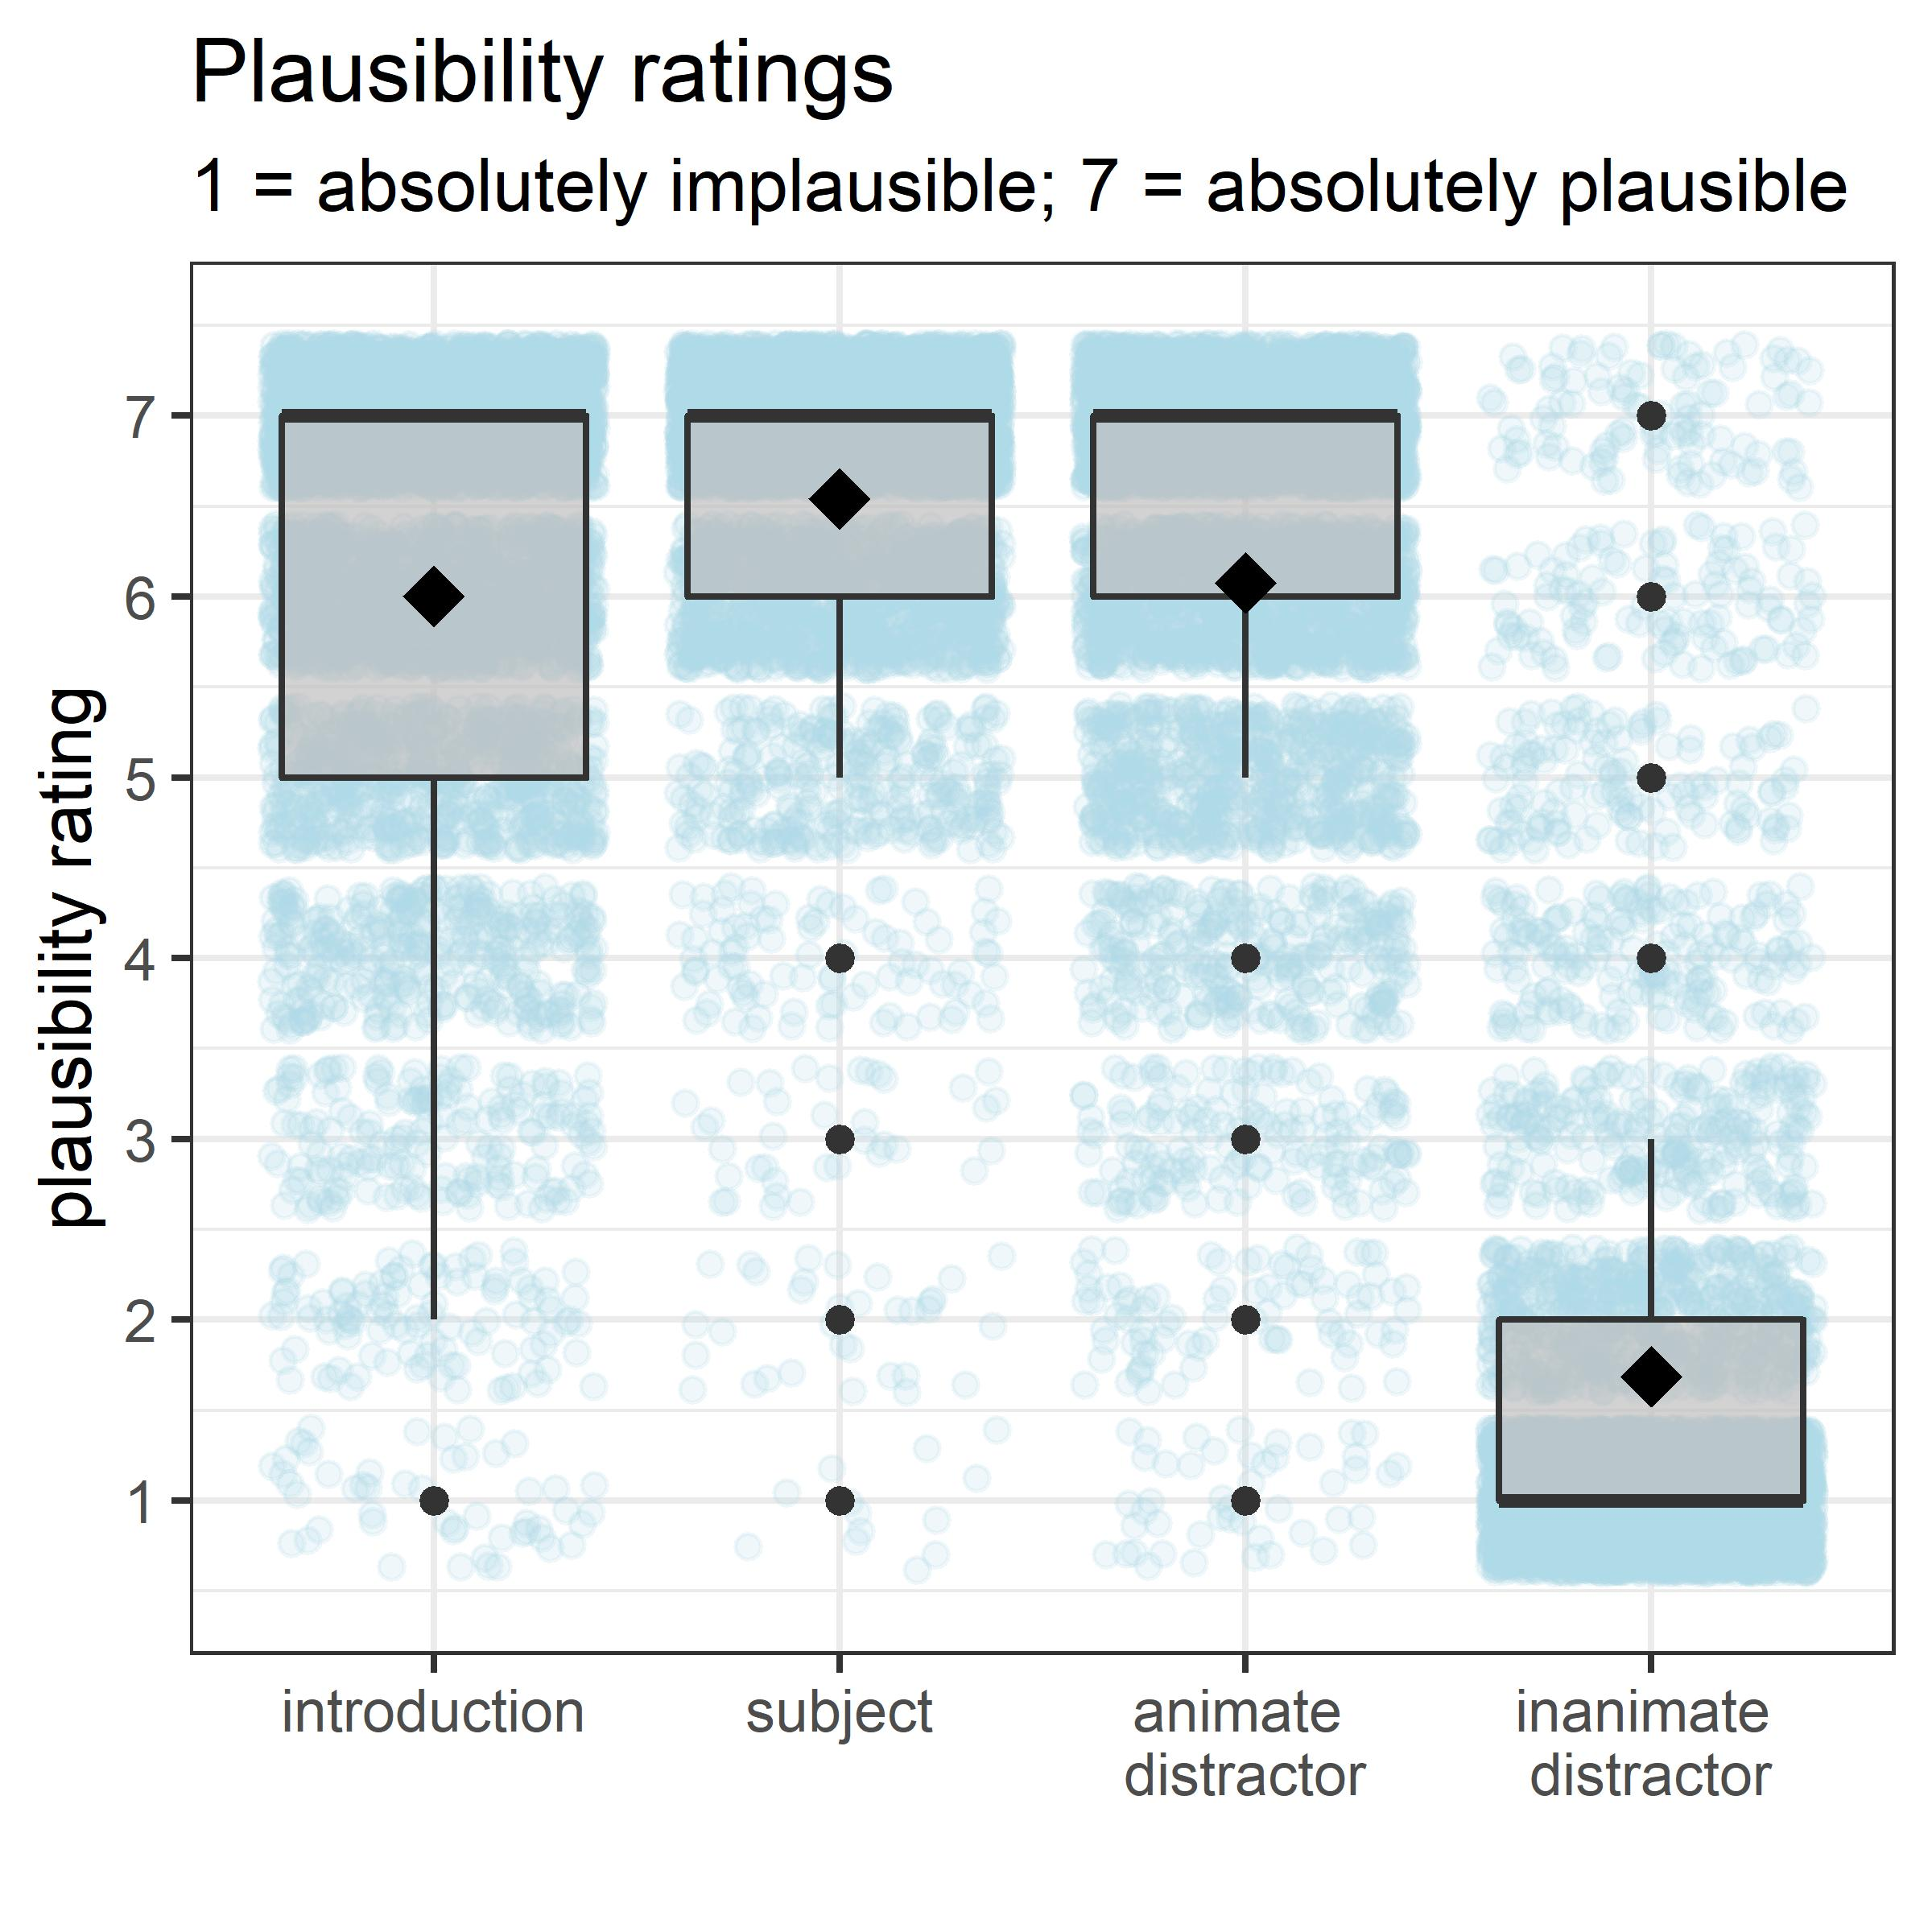
\includegraphics[width=0.6\textwidth]{images/pandora_plausibility_ratings.jpg}
\end{figure}


\subsection{The structure and sample sizes of the SPR and EEG experiments}

The SPR experiments were conducted web-based via Prolific and the EEG experiment was of course run in the lab.  Because the signal-to-noise ratio of EEG data requires a large number of trials per condition and participant, we constructed 120 items. In order to keep the SPR and EEG studies comparable, we also used 120 items in the SPR experiments. In both methods, as it would have been very taxing for the participants to read all 120 items in one experimental session, we split the experiments into two sessions. 

The SPR study, hereafter Experiment 1a, was initially designed so that participants read items in the first session (1-60) and then, after a gap of 1-20 days, they read the the second set of items (61-120). The variation in the gap is due to the fact that we could not control when the participants would do the second session; however, the mean and median gaps were  about 11 days, with the first and third quartiles being 9 and 12 days.

As discussed in detail below, the second session showed an adaptation effect \parencite{prasad2021rapid}: Reading times decreased overall. The adaptation effect is theoretically interesting per se \parencite{fine2013rapid} and we discuss it below; but it was problematic for our design because the average effect would then be confounded by adaptation. For this reason, we ran a second version of the SPR study, hereafter Experiment 1b, in which participants (N=570) were either shown items 1-60 or items 61-120 (but not both). In the Results section, we present both sets of results as well as the pooled data (N=774) from E1a and E1b.
As mentioned above, because the ERP method requires a large number of items, all the ERP data come from participants who completed both sessions. 

Figure \ref{fig:project_str} shows the structure of the present study, i.e., how many participants saw which subset of the items and whether these participants completed one or two experimental sessions.

\begin{figure}[H]
    \caption{The structure of the present study. In total, 120 items were used for the SPR (red branches) and the ERP experiments (blue branches). The color brightness reflects how many sessions were completed by each participant (lighter color: two sessions, darker color: one session).}
    \label{fig:project_str}
    \centering
    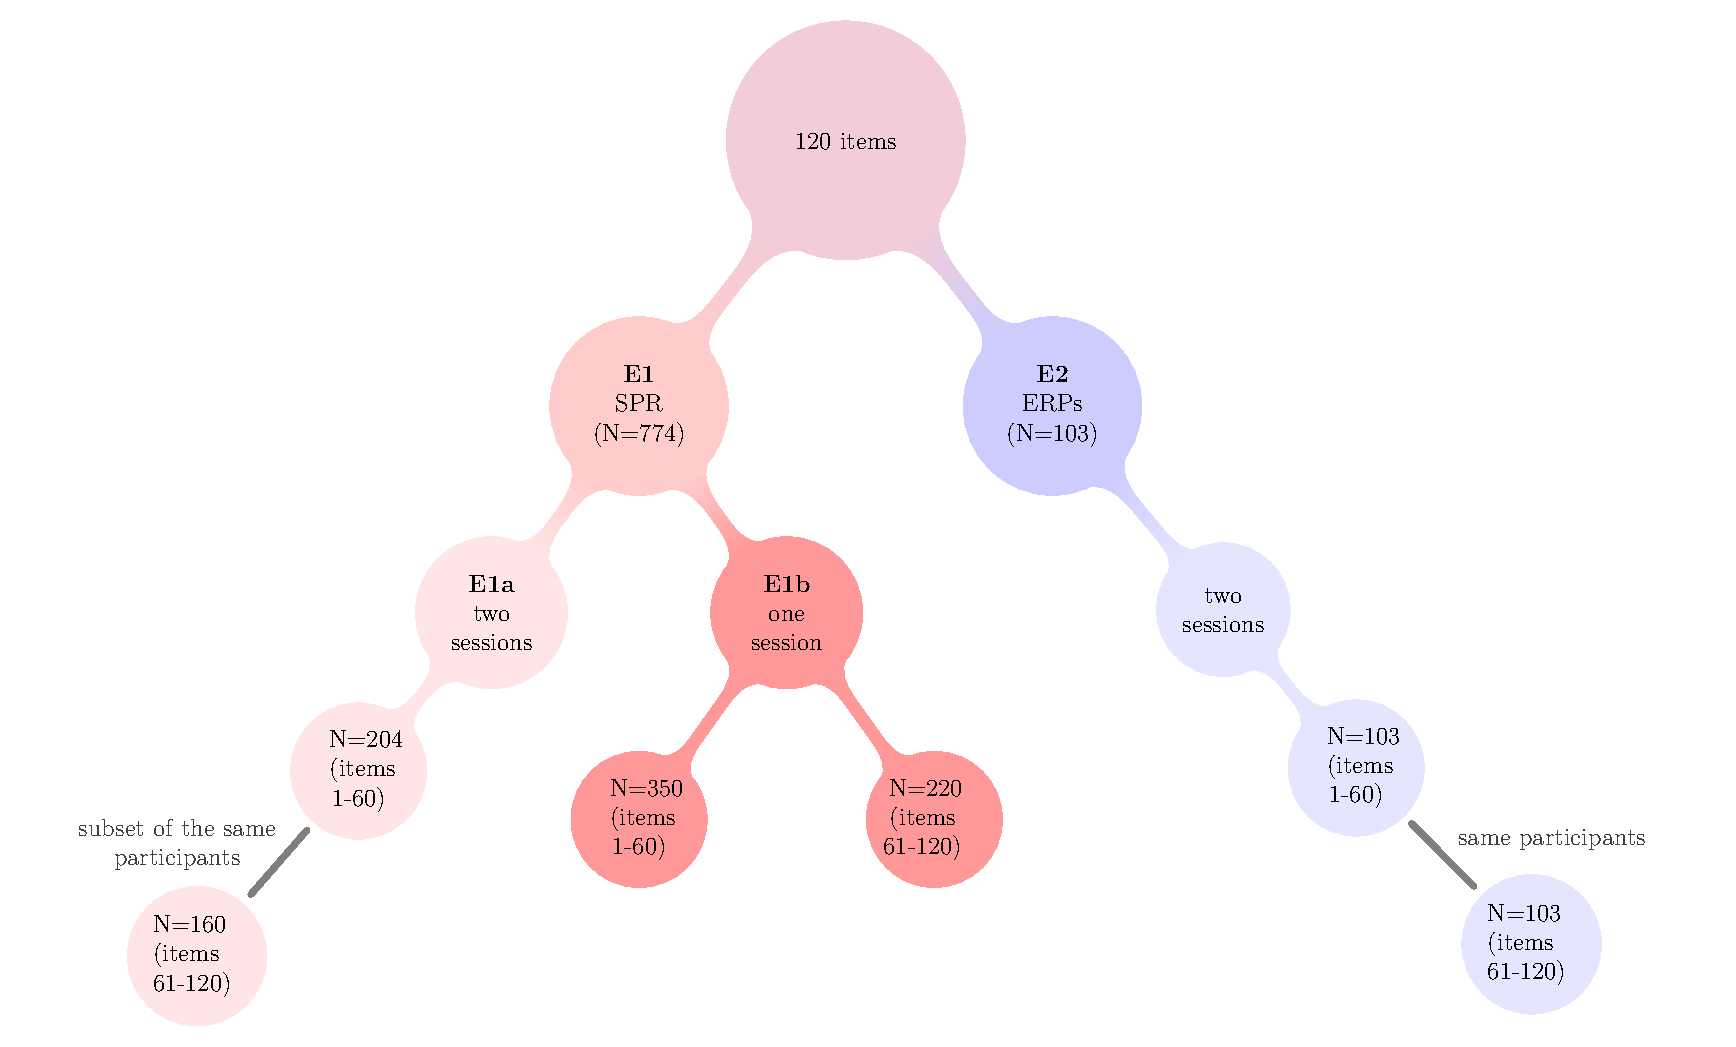
\includegraphics[width=\textwidth]{images/pandora_project_structure_figure.pdf}
\end{figure}

\Copy{osf}{\textcolor{blue}{\section{Data availability statement}
All materials, data and analysis scripts can be accessed via https://osf.io/4fpru/?view$\_$only=2d2a004d3e4147bc975b5e8c455c27df.}}\label{statement}


\section{Experiments 1a and 1b: SPR}

\subsection{Methods}
\subsubsection{Participants}

Native German-speaking participants were recruited via Prolific. In total, 908 participants took part in the self-paced reading experiments E1a and E1b. 117 participants were excluded due to low comprehension question accuracy (< 70\,\%). Additionally, 16 participants were excluded because the demographic information in their Prolific profile and the information which they provided during the experiment did not match (regarding, e.g., their native language, language impairment, or age). One participant was excluded because of a technical error during their session. The data of 774 participants (mean age: 27 years old, age range: 18 - 40 years, 395 female, 369 male, 10 preferred to not provide sex information) were used for analyses. When asked about their highest level of education, 365 participants reported a bachelor's degree or higher university education. 334 participants reported to have a high-school diploma and 70 another secondary school certificate. Five participants replied with ``other.'' 

In Experiment 1a, drop-outs between sessions led to a lower sample size in the second session (204 vs.\ 160). In Experiment 1a, compensation for the first session was \pounds 3.5 and for the second session, it was \pounds 5. In Experiment 1b, compensation was \pounds 4. 

\subsubsection{Procedure}
Participants completed a moving window self-paced reading task \citep{just_etal_1982} on the PCIbex Farm \citep{pcibex}. They were instructed to read for comprehension at a comfortable pace. All sentences were displayed word by word. Masked words were presented as a line indicating its length. Unmasked words were presented in 18 pt Courier font. The space bar on the keyboard was used to unmask words. The length of the sentences required line breaks. These were hard-coded so that in each sentence a line break appeared i) between the subject and the relative clause and ii) two words after the critical verb (see \ref{ex:linebreak}, critical word in bold, | indicate line breaks in the moving window display). In a third of the trials, the sentence was followed by a yes/no comprehension question. The participants received no feedback on their performance.

In addition to the reading-for-comprehension task, the participants completed two types of attention and compliance checks. The attention checks required them to press one of two designated keyboard keys ten times during each session. The compliance checks required them to type in two types of fruit and two hobbies (session 1) and two German cities and two breakfast food items (session 2). No participant failed any of these checks. The reader can try the experiment via this link \hyperlink{https://farm.pcibex.net/r/CBkSKl/}{https://farm.pcibex.net/r/CBkSKl/}. 

\begin{exe}  
\ex \label{ex:linebreak}
    \gll Die Nachbarin glaubte, dass der Witwer, | der erzählt hatte, dass der Verlust schrecklich war, regelmäßig abends \textbf{trank}, um zu | vergessen. \\ 
    The neighbor believed that the widower | who told had that the loss awful was regularly in.the.evening drank in.order to | forget\\
    \trans  `The neighbor believed that the widower, who had told her that the loss was awful, regularly drank in the evenings to forget.'\\  
\end{exe}

\Copy{fillers1}{In Experiment 1a, participants were re-invited for session 2 after they completed session 1. The experimental sessions were separated by 1 - 20 days. The procedure of the sessions was identical. \textcolor{blue}{In session 1, the experimental items 1-60 were presented interspersed with 40 filler sentences. In session 2, the experimental items 61-120 were presented with another set of 40 filler sentences. The fillers were less syntactically complex than the experimental items but had at least one embedded clause and generally provided more variety (e.g., ``Der Teppichmacher, der früh in die Werkstatt gekommen war, reparierte den besonders schönen, alten Teppich während er die Nachrichten hörte'', `The carpet maker who came to the workshop early repaired the especially beautiful old carpet while listening to the news.'; ``Der Jugendliche war genervt, weil seine Freundin, die nicht studieren wollte, oft die Schule schwänzte, um Computer zu spielen.'', `The teenager was annoyed because his girlfriend who did not want to go to University  skipped school frequently to play video games.').}}\label{fillers1} Each session lasted approximately 25 minutes.

\subsubsection{Statistical analyses}

\paragraph{Bayesian linear mixed models}
Comprehension question accuracy was analyzed with Bayesian generalized linear mixed models, i.e., logistic regression, in R \citep{r}, using the brms package \citep{brms}. The fixed effects were syntactic interference, semantic interference and their interaction. These were sum-contrast coded (high +0.5, low -0.5). Varying intercepts for participants and items were included. For the intercept, we used a Normal(0, 1.5) prior and  for all fixed-effect slope parameters, a Normal(0, 0.1) prior. The priors for the variance components were the defaults specified in brms. Models were run with 4 chains and 8,000 iterations in each chain. 2,000 iterations in each chain consisted of a warm-up phase. 

Self-paced reading times were analyzed with Bayesian linear mixed models in R \citep{r} with log-normal likelihood, using the brms package \citep{brms}. The critical word for analyses was the verb \textit{trank} `drank' in (\ref{ex:materials}), constituting the retrieval site. Because previous work found effects in the pre-critical and post-critical region, reading times of the pre-critical word (\textit{regelmäßig} `regularly' in \ref{ex:materials}) and the spill-over region (\textit{um} `in.order.to' in \ref{ex:materials}) were analyzed. 
The models included fixed effects for syntactic interference (high +0.5, low -0.5), semantic interference (high +0.5, low -0.5) and their interaction. \textcolor{blue}{In addition to the predictors of interest, we included trial id to account for potential effects of fatigue or adaptation to the task. The trial id of the 100 trials per session was recoded to span from 0 to 1. This was done to bring all fixed effects to a comparable scale which decreases the run time of the models. The models were run with full random effects, i.e., varying intercepts and slopes of all fixed effects and their interactions by participants and items).}  

\paragraph{Bayes factors for model comparison}\label{BF_analysis_SPR}

In order to quantify the uncertainty on the parameters of interest, we report 95\% credible intervals. These intervals represent the range over which we can be 95\% certain that the values of the parameter lies, given the statistical model and the data. However, formal hypothesis testing cannot be carried out without a likelihood ratio test that compares two alternative models \parencite{schad_etal_2022_BF,Royall}. For this reason, formal hypothesis tests for the presence or absence of the effects of interest were carried out using Bayes factors. Because Bayes factors can be very sensitive to prior specifications on the target parameter being tested \parencite{schad_etal_2022_BF}, 
we report a sensitivity analysis using a range of prior specifications for the relevant parameters (see Table \ref{tab:spr_priors}). The priors assume a priori effect sizes for the main effects of syntactic and semantic interference, and their interaction, \textcolor{blue}{ranging from -8 to 8 ms, -40 to 40 ms, or -81 to 81 ms. These priors are based on the observed sizes of effects and uncertainties in previous reading studies that use the present design \parencite{vandyke07,mertzen}, and on meta-analyses relating to interference effects \parencite{jaeger_etal_2017}.} 

\begin{table}[h]
    \caption{Priors used for the analysis of the self-paced reading time data. The standard deviation of the fixed-effects slope priors was varied in order to conduct a Bayes factor sensitivity analysis following \citet{schad_etal_2022_BF}. See the corresponding assumed a priori range of the difference between reading times under high vs.\ low interference on the millisecond scale.}
    \label{tab:spr_priors}
    \centering
     \begin{tabular}{llr}
    \toprule
    Parameter&Prior &Assumed Range in ms\\
    \midrule
  Intercept & Normal(6, 0.6)& [125, 1308]\\
  \cmidrule{2-3}
  \multirow{3}{1cm}{slope} & Normal(0, 0.01) & \textcolor{blue}{[-8, 8]}\\
  &  Normal(0, 0.05)&  \textcolor{blue}{[-40, 40]}\\
  & Normal(0, 0.1) & \textcolor{blue}{[-81, 81]}\\
  \cmidrule{2-3}
  sigma & Normal(0, 0.5)&\\
  SD & Normal(0, 0.1) &\\
  \bottomrule
  \end{tabular}
  \end{table}

\textcolor{blue}{Bayes factors were computed using the Savage-Dickey density ratio method. A Bayesian hypothesis test for which the posterior density is divided by the prior density at a specific parameter value of interest, e.g., zero \citep{wagenmakers_savagedickey, vuorre2017_savagedickey, dickey1970}.} The Bayes factor is often written as $BF_{10}$. \textcolor{blue}{To obtain $BF_{10}$ from the Savage-Dickey density ratio, we take its inverse.} One major advantage of the Bayes factor over \textcolor{blue}{frequentist ANOVA or likelihood ratio tests} is that it takes the uncertainty of the parameters into account. This leads to more conservative inferences compared to frequentist ANOVA, which only takes the maximum likelihood estimate of the parameter into account \parencite[see][for detailed discussion]{schad_etal_2022_BF}. Another important advantage of the Bayes factor -- one that is very relevant for the present work -- is that it is possible to find evidence for or against an effect. This stands in contrast to the frequentist ANOVA which, in its standard usage, is designed to only furnish evidence against the null. 

Bayes factors can be interpreted as follows \parencite[e.g., ][]{lee2014bayesian}: if BF$_{10}$ > 1, it provides evidence in favor of the effect of interest. If BF$_{10}$ < 1, it provides evidence \textcolor{blue}{against the effect of interest}. The larger the value of BF$_{10}$, the stronger the evidence for the effect and the smaller the value of BF$_{10}$ is, the stronger the evidence \textcolor{blue}{against the effect of interest (see Table \ref{tab:bf_interpretation})}. 
In general, a large number of iterations is needed in the brms package in order to obtain stable estimates of the Bayes factor  \citep{schad_etal_2022_BF}.
For this reason, models were run with four chains and 20,000 iterations in each chain, with the first 2,000 iterations in each chain being discarded as the warm-up phase.

\begin{table}[h]
    \centering
    \caption{Interpretation of Bayes factors \parencite{lee2014bayesian}.}
    \label{tab:bf_interpretation}
    \begin{tabular}{cc}
    \toprule
    BF$_{10}$ & Interpretation \\
    \midrule
$>$ 100 & extreme evidence for the effect\\
30 - 100 & very strong evidence for the effect\\
10 - 30 & strong evidence for the effect\\
3 - 10 & moderate evidence for the effect\\
1 - 3 &	anecdotal evidence for the effect\\
1  &	no evidence\\
1 - 0.3 & anecdotal evidence against the effect\\
0.3 - 0.1 & moderate evidence against the effect\\
0.1 - 0.03 & strong evidence against the effect\\
0.03 - 0.001 & very strong evidence against the effect\\
$<$ 0.001 & extreme evidence against the effect\\
\bottomrule
    \end{tabular}
\end{table}


\subsection{Results}
\subsubsection{Comprehension question accuracy (Experiments 1a and 1b combined)}

After exclusion of participants with accuracy below 70\,\%, overall accuracy (including fillers) was good; on average 85.9\,\% (range: 71.9 - 100\,\%). Accuracy for the critical items was 81.1\,\% (range: 20 - 100\,\%). Condition-wise accuracy is shown in Table \ref{tab:spr_acc}.

\begin{table}[]
    \caption{By-condition accuracy in critical trials in the SPR experiment (E1a and E1b combined).}
    \label{tab:spr_acc}
    \centering
    \begin{tabular}{llr}
    \toprule
    syntactic & semantic & accuracy \%\\
    \midrule
        low &  low & 86.0\\
        low &  high & 77.7\\
        high &  low & 85.8\\
        high &  high & 74.9\\
    \bottomrule
    \end{tabular}
\end{table}

Table \ref{tab:spr_acc_mod} shows the results of the generalized mixed model (log-odds scale) analyzing the comprehension accuracy for the critical items (Experiments 1a and 1b combined). The estimates and 95\,\% credible intervals show primarily a reduction in comprehension accuracy for high compared to low semantic interference conditions.

\begin{table}[H]
    \caption{Results in log-odds from the Bayesian generalized model analyzing the comprehension accuracy in the SPR Experiments 1a and 1b.}
    \label{tab:spr_acc_mod}
    \centering
    \begin{tabular}{lrr}
    \toprule
    & Estimate &  95\% CrI  \\
    \midrule
Intercept& 1.66 &   [1.38, 1.93]\\
syntactic& -0.08 &  [-0.16, -0.01]\\
semantic&  -0.61 & [-0.69, -0.54]\\
interaction& -0.10&  [-0.22, 0.02]\\
    \bottomrule
    \end{tabular}
\end{table}

Since the accuracies are not of primary interest, we do not carry out Bayes factors analyses for these.

\subsubsection{Self-paced reading times (Experiments 1a and 1b combined)}

\paragraph{Estimated effect sizes and their uncertainty}

Reading times across the whole sentence are shown in Figure \ref{fig:whole_sentence} A and B, separately for high and low syntactic interference because these conditions had partially different sentence structures. 

\Copy{figwhole_sentence}{
\begin{sidewaysfigure}[h]
    \caption{Self-paced reading times with 95\% confidence intervals. Panel A and B show the pooled reading times across the whole sentence; separately for high (A) and low (B) syntactic interference due to differing sentence structure. Panel C shows the pooled reading times of all conditions in the critical and surrounding regions. Panels D and E show the reading times of all conditions in the critical and surrounding regions in the different parts of the self-paced reading experiment.}
    \label{fig:whole_sentence}
    \centering
    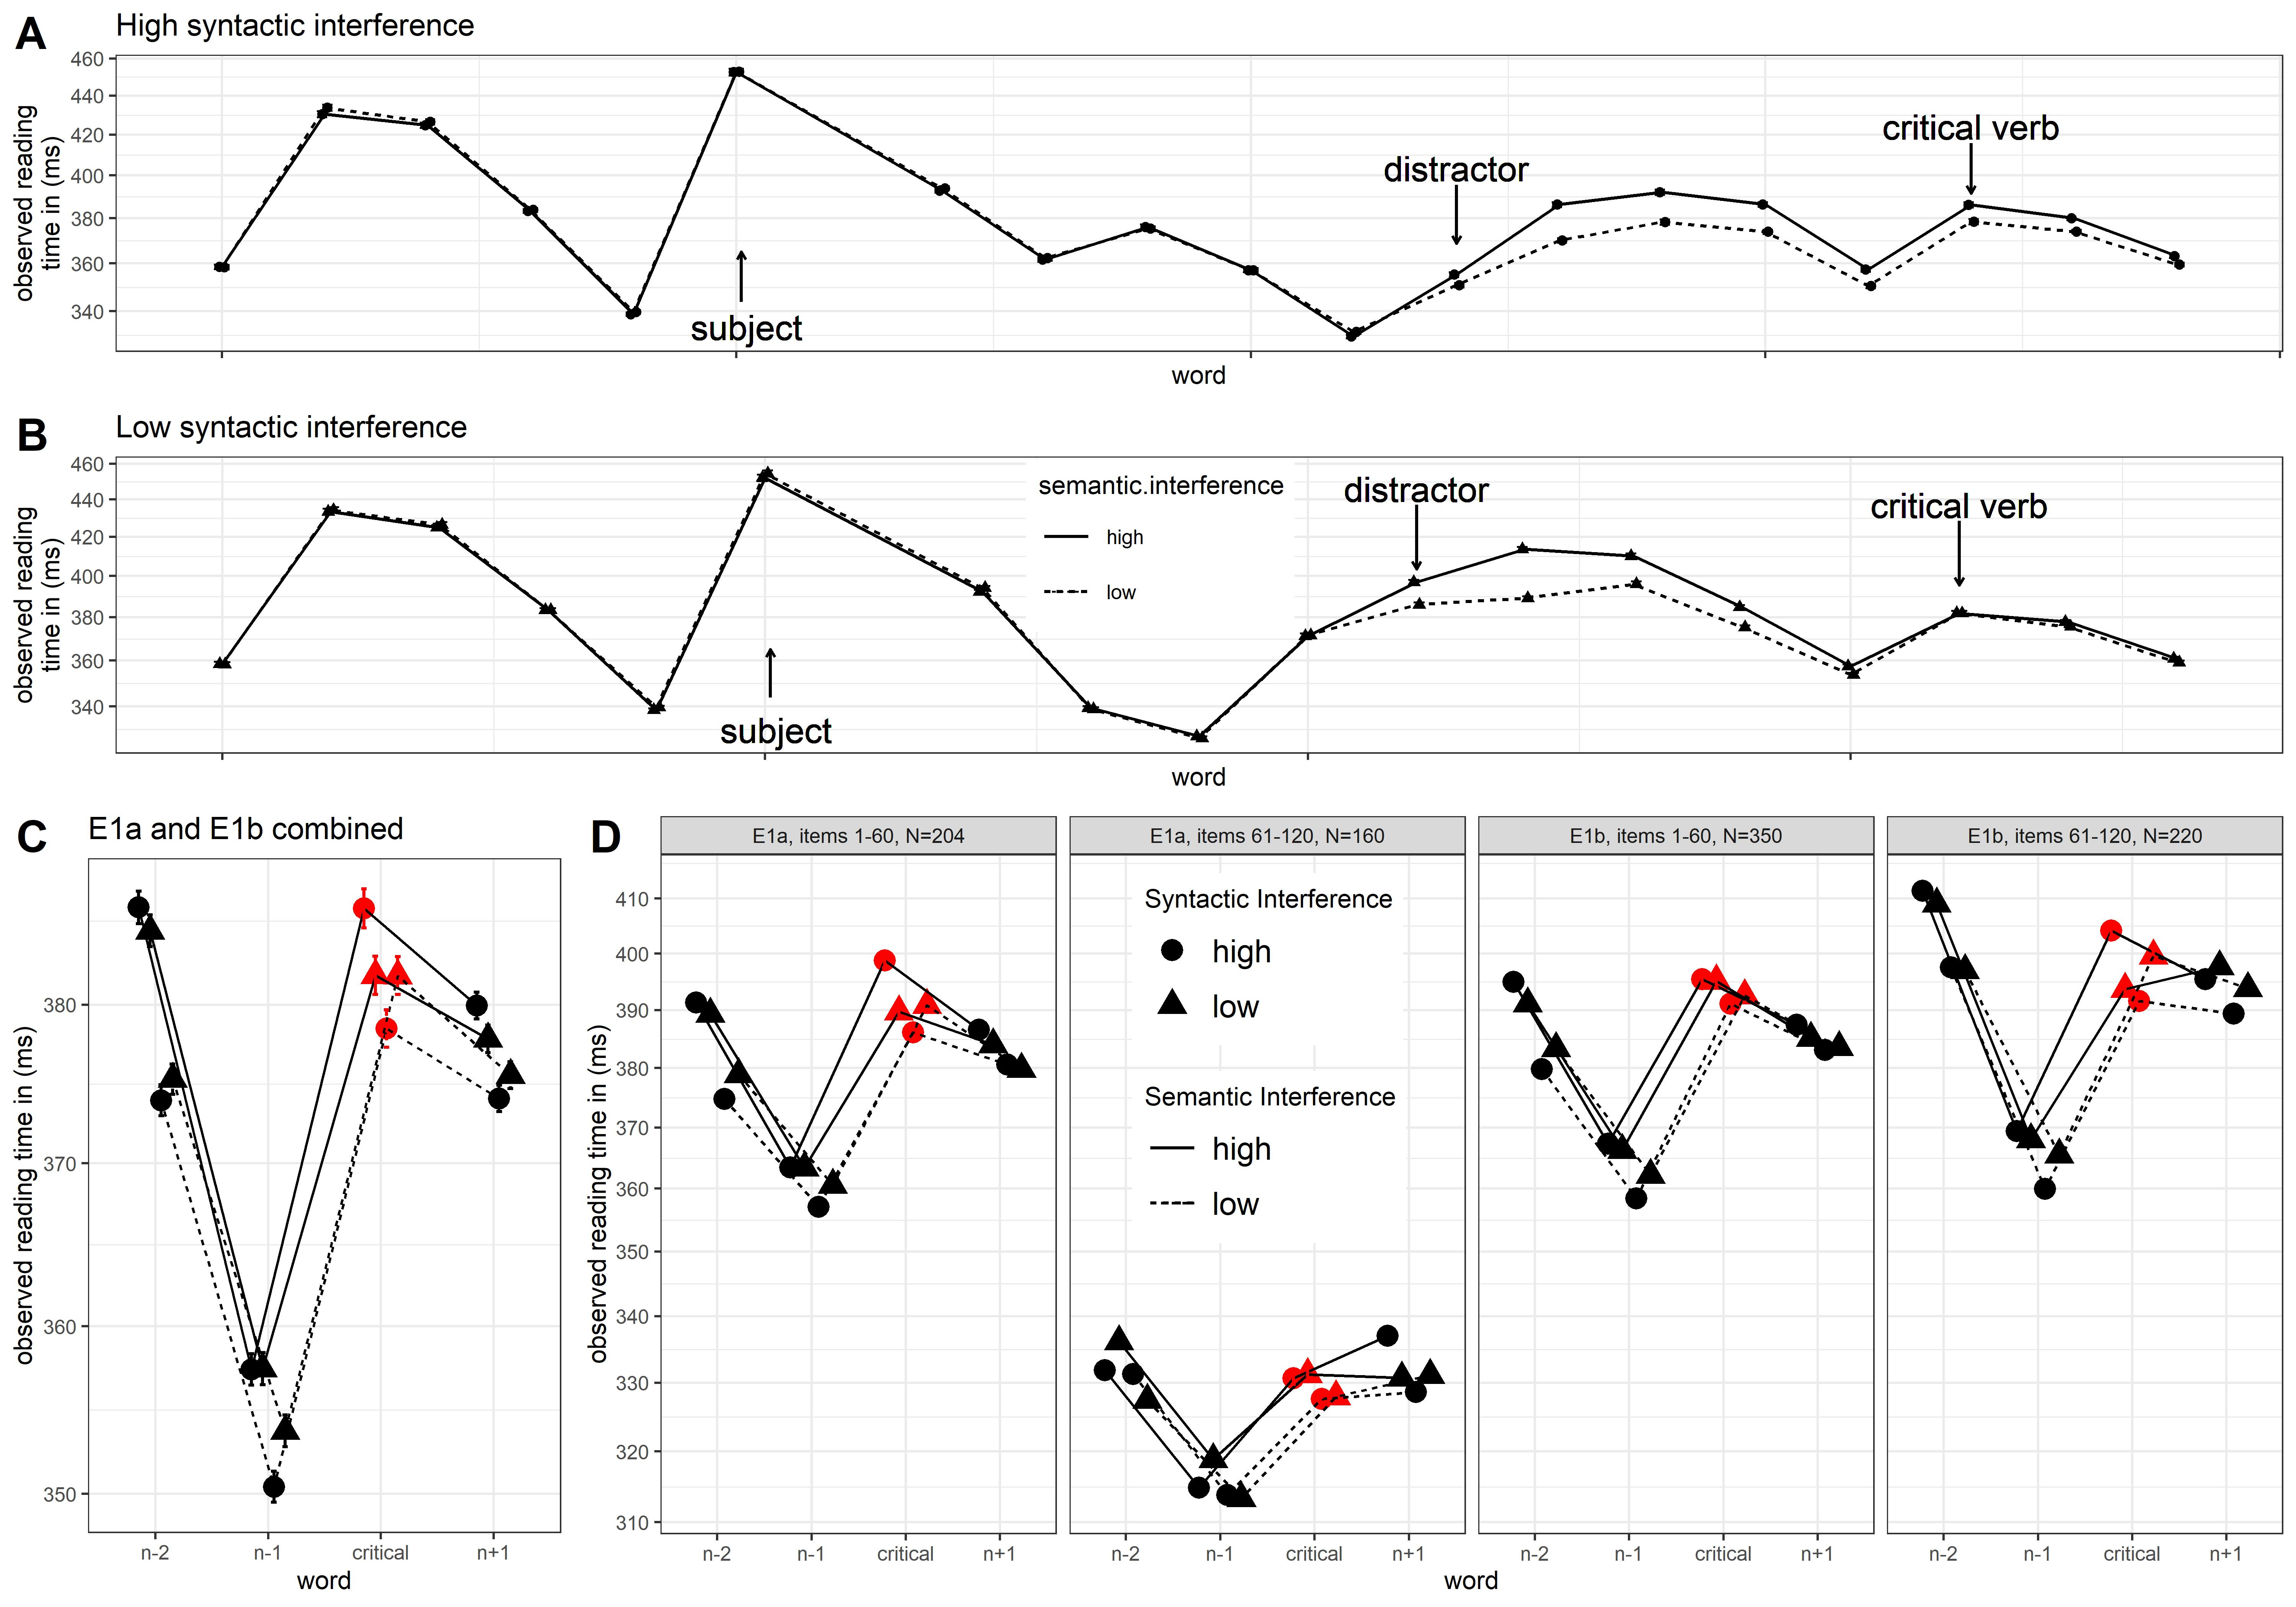
\includegraphics[width=0.85\textwidth]{images/Pandora_all_wholesentence_pooled_zoom_exp.jpg}
\end{sidewaysfigure}
\clearpage}

It is apparent from Figure \ref{fig:whole_sentence} A and B that, regardless of the syntactic manipulation, at the distractor, reading times between high and low semantic interference started to differ: distractors in the high semantic interference conditions induced longer reading times than in the low semantic interference conditions. This pattern persisted in the following regions.

Because the distractor and the immediately following regions differ between conditions, we did not compute Bayes factors for the observed reading time differences. Instead we focused our Bayes factors analyses on regions which were identical across conditions. These are the pre-critical, critical and spill-over regions.

Figure \ref{fig:whole_sentence} C shows the reading times of these regions; here, we also show the pre-pre-critical region, which was identical across conditions as well, but will be harder to interpret because of possible spill-over from the syntactic manipulation. The pre-pre-critical and pre-critical region show longer reading times for high vs.\ low semantic interference conditions. The critical verb was read slowest when syntactic and semantic interference were both high and fastest when syntactic interference was high and semantic interference low. The other two conditions showed intermediate reading times. The spill-over region again primarily showed a difference between high and low semantic interference conditions. 

Panels D and E show the reading times of the critical and surrounding regions for each of the two Experiments 1a and 1b. Panel D shows the results from Experiment 1a. The first session of Experiment 1a (items 1-60, N = 204, left sub-figure) showed results similar to the pooled results presented in Panel C. In the second session of Experiment 1a (items 61-120, N = 160, right sub-figure) a semantic interference effect was seen at the critical verb and the patterns in the surrounding regions were less clear than in the first session. Additionally, the second session in Experiment 1b showed shorter reading times compared to the first session. As mentioned earlier, this attenuation in reading times and differences between conditions are likely due to  adaptation to the SPR task in the second session. 

Panel E shows that Experiment 1b with items 1-60 (N = 350, left sub-figure) showed a pattern consistent with semantic interference in all regions. Experiment 1b with items 61-120 (N = 220, right sub-figure) showed a pattern consistent with semantic interference in the regions surrounding the critical verb, but not at the verb itself. At the verb, reading times were longest when both syntactic and semantic interference were high. Reading times were a bit faster when both syntactic and semantic interference were low. The other two conditions (high syntactic/low semantic and low syntactic/high semantic) lead to the fastest verb reading times in Experiment 1b with items 61-120. 

Turning now to the estimates of the main effects and interaction parameters in the pooled data (Experiments 1a and 1b combined), Figure \ref{fig:spr_posteriors} shows that the pre-critical, critical and spill-over regions showed very similar posterior distributions for the parameters. \Copy{SPR_results}{\textcolor{blue}{The 95\% credible intervals for syntactic interference were almost centered around zero in the pre-critical and critical regions. In the spill-over region, it included only positive values ([1, 15] ms). In contrast, for semantic interference, the 95\% credible intervals were fully positive in all regions; with identical estimates in the pre-critical and spill-over region ([7, 21] ms) and smaller estimates in the critical region ([1, 19] ms). The posteriors for the interaction were mostly positive, but the 95\% credible intervals included zero in all regions. The 95\% credible interval of the interaction was the widest in the critical region ([-3, 31 ms]) with a mean estimate of 14 ms.}

\begin{figure}[H]
    \caption{Posteriors for the syntactic and semantic interference effects and their interaction at the critical verb and surrounding regions in the pooled self-paced reading data (Experiments 1a and 1b combined). The numerical values are the means and 95\,\% credible intervals. The blue vertical lines represent the median and the blue shaded areas are 80\,\% credible intervals.}
    \label{fig:spr_posteriors}
    \centering
    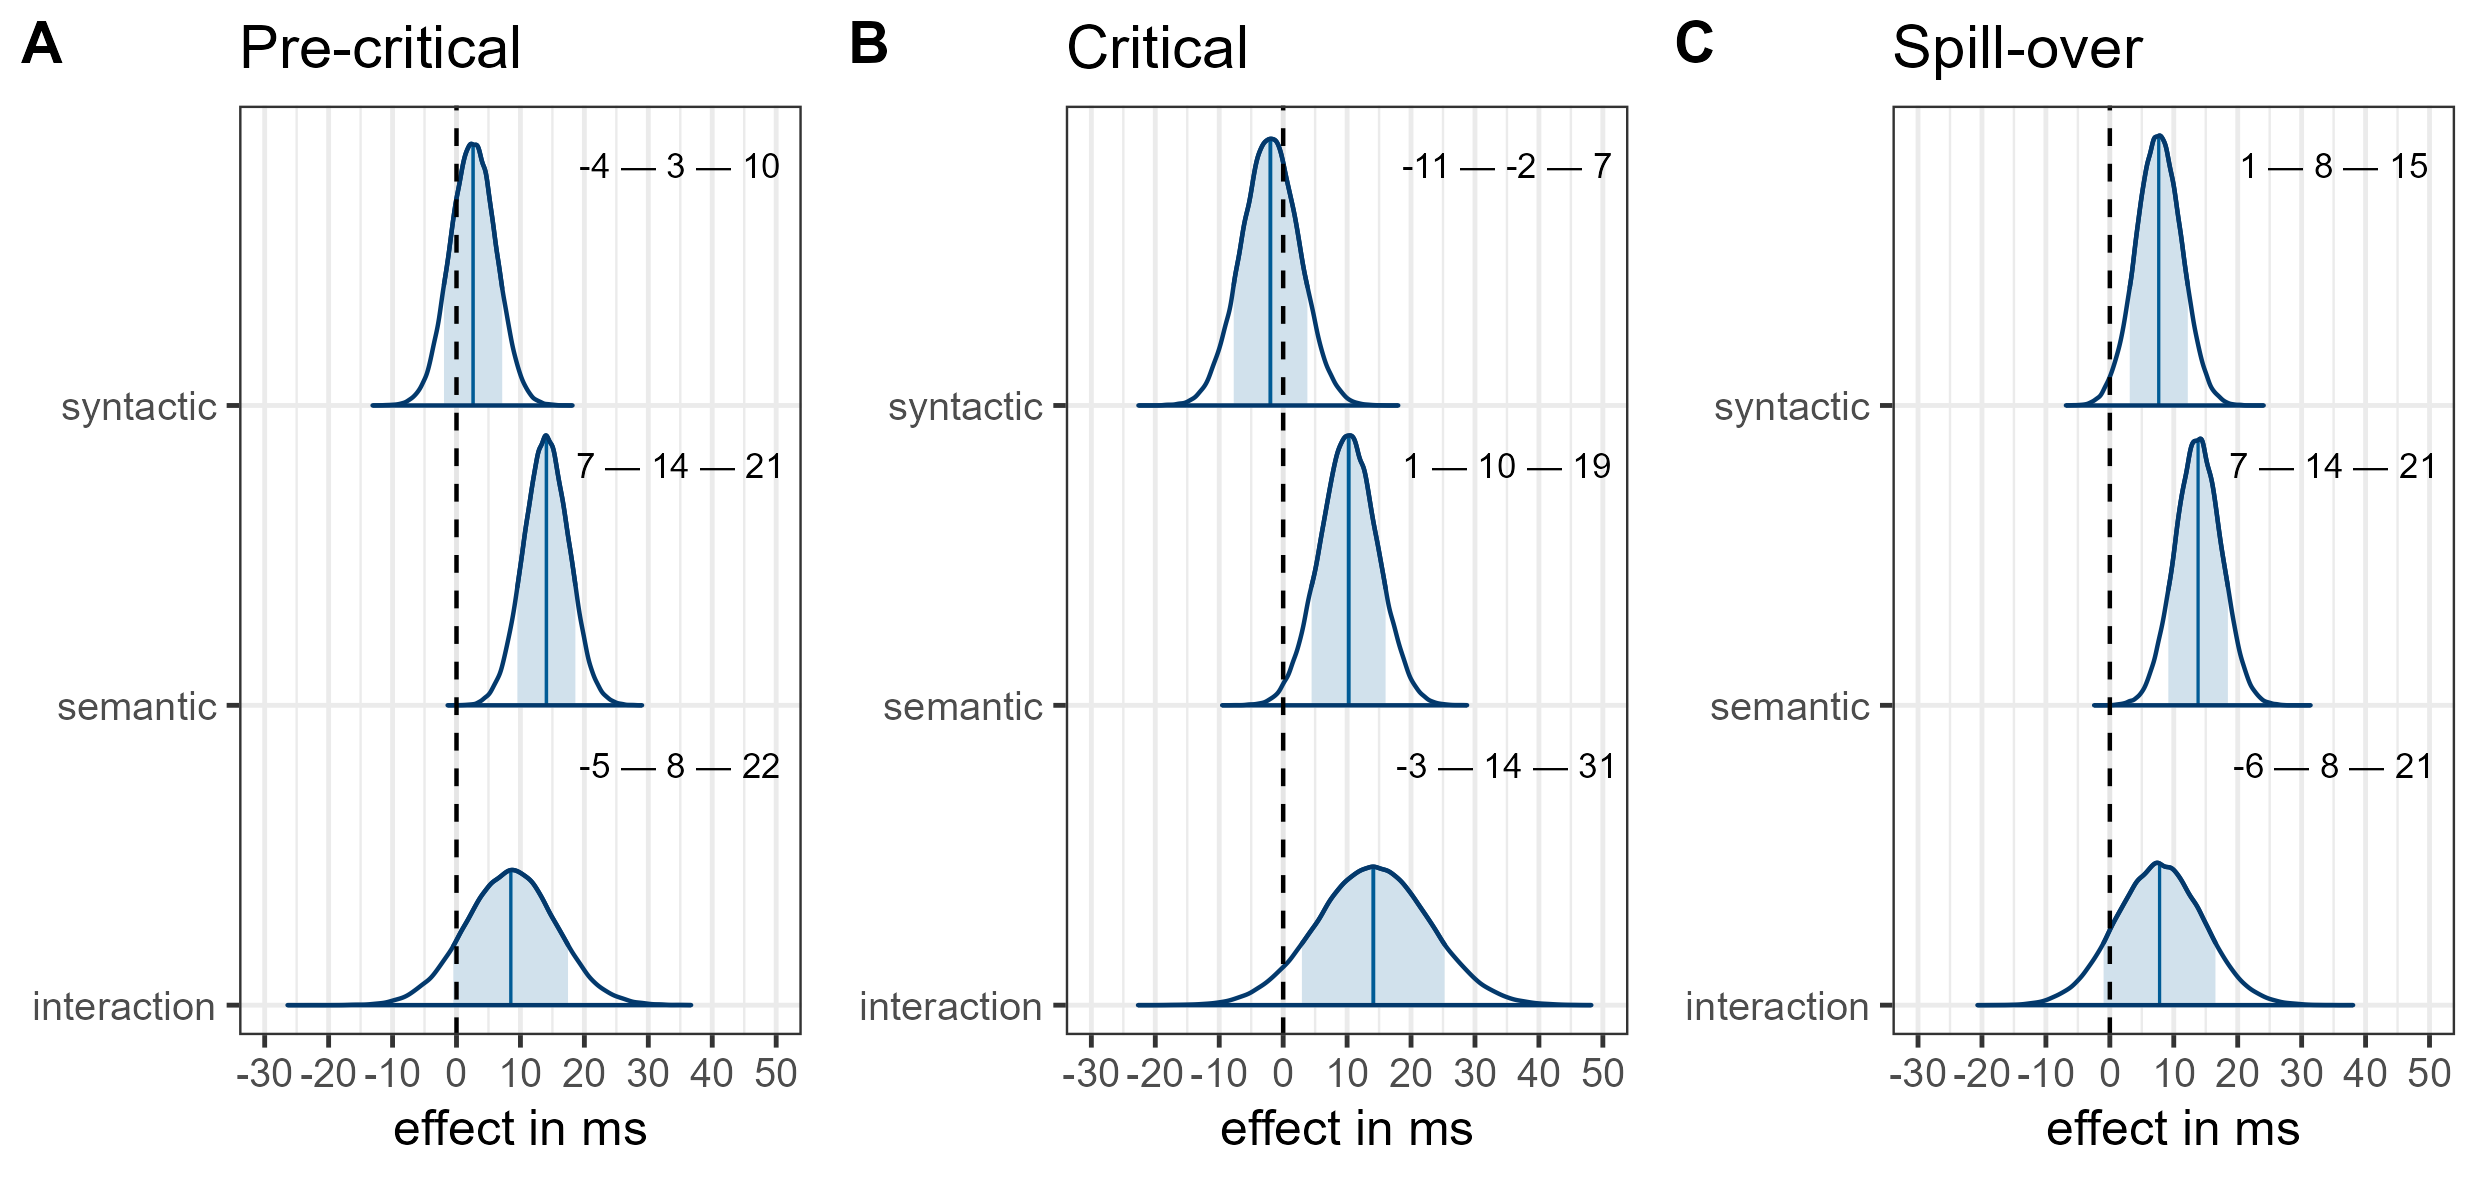
\includegraphics[width=\textwidth]{images/posteriors_spr_pooled_774.png}
\end{figure}
}\label{SPR_results}

\Copy{adaptation}{\textcolor{blue}{The fixed effect of trial id which was included in the models as a co-variate revealed a huge adaptation effect: From the first to the last trial (100th), reading times in the regions of interest decreased by on average around 250\,ms (pre-critical region: -219\,ms [-233, -204], critical region: -296\,ms [-317, -276], spill-over region: -246\,ms [-260, -233]). This adaptation effect was probably caused by increasing familiarity with the task and employed sentence structures over the time course of the experiment. While this adaption is interesting in itself, it is not the focus of the present study, therefore we will not discuss it further.}}\label{adaptation}

\paragraph{Hypothesis testing using Bayes factors}

Was there any evidence for the effects \textcolor{blue}{of interest }estimated above? The Bayes factor analysis is presented in Figure \ref{fig:spr_bfs}. The analyses use all the data from Experiments 1a and 1b. \Copy{SPR_bfs}{\textcolor{blue}{We found very strong to extreme evidence for the semantic interference effect in the pre-critical and spill-over region (BF$_{10}$ between 36 and 231). In the critical region, the evidence for semantic interference was inconclusive across the range of investigated priors (BF$_{10}$ between 0.7 and 3.5). There was evidence against an effect of syntactic interference under almost all priors in all regions (BF$_{10}$ $<$ 0.5). Only in the spill-over region when small effects between -8 and 8 ms were assumed a priori, there was anecdotal evidence for syntactic interference (BF$_{10}$ = 2.8). Similarly,} \Copy{insig_interaction}{\textcolor{blue}{there was overall evidence against the interaction of syntactic and semantic interference (BF$_{10}$ $<$ 1). Only under the narrowest prior in the critical region, there was very weak evidence for the interaction (BF$_{10}$ = 1.4).}}\label{insig_interaction}

\textcolor{blue}{All in all, the Bayes factor analysis provided very strong evidence for the semantic interference effect in the pre-critical and spill-over region, but inconclusive results in the critical region. In contrast, the Bayes factor analysis provided at best weak evidence for syntactic interference and the interaction or even evidence against them.}

\Copy{fig_bf_spr}{\begin{figure}[htpb]
    \caption{Bayes Factors for the effects of semantic interference, syntactic interference and their interaction in the reading times (combined Experiments 1a and 1b) at the critical verb and surrounding regions, under a range of priors on the target parameters.}
    \label{fig:spr_bfs}
    \centering
    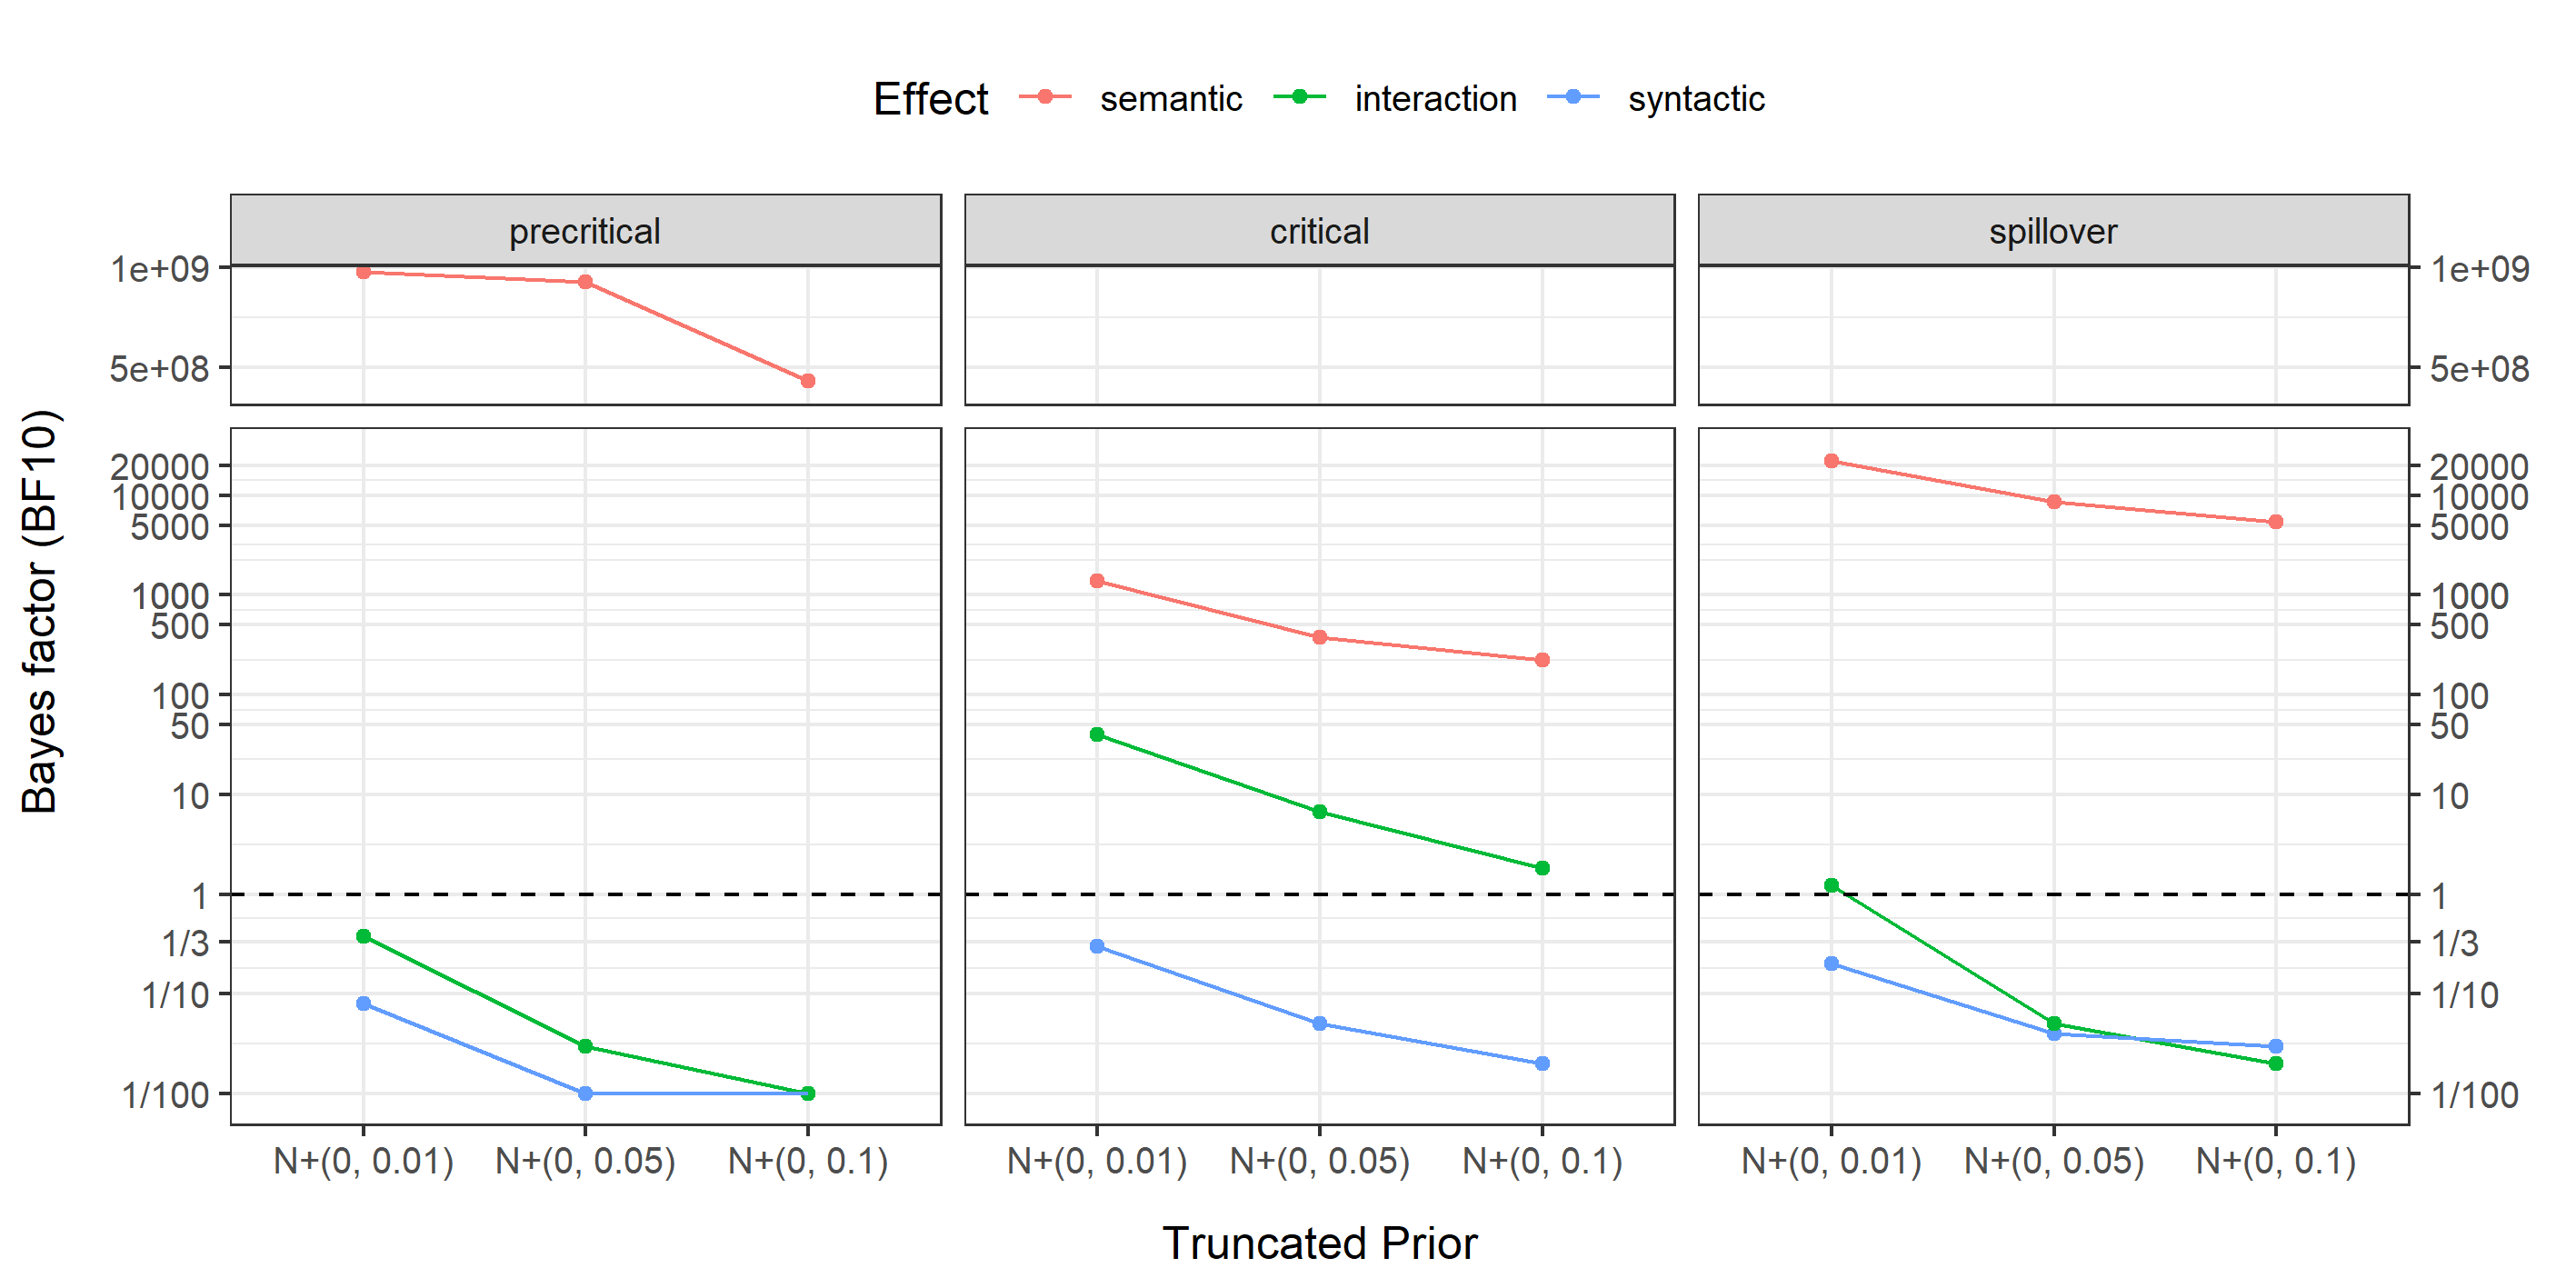
\includegraphics[width=\textwidth]{images/BF_plot_spr_774_allregions.png}
\end{figure}
}}

\subsection{Discussion}
We presented the to-date largest-sample self-paced reading study that investigated the use of syntactic and semantic features during subject-verb dependency formation. \textcolor{blue}{Reading times of the pre-critical word and critical verb showed evidence against syntactic interference. In the spill-over region, there was weak evidence for a small syntactic interference effect in the size of up to $\pm$8 ms. We will discuss the almost complete absence of syntactic interference in our data in the general discussion. The reading time results at the critical verb were inconclusive for semantic interference (BF$_{10}$ between 0.7 and 3.5 depending on a priori assumed effect size), but an effect of semantic interference was present at the regions surrounding the critical verb, i.e., the pre-critical and spill-over region. This means that semantic interference occurred even before the retrieval event could begin. Reading times at the critical verb showed very weak support for a small interaction of syntactic and semantic interference. There was evidence against the interaction under wider priors and in the surrounding regions.} \Copy{only_precritical}{\textcolor{blue}{Given the pre-critical reading times differences, effects in the later regions, i.e., the critical and spill-over region, cannot be attributed clearly to the stimuli in these regions and sentence processing mechanisms associated with them. Therefore, we refrain from discussing effects occurring in these regions.}}\label{only_precritical} The effects in the pre-critical region are discussed next.

\subsubsection{The effects in the pre-critical region}

At the distractor (which occurred well before the pre-critical region), high semantic interference (animate distractors) lead to longer reading times than low semantic interference (inanimate distractors, see Figure \ref{fig:whole_sentence} A and B). One might argue that this pattern could be due to differences in word length. The animate distractors in our materials were on average 1.1 letters longer than the inanimate distractors (mean length of animate distractors: 9.3, sd: 2.6, mean length of inanimate distractors: 8.2, sd: 2.9). It seems unlikely that this small difference of one letter in word length caused such large and long-lasting effects, but of course one cannot rule out this possibility with complete certainty.

\label{plausib_anim_inan}\Copy{plausib_anim_inan}{\textcolor{blue}{Another possible explanation for the reading time differences starting at the distractor could be a difference in plausibility between the high and low semantic interference conditions. To explore this possibility, we conducted a web-based plausibility judgement experiment on PCIbex  \parencite{pcibex}. Since we were only interested in the potential plausibility difference between the semantic interference conditions, we used a one-factorial design for the plausibility rating experiment investigating semantic interference within the high syntactic interference conditions (see \ref{ex:hisyn}, repeated here as \ref{ex:hisyn_repeat} for convenience). }

\begin{exe}  
\ex \label{ex:materials_repeat} Example item (critical word in bold, distractor in italics) of the present study:
    \begin{xlist}   
    \ex {High syntactic interference with high / low semantic interference:}\label{ex:hisyn_repeat} 
    \gll Die  Nachbarin glaubte,	dass	der Witwer,  der  erzählt hatte, dass der \textit{Einbrecher} / \textit{Verlust}  schrecklich war, abends regelmäßig \textbf{trank}, um zu vergessen.\\ 
    The\textsubscript{\sc{fem}} neighbor\textsubscript{\sc{fem}} believed that the widower who told had that the burglar / loss awful was in.the.evening regularly drank in.order to forget \\
    \trans `The neighbor believed that the widower, who had told her that the loss was awful, drank regularly in the evenings to forget.' \\
    \end{xlist}
\end{exe}

\textcolor{blue}{Forty-four native speakers of German (mean age: 26 years old, age range: 18 - 35 years, 21 female, 23 male), who were recruited over prolific and had not participated in the SPR experiment or norming study, provided ratings on a scale from 1 (absolutely implausible) to 7 (absolutely plausible). The mean ratings per item ranged from 3.6 to 6.6. The experiment included 40 implausible filler sentences which were created by exchanging nouns between the fillers used in the SPR experiment (e.g., Der Sohn des Kaisers, der den Feldzug gewonnen hatte, plante äußerst strategisch, weil er die Gießkanne an sich reißen wollte., `The son of the emperor who had won the campaign planned extremely strategically because he wanted to take the watering can by force.').  The mean rating of the implausible fillers ranged from 1.1 to 3.2. Participants spent approximately 37 minutes to complete the task and received \pounds 6.50 as compensation. The results of an ordinal brms model analyzing the ratings of the critical items are shown in Figure \ref{fig:plausibility_anim_inanim}. Sentences with an animate distractor had a slightly lower probability to gain a high rating on the plausibility scale ($\beta$ = -0.48, CrI [-0.67, -0.3]), i.e., the high semantic interference conditions were rated to be less plausible.}

\begin{figure}[htpb]
    \centering
        \caption{Posterior probability with 95\% credible intervals of each rating for items with inanimate and animate distractors.}
    \label{fig:plausibility_anim_inanim}
    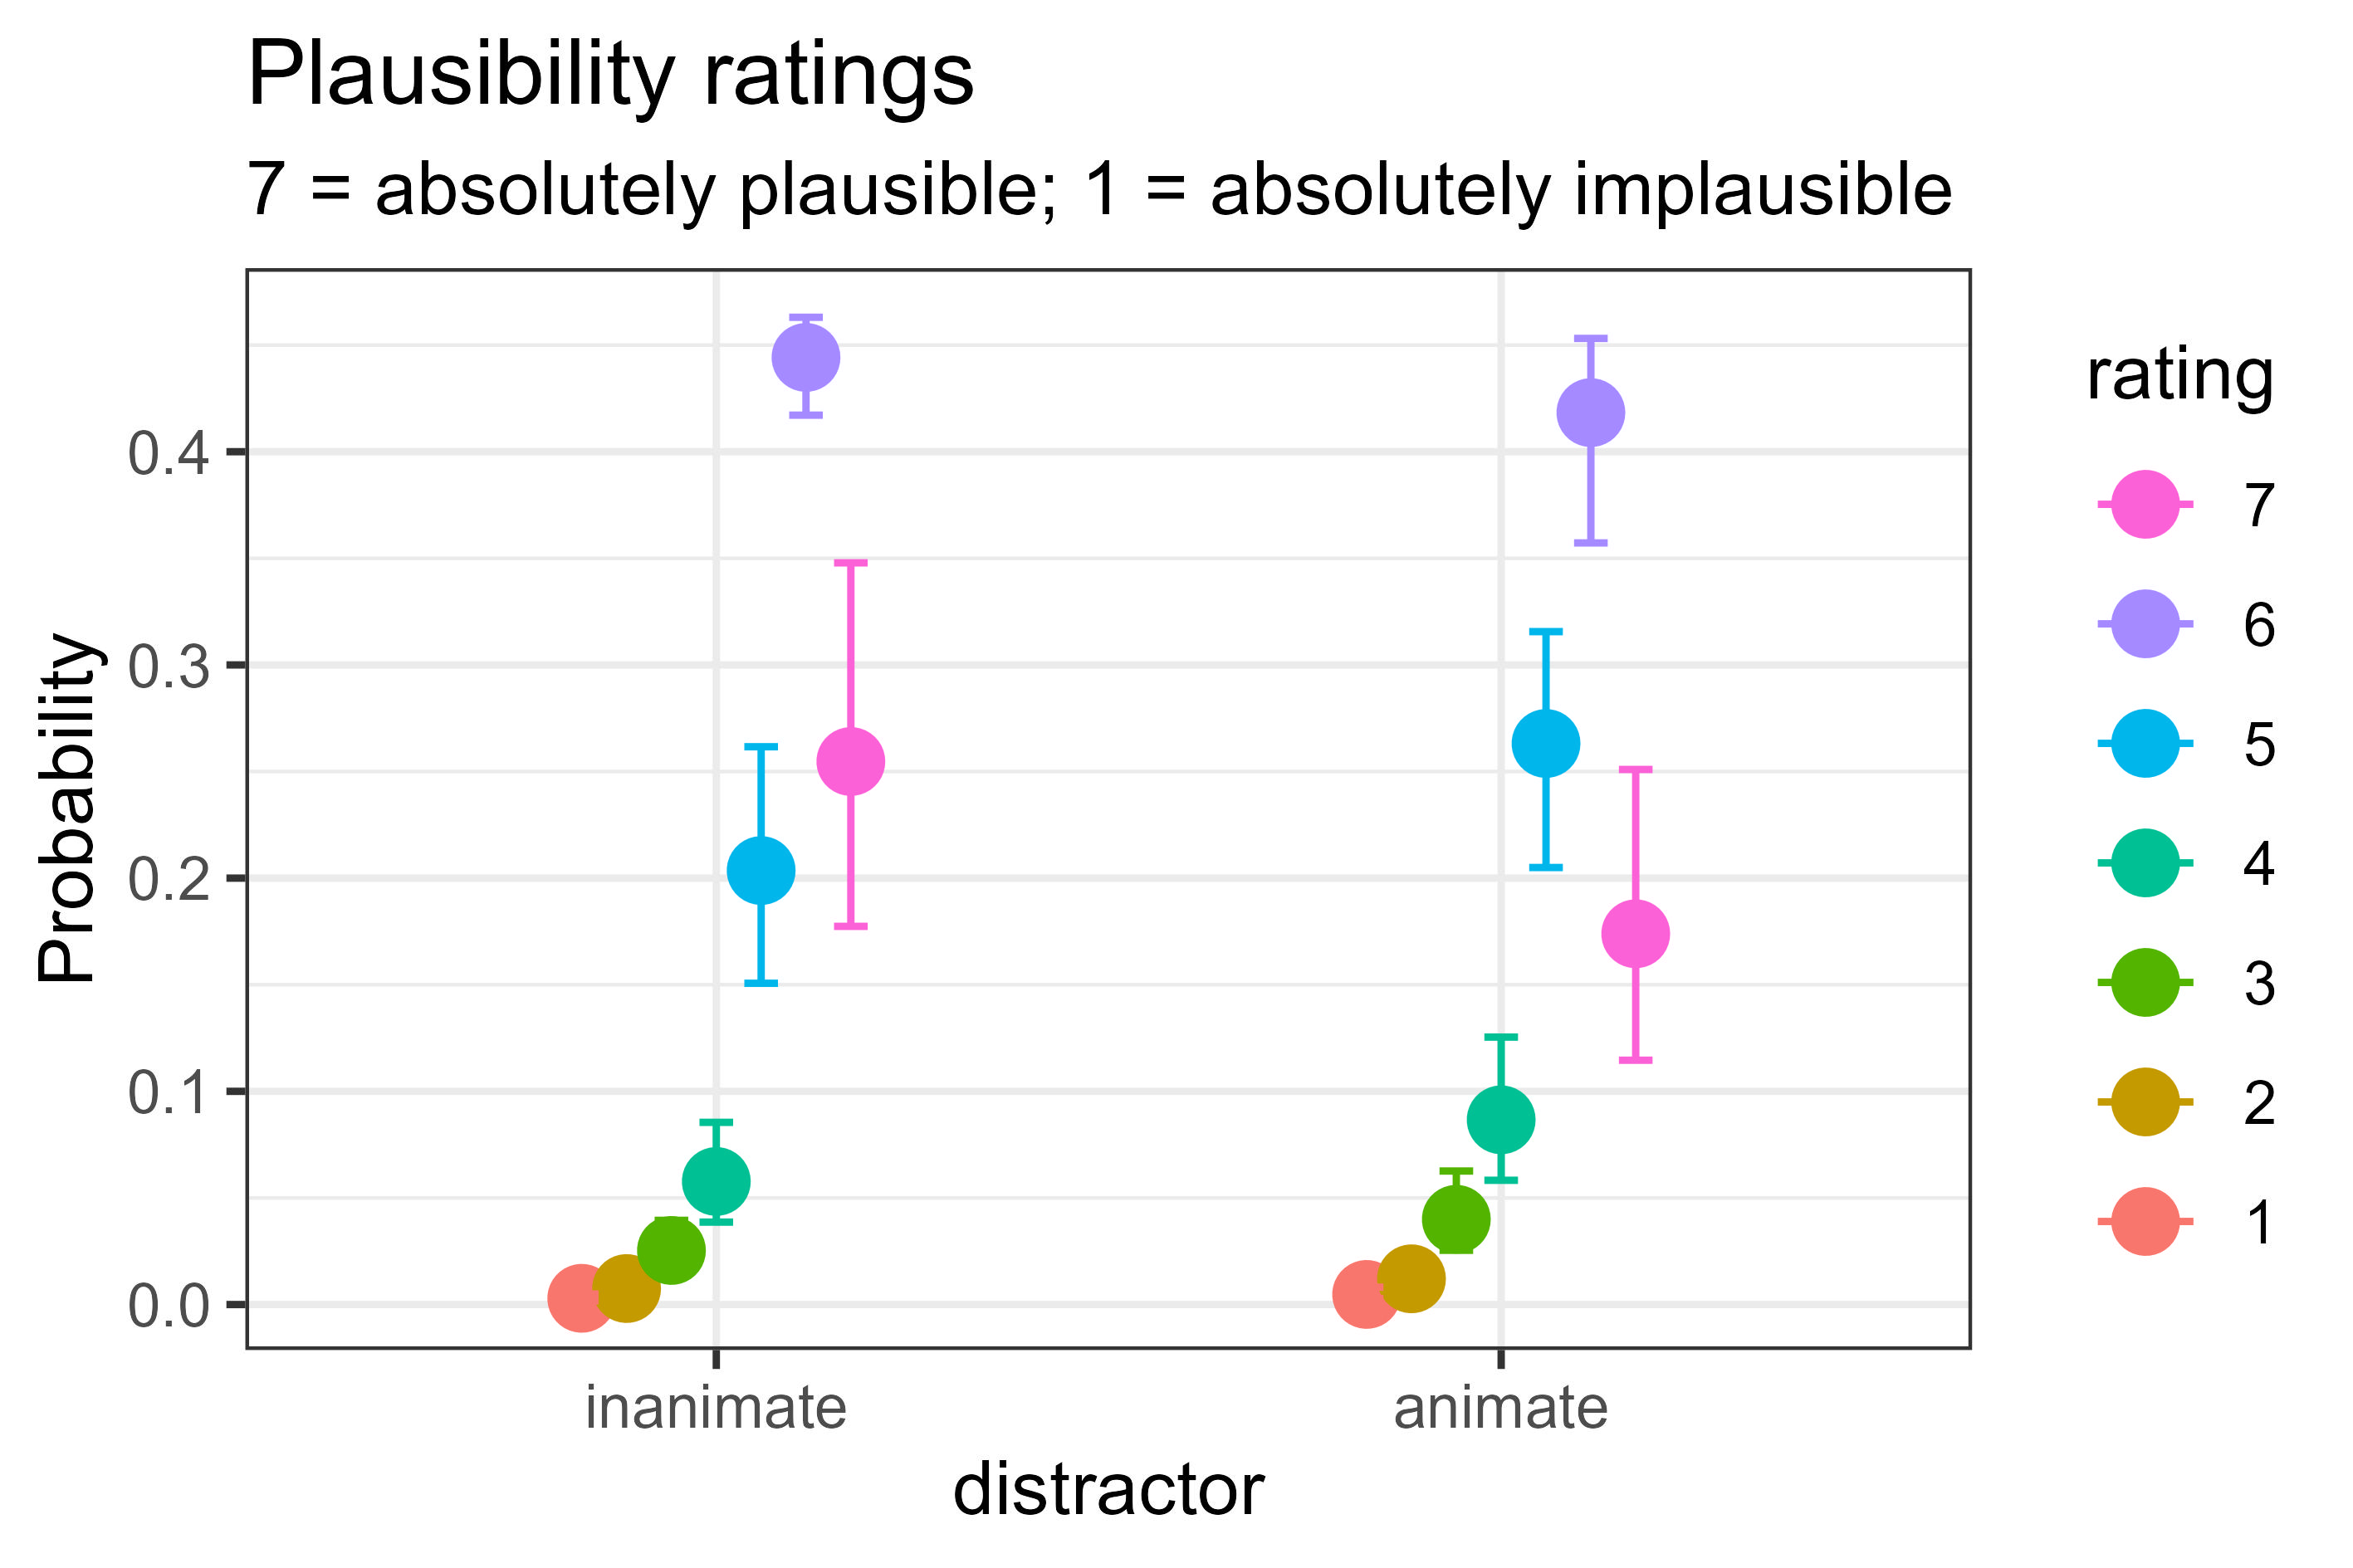
\includegraphics[width=0.8\linewidth]{images/plausibility_anim_inan.jpg}
\end{figure}

\textcolor{blue}{To investigate whether this plausibility difference is driving the semantic interference effect in our SPR data, we ran a Bayesian linear mixed model with log-normal likelihood on the reading times of the pre-critical region. This model included fixed effects for semantic interference (high +0.5, low -0.5), trial id (recoded to span from 0 to 1) and the centered plausibility ratings. We used the same priors as presented in Table \ref{tab:spr_priors}. The model was run with full random effects, i.e., varying intercepts and slopes of all fixed effects and their interactions by participants and items. Figure \ref{fig:posteriors_plausibility} presents the posteriors from the model with the Normal(0, 0.05) prior on the slopes. Although plausibility influenced reading times (higher plausibility lead to faster reading times, CrI [-30, -6] ms), there was an independent effect of semantic interference (CrI [2, 24] ms). The Bayes factors provided evidence for semantic interference in this analysis under all priors (Normal(0, 0.01): BF$_{10}$ = 4.2,
Normal(0, 0.05): BF$_{10}$ = 2.4,
Normal(0, 0.1): BF$_{10}$ = 1.3). The interaction of semantic interference and plausibility was centered around zero. In conclusion, the slowdown in the reading time results for high vs.\ low semantic interference was partially caused by reduced plausibility of the high semantic interference conditions. However, the plausibility difference was not the only driver of the reading time slowdown, i.e., semantic interference lead to slower reading times independent of plausibility.}

\begin{figure}
    \centering
        \caption{Posteriors of the semantic interference and plausibility effect and their interaction on the reading times in the pre-critical region. The numerical values are the means and 95\,\% credible intervals. The blue vertical lines represent the median and the blue shaded areas are 80\,\% credible intervals.}\label{fig:posteriors_plausibility}
    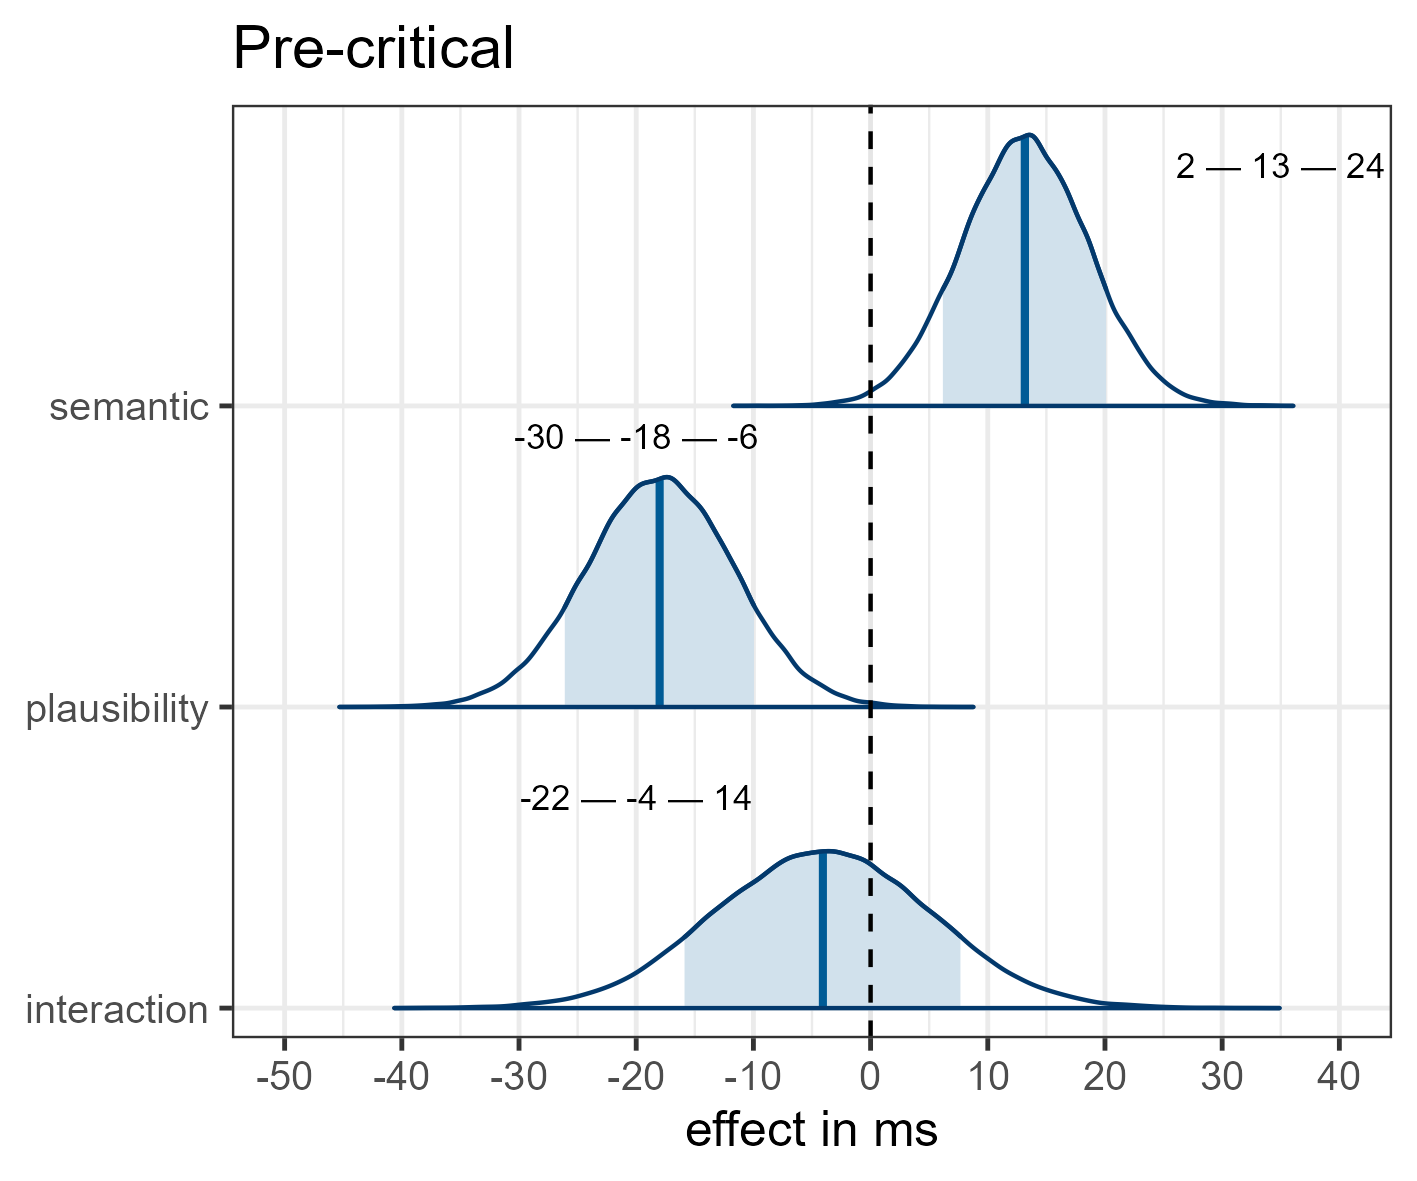
\includegraphics[width=0.8\linewidth]{images/posteriors_spr_pooled_774_plausibility.png}
\end{figure}
}

At the pre-critical region, there was evidence for semantic interference. As this cannot be due to retrieval interference, the most likely explanation is encoding interference (\cite{Oberauer_Kliegl_2006}\textcolor{blue}{, but see the potential confounds discussed above).} The increased effort of encoding and subsequently maintaining representations of three different animate noun phrases (the introduction noun, the subject and the animate distractor) is the most likely reason for the slowdown in high vs.\ low semantic interference conditions \citep[for similar findings, see e.g., ][]{lago_etal_2021, ness2019, ness2017, kush_etal_2015, gordon02}. 

Indeed, previous work using the same design as in the present paper has also found semantic interference effects at the pre-critical region: both \textcite{vandyke07} and \textcite{mertzen} found such effects. \citeauthor{mertzen}'s (\citeyear{mertzen}) Figures 5 and 6 indicated reading time differences in earlier regions, especially for their German data (see their Figure 6). \textcite{vandyke07} did not report reading times for the whole sentences / distractors;  \citeauthor{vandyke07} attributed the effects observed at the pre-critical region to plausibility differences between conditions, but as \textcite{mertzen} also points out, encoding interference could be an explanation even in that study. Given these earlier findings, our results are consistent with the encoding interference explanation.

\textcite{mertzen} observed both syntactic and semantic interference effects in the pre-critical region. 
They discuss several alternative explanations for their observed effects. In addition to encoding interference, \textcite{mertzen} propose three other alternative explanations for their data: parafoveal-on-foveal effects, sentence structure confounds across conditions, and predictive processing effects. Our results cannot be explained by the parafoveal-on-foveal explanation, because there is no parafoveal preview in self-paced reading. 

Regarding the possibility that sentence structure confounds as a possible explanation for the effects in the pre-critical region, this also seems implausible because the observed difference between the high and low semantic interference conditions is independent of the syntactic manipulation; it is the syntactic manipulation that has the confound. Therefore, the sentence structure confound is also not a good explanation for the semantic interference effect observed in our study. 

Regarding the predictive-processing explanation, \citet{mertzen} argued that the pre-critical adverb must attach to the upcoming verbal phrase; this leads to an anticipatory creation of a verb phrase chunk in memory, which triggers a retrieval of the subject already at the pre-critical region. However, in our study, the effect started at the distractor and became smaller as the two pre-critical adverbs were read (see Figure \ref{fig:whole_sentence} A and B). The predictive-processing explanation would incorrectly predict that the effect begins at the first adverb, which is the first word of the verbal phrase. Consequently, the prediction explanation is also ruled out in our data, rendering encoding interference the most likely explanation of the effects found prior to the critical verb in our data. Crucially, this line of reasoning should not be limited to the explanation of the pre-critical effects, but should be extended to the effects in the critical region as well. The reading times for high vs.\ low semantic interference conditions started to differ at the distractor and differed throughout the rest of the sentence. It is not possible to pinpoint whether the effect in the critical region is due to a retrieval initiated at this region, or still due to encoding and maintaining the distractor in memory \citep{ness2017}, or a combination of encoding and retrieval interference \parencite{Yadavetal2022}. Because of the unclear status of the effects at the critical verb, we refrain from interpreting the interaction which was only observed in this region. 

We turn next to the event-related potentials experiment.

\clearpage
\section{Experiment 2: EEG}
\subsection{Methods}
\subsubsection{Participants}
146 participants from the University of Potsdam participant pool took part in the experiment. Three participants were excluded because they did not fulfill the demographic requirements (bilinguals or medical history). Four participants were excluded because they finished only one out of two experimental sessions. Seven participants were excluded due to EEG artifacts (below 20 artifact-free trials in at least one condition). Additionally, 29 participants were excluded because they showed poor comprehension question accuracy (below 70\,\%) in one of the experimental sessions. The data of 103 participants (mean age: 23.5 years old, age range: 18 -- 38 years old, 81 female, 22 male) were used for the analyses presented here. These final participants were all right-handed, mono-lingual native speakers of German with normal or corrected-to-normal vision and no reported history of psychiatric or neurological disease. All participants gave written informed consent and were compensated with 40 Euros per experimental session (80 Euros in total) or course credit.

\subsubsection{Procedure}
The experiment was conducted in two experimental sessions for practical reasons (each of the sessions lasted approximately two hours). Sessions were separated by one to eight weeks for each participant (the median gap was two weeks, the first and third quartiles being one and three weeks). \Copy{fillers2}{The procedure of both sessions was identical \textcolor{blue}{and the same lists were used as in Experiment 1, with 60 critical sentences and 40 fillers per session}.

During each experimental session, the EEG was recorded while participants were seated in a sound-proof booth. OpenSesame was used to present sentences word-by-word \citep{opensesame}. Participants were familiarized with the procedure with two practice sentences. After that, the experiment was conducted in four blocks of \textcolor{blue}{25} sentences each, presenting the items in pseudorandomized order, with breaks between the blocks.}\label{fillers2} Each trial started with the presentation of a fixation cross in the center of the screen for 500 ms. Next, each word of the sentence was presented in the center of the screen. Word duration for words of interest (subject, distractor, pre-pre-critical word, pre-critical word, critical verb, post-critical word) was 500 ms. Word duration of all other words was 190 ms + 20 ms per character of the specific word. The inter-stimulus interval between all words was 400 ms. After a third of the trials, participants were asked to answer yes/no comprehension questions by pressing one of two keys on a standard keyboard. The j key was always mapped to ``yes'' answers and the f key was always mapped to ``no'' answers. The correct response was counterbalanced, so that half of the time a ``no'' response was correct and half of the time a ``yes'' response was correct.

\subsubsection{EEG recording and processing}
The EEG was recorded with 24 Ag/AgCl scalp electrodes, positioned according to the international 10-20 system. During recording, an electrode at the left mastoid was used as reference and AFz as ground. The sampling rate was 500 Hz. Eye-movements were monitored with six electrodes which were positioned above, below and at the outer canthus of both eyes. Impedances of all electrodes were kept below 5\,k$\Omega$.

Processing of the EEG data was carried out with MNE python \citep{mne}. The EEG was offline re-referenced to the average of the left and right mastoid electrodes. Eye-movements were corrected using independent component analysis (ICA) based on bipolar electro-oculogram channels. The data was band-pass filtered between 0.1 and 30 Hz. The data was segmented into epochs starting 200 ms preceding critical verb onset and lasting until 1000 ms following critical word onset. Epochs with artifacts were excluded automatically.

\subsubsection{Statistical analyses}
The statistical analyses of the comprehension accuracy in the EEG experiment were carried out in the same manner as the analyses of the comprehension accuracy in the SPR experiment.

We used Bayesian linear mixed models to analyze the single trial EEG data in response to the critical verb. We averaged the activity of 12 centro-parietal electrodes (Cz, C3/4, CPz, CP1/2, CP5/6, Pz, P3/4, POz) in the standard \textcolor{blue}{time windows of the  N400 (300 to 500 ms post critical word onset) and P600 (600 to 900 ms post critical word onset)} for all analyses. The models included sum-contrast coded fixed effects for syntactic interference (high +0.5, low -0.5), semantic interference (high +0.5, low -0.5) and their interaction. In addition to the fixed effects of interest, all models included the baseline EEG activity from 200 ms prior to critical word onset until critical word onset as a continuous predictor. This functioned as a regression-based instead of traditional baseline correction \citep{alday2019}. Varying intercepts for participants and items as well as by-participant \textcolor{blue}{and by-item} random slopes for \textcolor{blue}{syntactic interference,} semantic interference \textcolor{blue}{and their interaction} were included. We used relatively informative priors for all parameters of the models (see Table \ref{tab:eeg_priors}). 

\begin{table}[!htbp]
    \caption{Relatively informative priors for the analysis of the event-related potentials \citep{nicenboim_stats}. The standard deviations of the slope priors were varied in order to conduct a Bayes factor sensitivity analysis. See the corresponding assumed a priori range of the difference between high vs.\ low interference.}
    \label{tab:eeg_priors}
    \centering
    \begin{tabular}{llr}
    \toprule
    Parameter&Prior &Assumed Range ($\mu V$)\\
    \midrule
  Intercept & \textcolor{blue}{Normal(0, 5)}& \textcolor{blue}{[-10, 10]}\\
  \cmidrule{2-3}
  \multirow{4}{1cm}{slope} & \textcolor{blue}{Normal(0, 0.1)} & \textcolor{blue}{[-0.2, 0.2}]\\
  & \textcolor{blue}{Normal(0, 0.5)}& \textcolor{blue}{[-1, 1]}\\
  & \textcolor{blue}{Normal(0, 1)} & \textcolor{blue}{[-2, 2]}\\
  & \textcolor{blue}{Normal(0, 2)} & \textcolor{blue}{[-4, 4]}\\
  \cmidrule{2-3}
  sigma & Normal(10, 5)&\\
  SD & Normal(0, 2)&\\
    \bottomrule
    \end{tabular}
\end{table}

Bayesian models were run with four chains and 20,000 iterations of which 2,000 were used as warm-up phase \citep{schad_etal_2022_BF}. For the calculation of Bayes factors and the corresponding sensitivity analysis, we defined a range of priors on the parameters of interest, assuming a range of effect sizes \citep{nicenboim_stats,schad_etal_2022_BF}. We chose slope priors which assume a wide range of effect sizes from \textcolor{blue}{[$-0.2$, 0.2] to [$-4$, 4]\,$\mu V$}. 

\subsection{Results}
\subsubsection{Comprehension question accuracy}
After exclusion of participants with accuracy below 70\,\%, the overall accuracy (including fillers) was 82.8\,\% (range: [71.9, 100]\,\%). Accuracy in critical trials was 75.6\,\% ([55, 95]\,\%). By-condition accuracy is presented in Table \ref{tab:eeg_acc}. 

\begin{table}[]
    \caption{By-condition accuracy in critical trials in the EEG experiment.}
    \label{tab:eeg_acc}
    \centering
    \begin{tabular}{llr}
    \toprule
    syntactic & semantic & accuracy \%\\
    \midrule
        low &  low & 81.6\\
        low &  high & 74.0\\
        high &  low & 85.1\\
        high &  high & 68.1\\
    \bottomrule
    \end{tabular}
\end{table}

Table \ref{tab:eeg_acc_mod} presents the results of the generalized mixed model analyzing the comprehension accuracy in the critical trials. The log-odds estimates and 95\,\% credible intervals show reduced comprehension accuracy in high compared to low semantic interference conditions. Additionally, the results suggest an interaction, i.e., the difference between high and low semantic interference conditions was larger when syntactic interference was high vs.\ when it was low. Because the accuracies are not of primary interest, we did not carry out Bayes factors analyses for these.

\begin{table}[]
    \caption{Results in log-odds from a Bayesian generalized model analyzing the comprehension accuracy in critical trials of the EEG experiment.}
    \label{tab:eeg_acc_mod}
    \centering
    \begin{tabular}{lrr}
    \toprule
    & Estimate &  95\% CrI  \\
    \midrule
Intercept& 1.39 &   [1.10, 1.68]\\
syntactic& -0.04 &  [-0.16, 0.08]\\
semantic&  -0.48 & [-0.61, -0.36]\\
interaction& -0.17&  [-0.34, -0.01]\\
    \bottomrule
    \end{tabular}
\end{table}

\subsubsection{Event-related potentials}

\paragraph{Estimated effect sizes and their uncertainty}

Figure \ref{fig:erp_all} shows the 
grand average ERPs elicited by the critical verb for all conditions. \textcolor{blue}{Figure \ref{fig:eeg_posteriors} shows the estimates for the brain activity in the spatio-temporal windows of the N400 and P600 from the linear mixed models with prior Normal(0, 0.5) which assumed interference effects with a difference possibly as large as $\pm$1\,$\mu V$. }\Copy{ERP_results1}{\textcolor{blue}{The 95\% credible intervals of the semantic interference effect showed more negative brain responses for high vs.\ low interference and did not include zero for both the N400 and the P600. The 95\% credible intervals of the syntactic interference effect also showed more negative brain responses for high vs.\ low interference, but the mean estimate was about half the size of the semantic interference estimate, respectively, and the intervals included zero for both the N400 and the P600. The 95\% credible interval of the interaction was centered around zero for the N400. For the P600, it included mostly negative values but crossed zero.}}\label{ERP_results1}

\begin{figure}[H]
    \caption{ERPs elicited by the critical verb (word onset at 0\,ms) at electrode Cz.}
    \label{fig:erp_all}
    \centering
    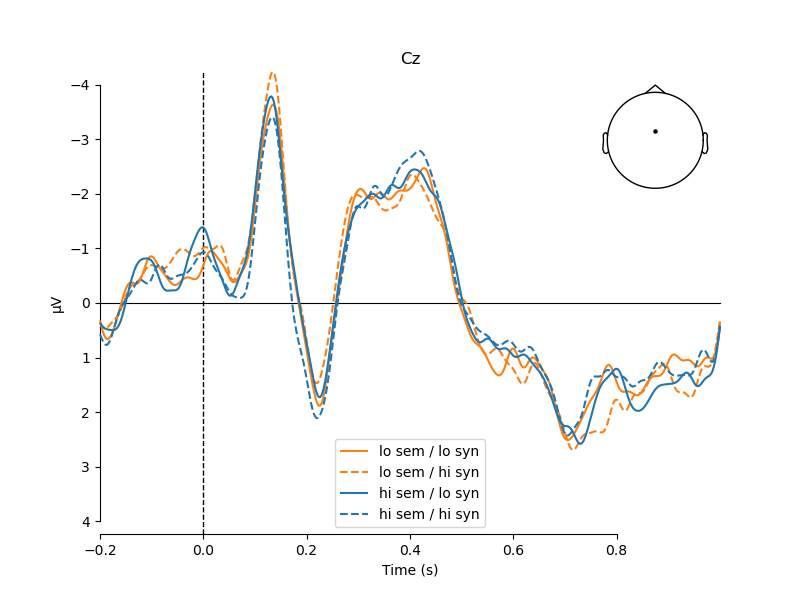
\includegraphics[width=\textwidth]{images/N_103_Cz_crit.png}
\end{figure}

\begin{figure}[H]
    \caption{Posteriors of the syntactic and semantic interference effects and their interaction for the event-related potentials elicited by the critical verb in the spatio-temporal \textcolor{blue}{windows of the N400 (A) and P600 (B)}. Blue vertical lines represent the median and shaded areas are 80\,\% intervals.}
    \label{fig:eeg_posteriors}
    \centering
    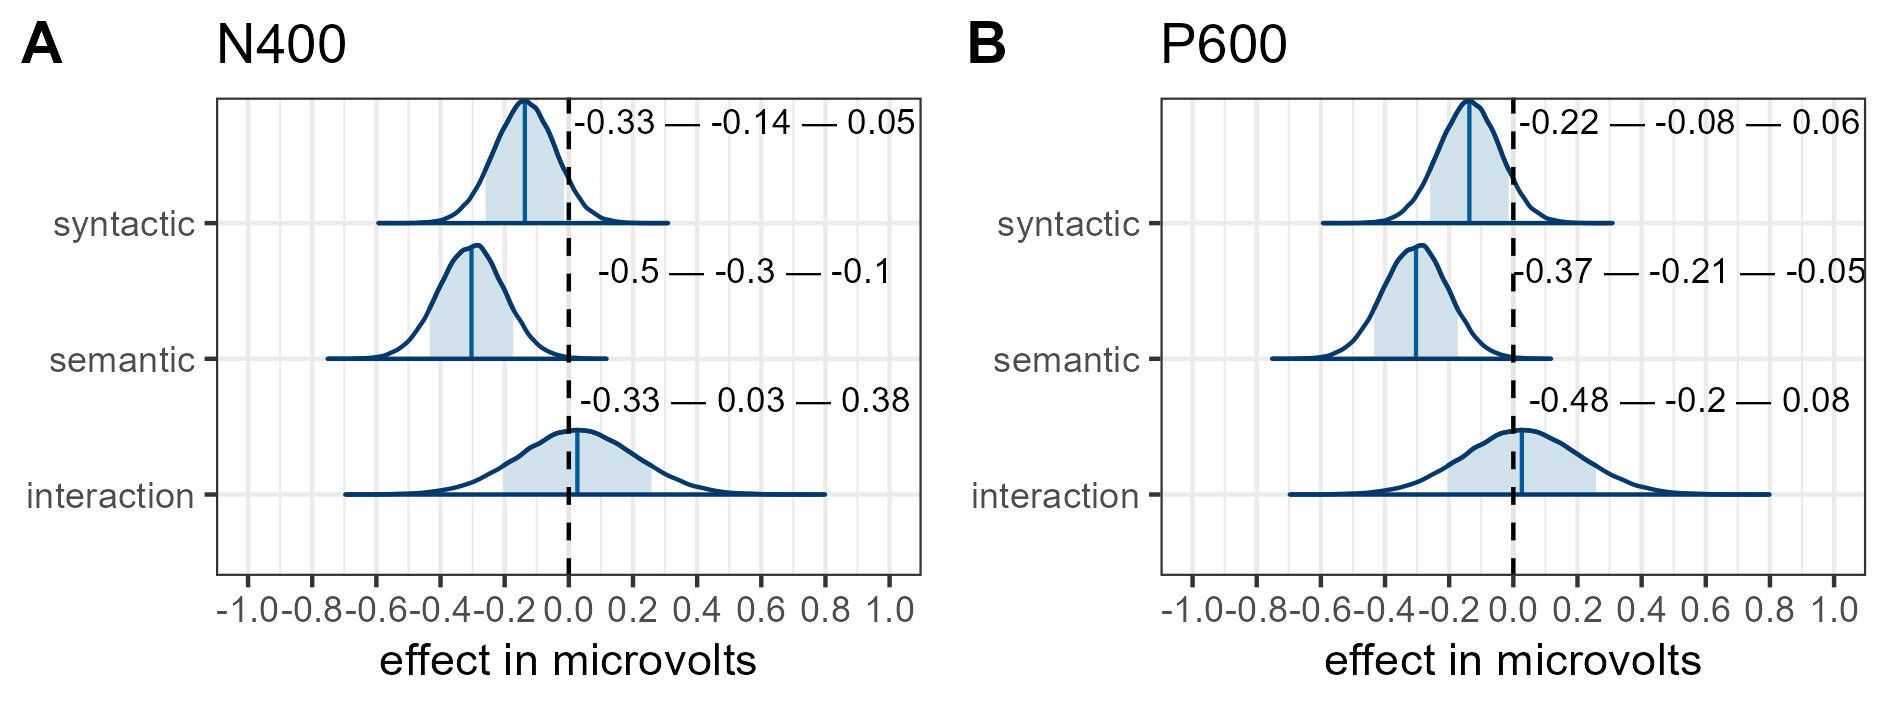
\includegraphics[width=\textwidth]{images/posteriors_eeg.jpg}
\end{figure}


The semantic interference effect is further illustrated in Figure \ref{fig:erp_sem_syn} (a) and (b). Figure \ref{fig:erp_sem_syn} (a) shows that around 400 ms, the critical verb elicited a more negative ERP under high than under low semantic interference. Figure \ref{fig:erp_sem_syn} (b) shows that the topography of the effect is rather broad but with a concentration of more negative values at centro-parietal electrodes. The timing and topography of this effect suggested that it was an N400 effect; thus, the N400 was modulated by semantic interference. \textcolor{blue}{Furthermore, Figure \ref{fig:erp_sem_syn} (a) shows a slightly reduced P600 amplitude for high vs.\ low semantic interference. See Figure \ref{fig:erp_sem_syn} (c) for the topographic distribution of this effect.} \Copy{ERP_results2}{In contrast, Figure \ref{fig:erp_sem_syn} (d), (e) and (f) show that syntactic interference did not considerably affect the brain response to the critical verb in \textcolor{blue}{neither the N400 nor P600 spatio-temporal windows}.}\label{ERP_results2} Visual inspection of the ERPs in \ref{fig:erp_sem_syn} (d) does also not suggest that there was a syntactic interference effect in any other time window.

\begin{figure}[H]
\caption{Brain responses elicited by the critical verb. (a) ERPs for semantic interference (word onset at 0\,ms) at electrode Cz. Topographic maps of the semantic interference effect (high semantic interference - low semantic interference) in the N400 time window (b) and P600 time window (c). (d) ERPs for syntactic interference  (word onset at 0\,ms) at electrode Cz. Topographic maps of the syntactic interference effect (high syntactic interference - low syntactic interference) in the N400 time window (e) and P600 time window (f).}
    \label{fig:erp_sem_syn}
\begin{minipage}{.74\linewidth}
\centering
\subfloat[]{\label{fig:erp_sem_ERP}
\includegraphics[scale=.62]{images/ERP_animacy_Cz.png}}
\end{minipage}%
\begin{minipage}{.25\linewidth}
\centering
\subfloat[]{\label{fig:erp_sem_topo}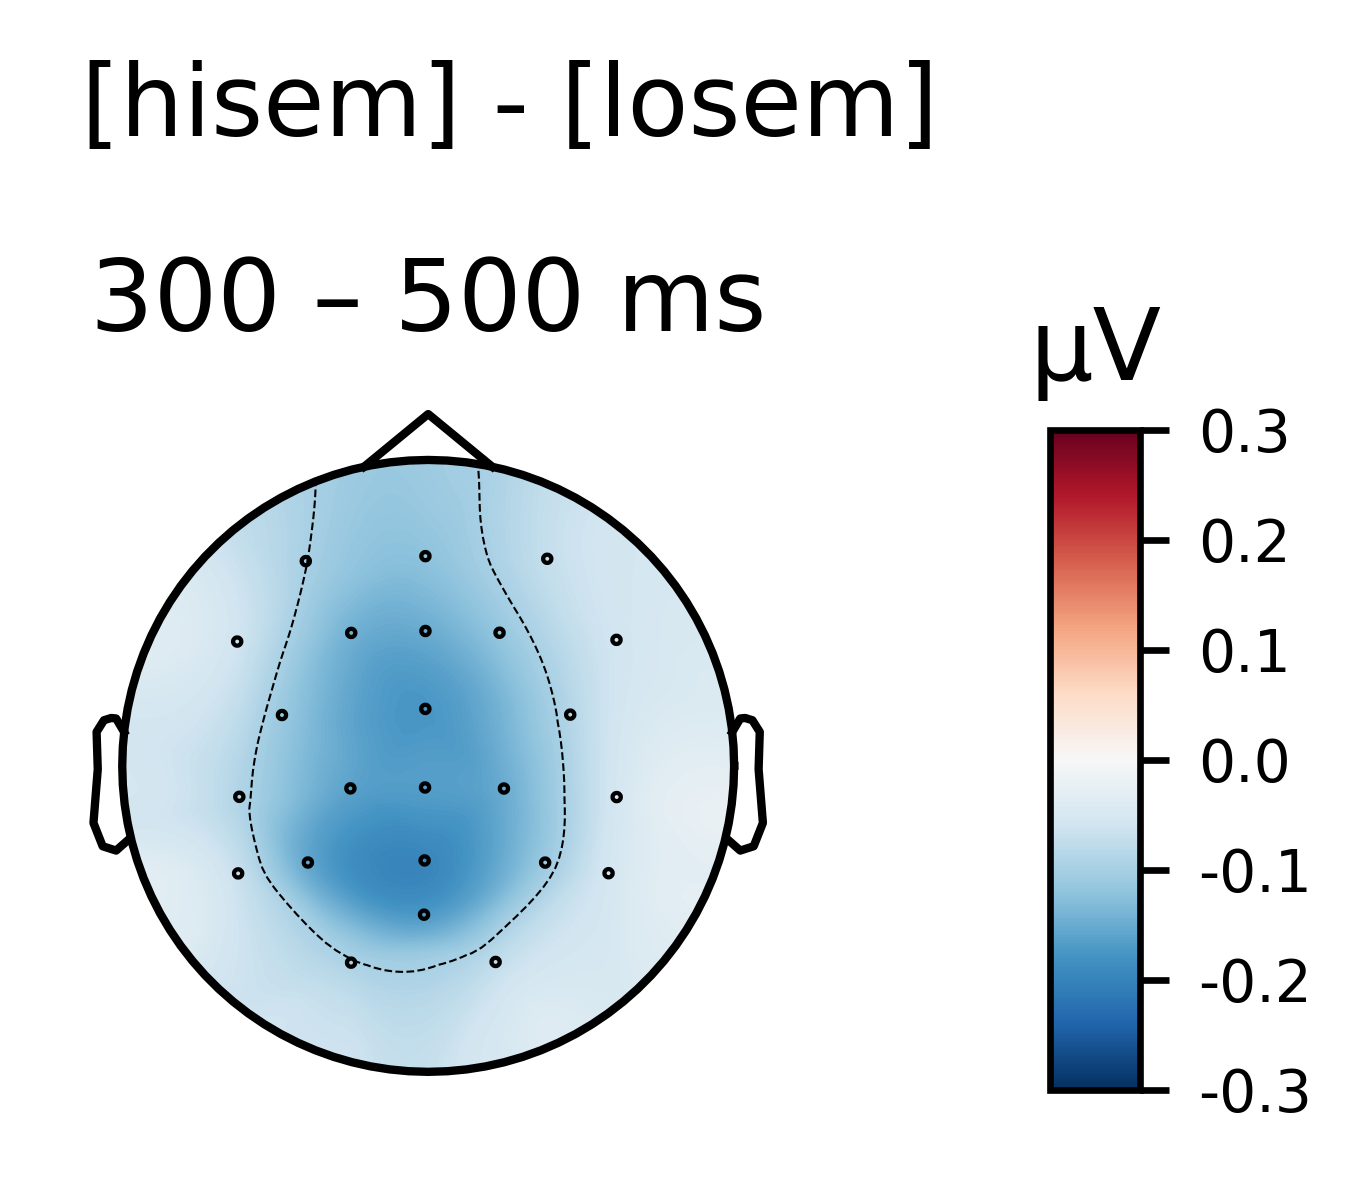
\includegraphics[scale=.65]{images/topo_animate-inanimate_300_500.png}}
\par\medskip
\centering
\subfloat[]{\label{fig:erp_sem_topo_p600}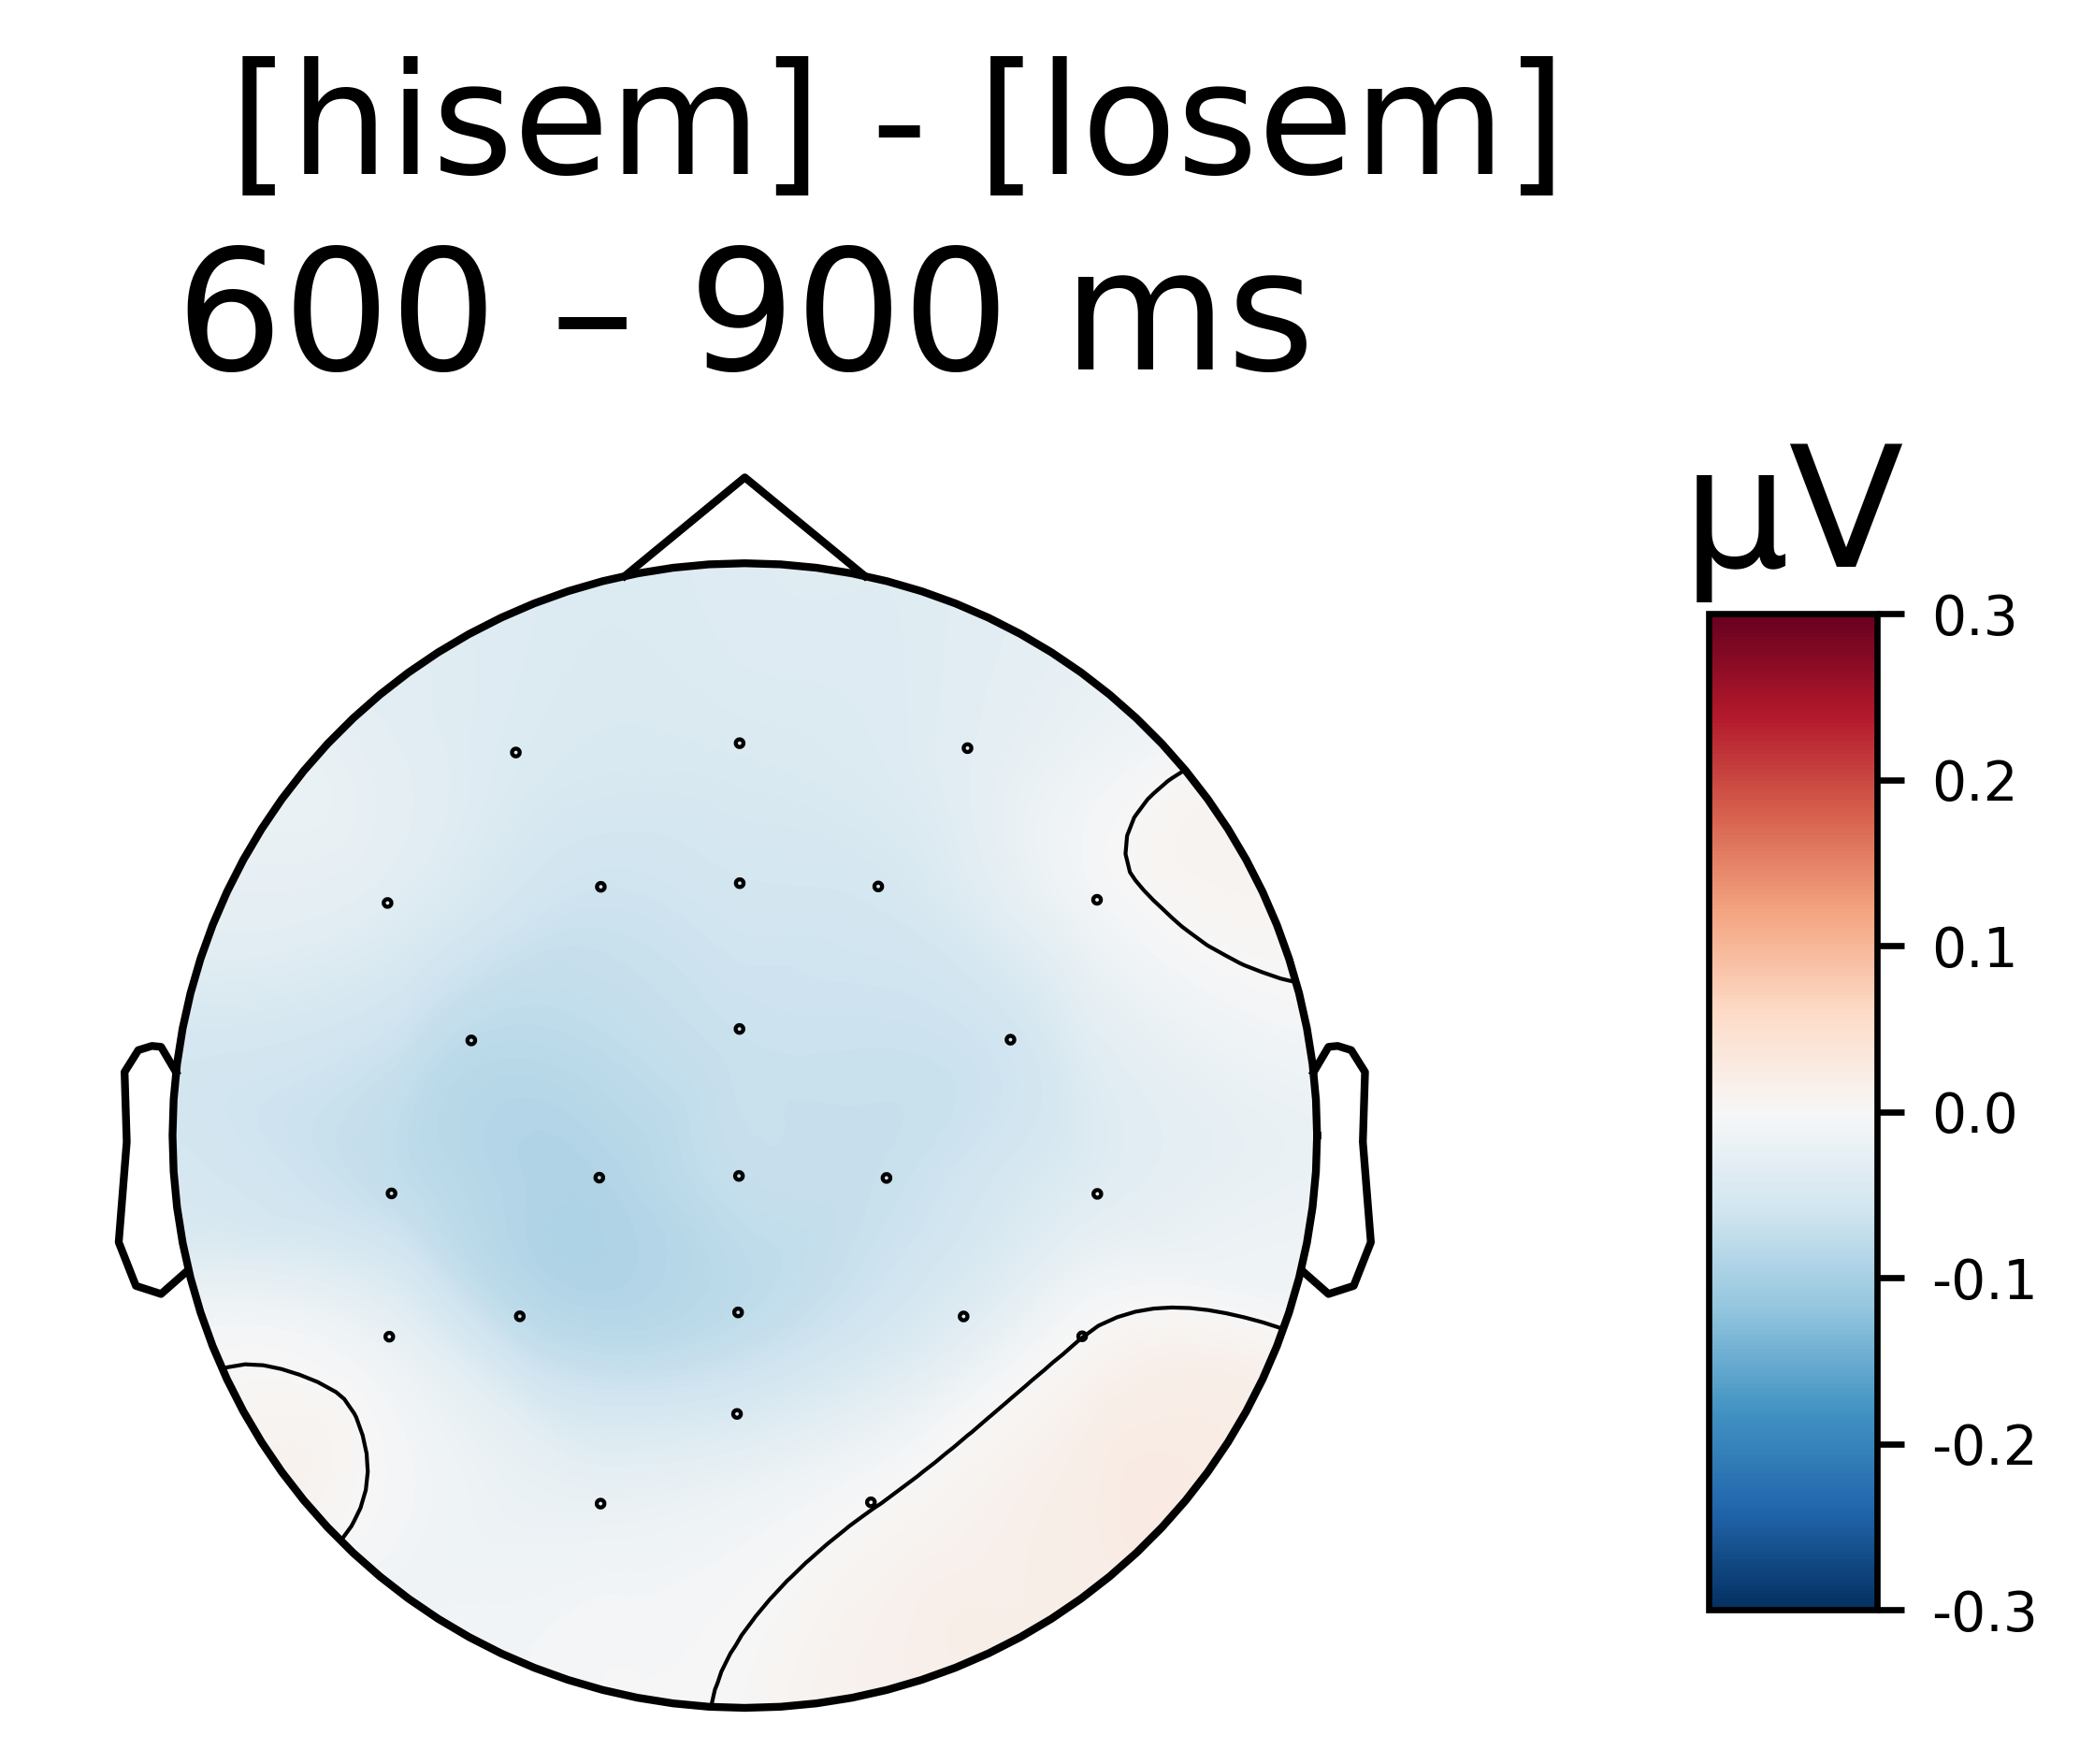
\includegraphics[scale=.65]{images/topo_animate-inanimate_600_900.png}}
\end{minipage}
\begin{minipage}{.74\linewidth}
\centering
\subfloat[]{\label{fig:erp_syn_ERP}
\includegraphics[scale=.62]{images/ERP_subj_Cz.png}}
\end{minipage}%
\begin{minipage}{.25\linewidth}
\centering
\subfloat[]{\label{fig:erp_syn_topo}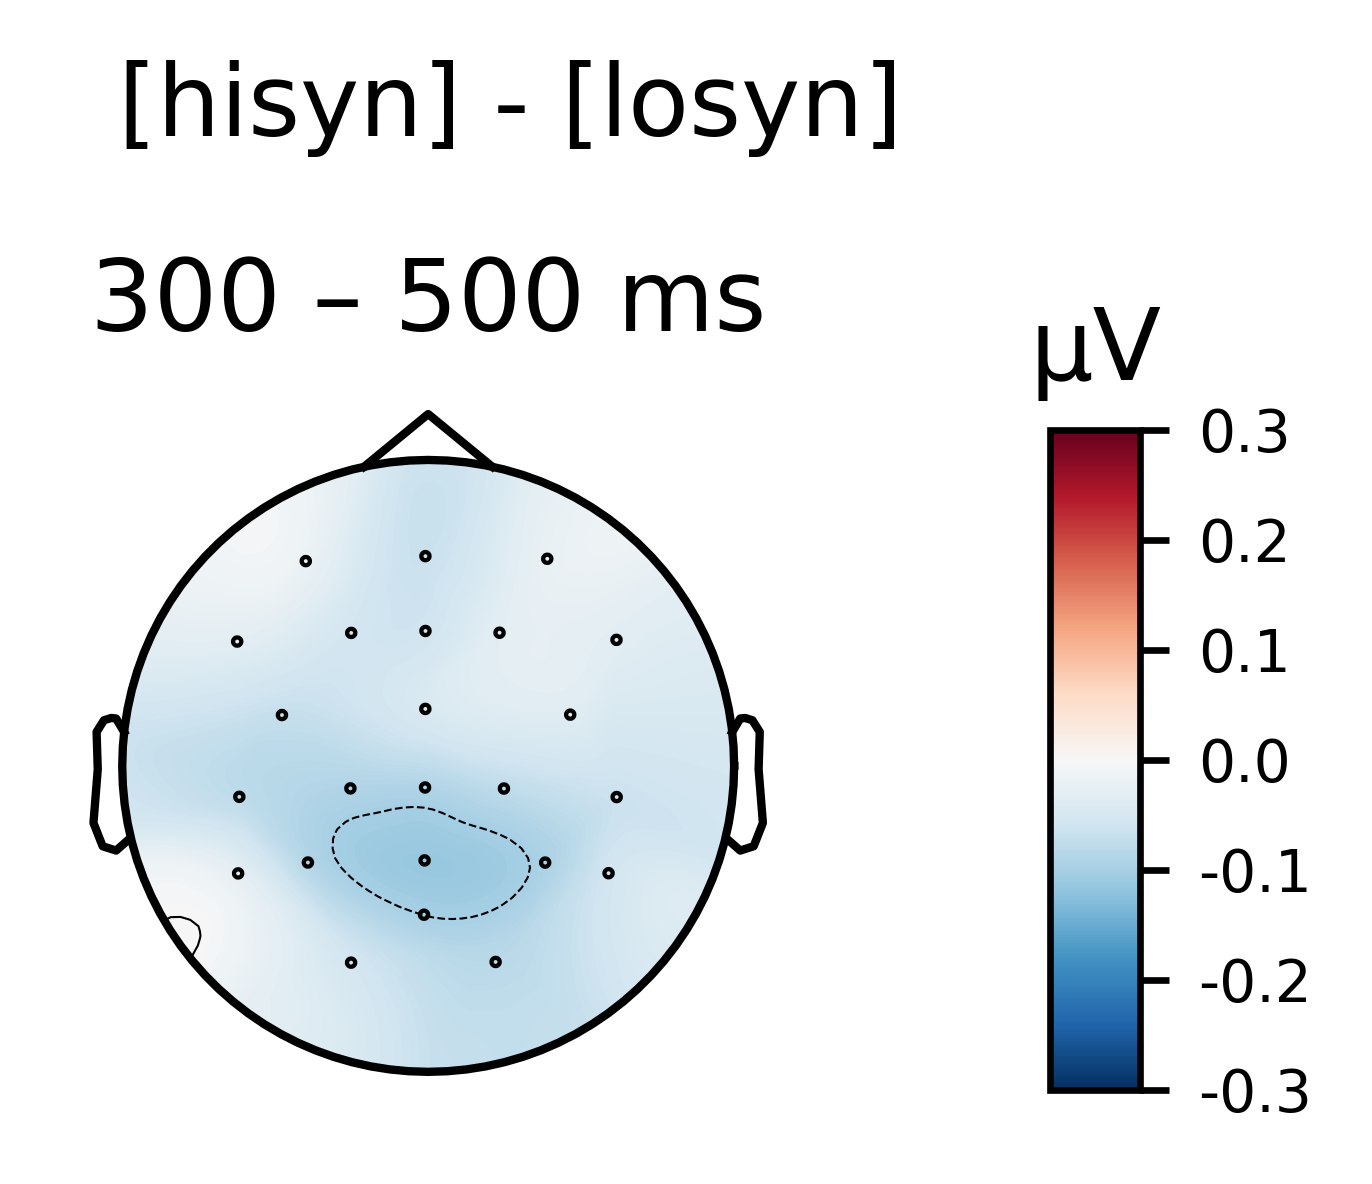
\includegraphics[scale=.65]{images/topo_subj-nsubj_300_500.png}}
\par\medskip
\centering
\subfloat[]{\label{fig:erp_syn_topo_p600}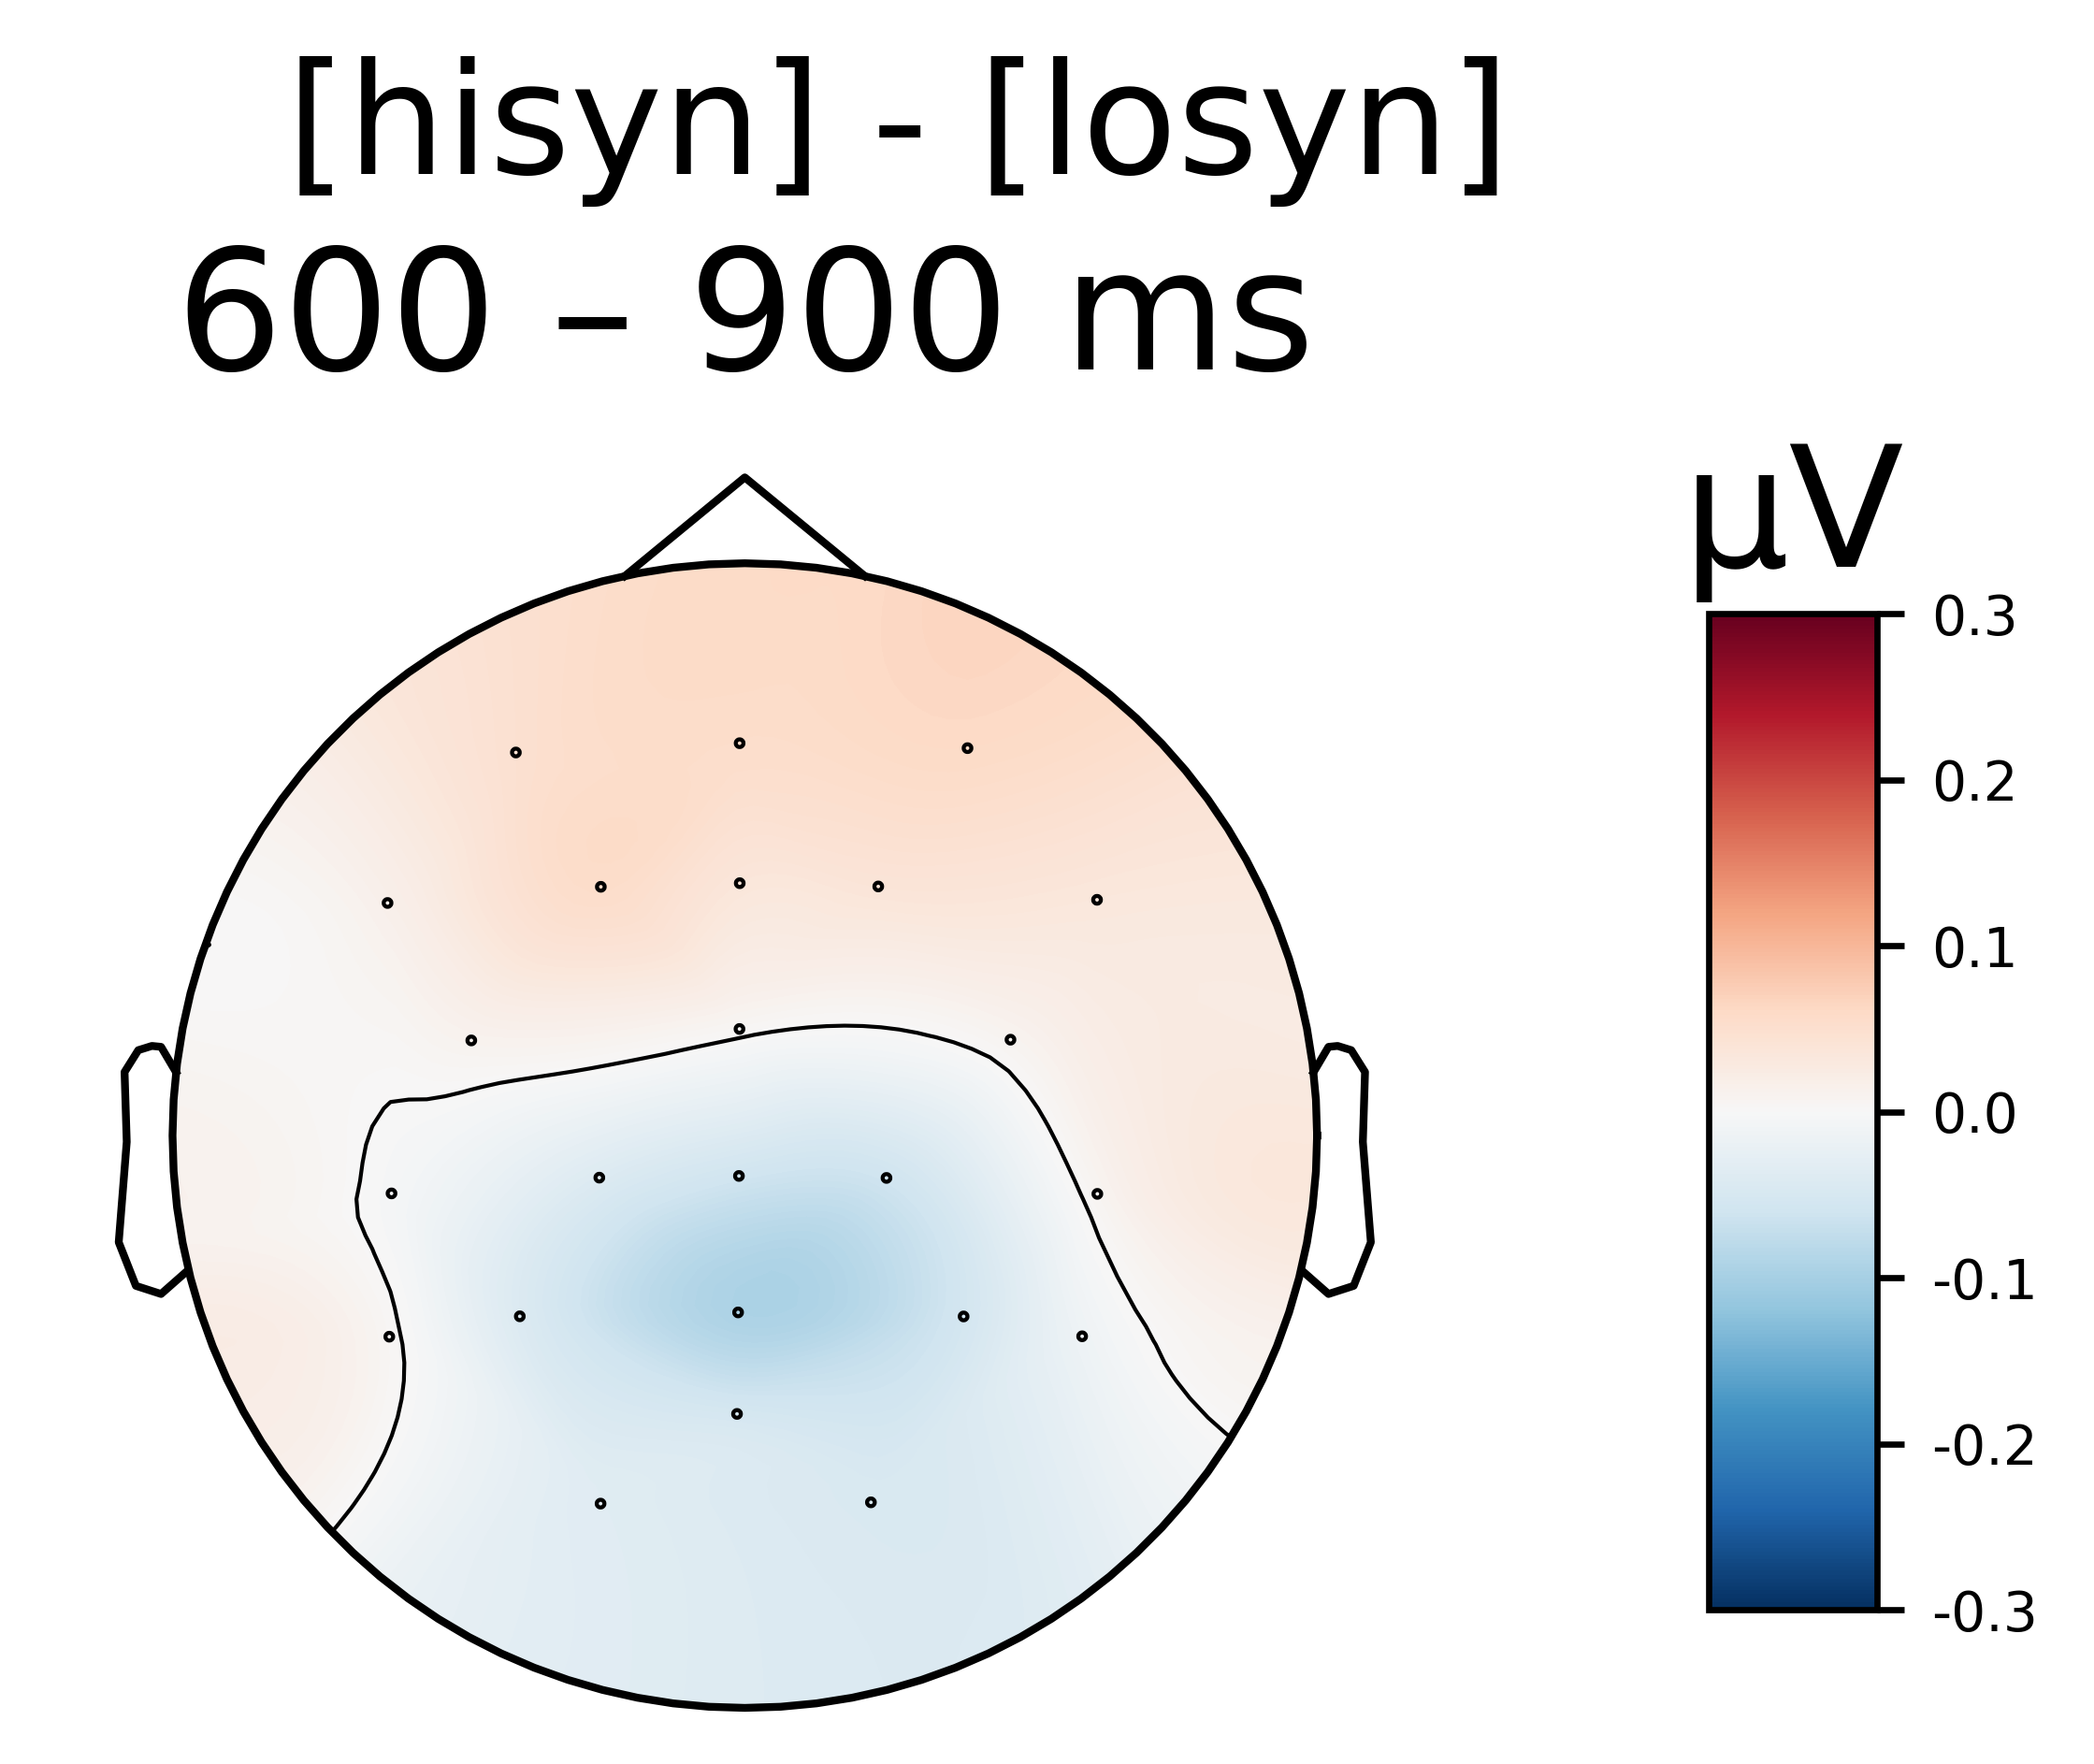
\includegraphics[scale=.65]{images/topo_subj-nsubj_600_900.png}}
\end{minipage}
\end{figure}

\paragraph{Hypothesis testing using Bayes factors}

Bayes factors are shown in Figure \ref{fig:eeg_bfs}. \Copy{ERP_results3}{\textcolor{blue}{In the N400 spatio-temporal window, the Bayes factors provided moderate to strong evidence for the semantic interference effect under all priors 
(Normal(0, 0.1): BF$_{10}$ = 6,
Normal(0, 0.5): BF$_{10}$ = 17.5,
Normal(0, 1): BF$_{10}$ = 9.4,
Normal(0, 2): BF$_{10}$ = 5). In the P600 spatio-temporal window, the Bayes factors provided anecdotal to moderate evidence (BF$_{10}$ between 2 and 4.3) for the semantic interference effect under priors assuming effects smaller than $\pm$1\,$\mu V$ and very weak evidence for it (BF$_{10}$ = 1.1) under priors assuming effects in the range of $\pm$2\,$\mu V$. By contrast, Bayes factors provided evidence against the syntactic interference effect in both spatio-temporal windows (BF$_{10}$ $<$ 0.9). The only exception was under the narrowest prior in the N400 window, there was very weak evidence for syntactic interference (BF$_{10}$ = 1.2). Similarly, Bayes factors provided evidence against the interaction in both spatio-temporal windows. The only exception was under the narrowest prior in the P600 window, there was very weak evidence for the interaction (BF$_{10}$ = 1.2). In sum, in our ERP data, there was decisive evidence for the semantic interference effect and mainly evidence against syntactic interference and the interaction.}}\label{ERP_results3}

\Copy{fig_bf_eeg}{
\begin{figure}[H]
    \caption{Bayes factors for the effects of semantic interference, syntactic interference and their interaction in the N400 (300 - 500 ms post critical verb onset) and P600 (600 - 900 ms post critical verb onset) time windows at centro-parietal electrode sites.}\label{fig:eeg_bfs}
    \centering
    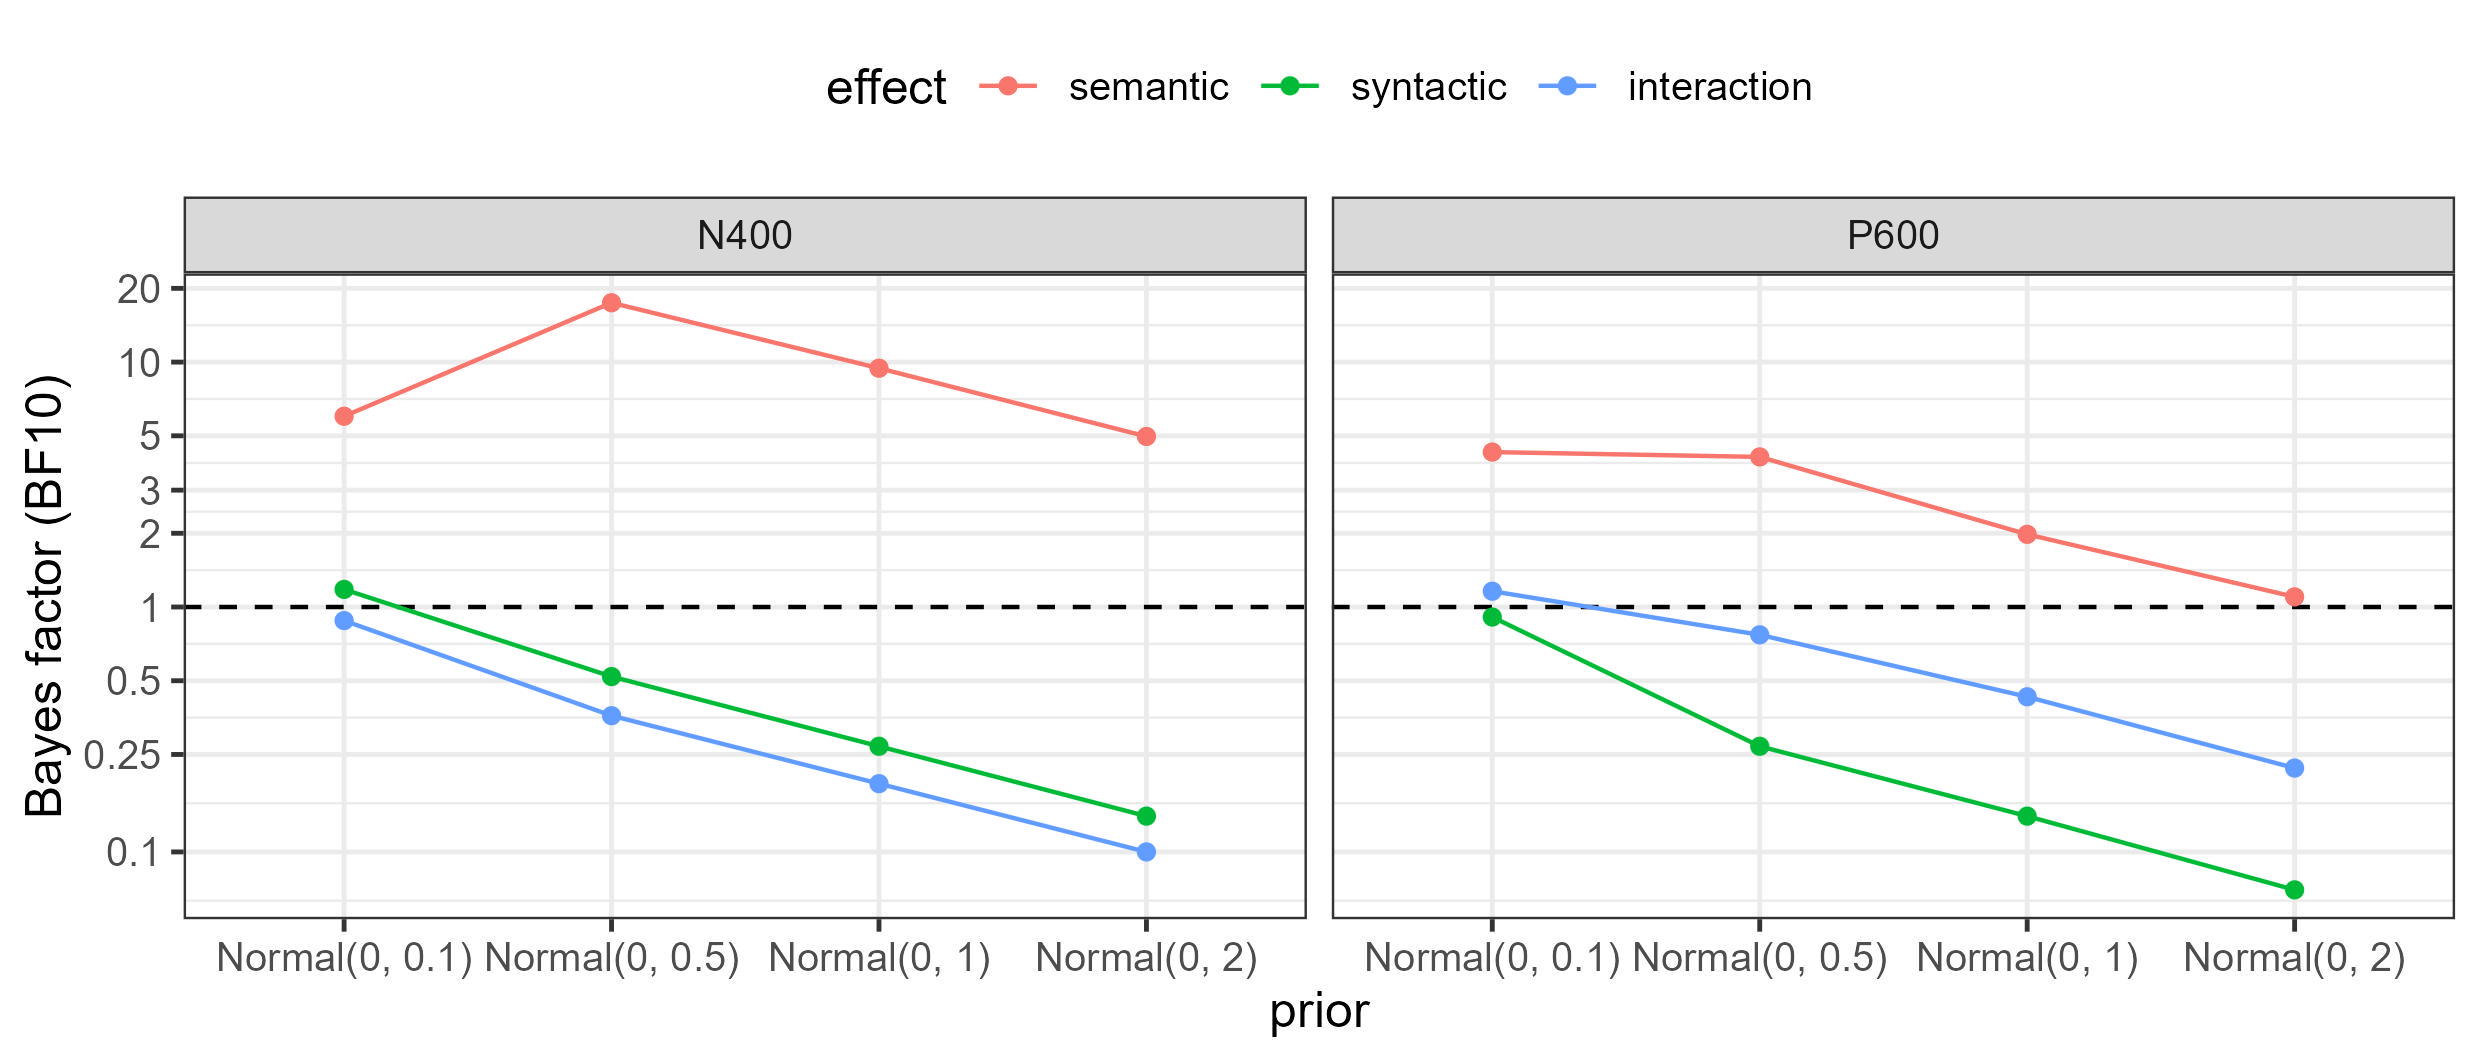
\includegraphics[width=1\textwidth]{images/BF_plot_eeg.jpg}
\end{figure} }



\subsection{Discussion}
We presented a large-scale ERP experiment investigating syntactic and semantic interference during subject-verb dependency completion. To our knowledge, this is the first ERP experiment on this classic interference design, which has only been investigated using reading studies so far \parencite{mertzen,vandyke07}. 

Comprehension accuracy was reduced for high vs.\ low semantic interference conditions. There was no indication that syntactic interference affected accuracy. The sign of the effect was in the expected direction, but  amounting to a 1\% difference on the probability scale between the high and low syntactic interference conditions. There was a numerical suggestion of an interaction: the difference in accuracy between low and high semantic interference conditions was larger when syntactic interference was high vs.\ when it was low (17 vs.\ 8 \% difference). 

\Copy{ERP_discussion}{The Bayes factors analyses found \textcolor{blue}{moderate to strong evidence for semantic interference in the N400 amplitude for the whole range of investigated effects sizes ($\pm$0.2 to $\pm4$\,$\mu V$). In the P600 spatio-temporal window, there was anecdotal to moderate evidence for semantic interference. Both the N400 and P600 were more negative under high vs. low semantic interference. In contrast, there was only very weak evidence for very small effects of syntactic interference and the interaction or even evidence against them in both the N400 and P600 windows. In sum, the ERP results showed clear evidence for semantic interference and mostly evidence against syntactic interference and the interaction of syntactic and semantic interference. Consequently, we conclude that the ERP data showed no syntactic interference and no interaction.}}\label{ERP_discussion}

Our finding that retrieval interference modulates the N400 amplitude supports the N400 as a marker of memory retrieval \citep{kutas&federmeier_2000, kutas_federmeier2011, brouwer2017_n4_p6, lau2008_n400}. The more complex memory retrieval under high semantic interference resulted in a more negative N400. \textcolor{blue}{This finding is in line with previous ERP studies on interference \citep{lee_garnsey, vasishth_drenhaus_2011, martinetal2014, schoknecht2022}. The semantic interference effect on the P600 is in the opposite direction than expected: High semantic interference lead to a reduced P600 amplitude compared to low semantic interference. Typically, the P600 amplitude is more positive when syntactic processing is complex, e.g., due to reanalysis \citep{osterhout&holcomb_1992}. The reduced P600 amplitude under high semantic interference in the present study might be explained by facilitatory interference \citep[see e.g.,][]{jaeger_etal_2017}. In the present design, subject-verb integration might be facilitated, i.e., easier, under high semantic interference because there are two semantically suitable candidates to act as the subject. A similar effect was found by \textcite{Tanner_etal_2017}. In their study, the P600 elicited by ungrammatical verbs which were incongruent in number was reduced when the sentence included a matching distractor. However, the present study investigated only grammatical subject-verb integration and the size of the P600 effect was rather small. The small size of the effect on average could indicate that the facilitation occurred only occasionally when the distractor was not ruled out during memory retrieval prior to integration. Since the Bayes factor analysis provided stronger support for the semantic interference effect in the N400 (largest BF$_{10}$ = 17.5) than in the P600 (largest BF$_{10}$ = 4.3), we focus on the N400 results in the remainder of this paper.}

Consistent with the self-paced reading study, there is clear evidence for semantic interference, and \textcolor{blue}{no evidence for syntactic interference in our ERP data}. How do these observed patterns compare to the theoretical predictions of cue-based retrieval theory? We turn to this point next by discussing the quantitative predictions of the \textcite{Lewis2005} model.

\section{Quantitative predictions of the Lewis and Vasishth (2005) model for \textcolor{blue}{ERPs elicited in} the present design}

\label{modeling}\Copy{modeling}{\textcolor{blue}{The \citet{Lewis2005} model is generally used to predict reading times. Recently, \textcite{mertzen} presented simulations for the present design that predicted approximately equally sized effects of syntactic and semantic interference in the reading times of the critical verb. We found that the reading times at the critical verb were confounded by pre-critical effects, which were best explained by \textit{encoding} interference. Because  Lewis and Vasishth (2005) model is a model of retrieval interference and not encoding interference, and because we cannot disentangle encoding and retrieval interference in the present design, it would not make sense to compare the results from the present SPR experiment to the model's predictions. However, the ERP data can be compared to the model's predictions; all that has to be changed is that the measurement is now on the microvolt scale instead of the millisecond scale. In order to model the ERP data, we therefore adjust the scaling factor $F$, which recales the activation of items in memory to the relevant dependent measure. The modeling reported here is, to the best of our knowledge, the first time that the \citet{Lewis2005} model has been fit quantitatively to ERP data. 

We sampled the free scaling parameter $F$ from a \textcolor{blue}{truncated normal prior distribution ($Normal_{lb=0,ub=0.05}(0.01, 0.01)$) with a lower bound of 0 and an upper bound of 0.05. This prior reflects the a priori belief that effect on the microvolt scale will range from 0 to 5 $\mu V$ with higher likelihood for effect sizes below 3 $\mu V$ (see Figure \ref{fig:model_predictions_ERP}). This relatively uninformative prior was chosen because although there exists no previously published ERP data on the Van Dyke (2007) design it reflects the reasonable range of effect sizes in psycholinguistic ERP research. In future work, the posterior distribution of the semantic interference effect in our ERP data, with range [-0.5, -0.1]\,$\mu V$, could be used as a basis for redefining a tighter prior on the scaling parameter $F$.} After sampling the scaling parameter, simulated data was generated from the model while holding all other parameters in the model at fixed values. \textcolor{blue}{We decided to model N400 amplitude differences because Bayes factors provided stronger evidence for the semantic interference effect on the N400 than on the P600 in the present ERP study. To reflect that larger predicted effect sizes correspond to more negative N400 amplitudes, the predicted effects from the model} were multiplied with $-1$.

\textcolor{blue}{For their recent simulations, \textcite{mertzen} created a version of the Lewis and Vasishth (2005) model that assumes that in the \textcite{vandyke07} design, three cues are used at the verb: \{$\pm$ animacy\}, \{$\pm$ grammatical subject\} and \{$\pm$ same clause\}. The \{$\pm$ same clause\} cue matches only with nouns that occurred in the same clause as the verb. ``The addition of the \{$\pm$ same clause\} cue [was] necessary to identify the correct subject'' and as a means for the model ``to achieve correct retrieval'' in the condition with high syntactic and high semantic interference \citep[][p. 14]{mertzen}. This model predicted approximately equally sized effects of syntactic and semantic interference. Although it is clear that our data does not support equally sized effects of syntactic and semantic interference, we decided to include their version of the model here because it has previously been claimed to be a good model for the present design. We have implemented two alternative versions of the model. Given the evidence against syntactic interference in our data, it is plausible that, at least in this experimental design and language, syntactic interference plays little to no role. We speculate that this could be due to the parser tracking hierarchical structure and that this hierarchical information is used when searching for a noun in memory -- even more so than suggested by \textcite{mertzen}.} \Copy{clause_tracker}{\textcolor{blue}{So, we implemented a model which puts even more emphasis on hierarchical syntactic structure and thereby basically eliminates syntactic interference.} Specifically, the relevant syntactic cues that might be used at the verb are not \{$\pm$ grammatical subject\} and \{$\pm$ same clause\} -- as implemented by \textcite{mertzen} -- but rather a composite cue \{$\pm$ subject-in-same-clause\}. \textcolor{blue}{As already noted by \textcite{mertzen}, structural information like [+ subject of clause$_i$] is not an inherent feature like for example [+ animate], but within in the cue-based retrieval framework, we can easily assume that such a feature is encoded into memory and can consequently be used to match the retrieval cue \{$\pm$ subject of clause$_i$\}. This idea goes back to the roots of the Lewis and Vasishth (2005) model by making the model ``sensitive to whether or not it is parsing an embedded clause'' \citep[][p.388]{Lewis2005} and entails a simple clause tracking mechanism.} The resulting model assumes two retrieval cues: \{$\pm$ subject-in-same-clause\} and \{$\pm$ animate\}. This proposal is \textcolor{blue}{furthermore} in the spirit of the \textcite{dillon2013} and \textcite{Sturt2003} claim, that the parser intelligently targets only the syntactically relevant noun during antecedent retrieval. In the present case, it is possible that syntactically relevant noun is only the one in the same clause as the verb. \textcolor{blue}{For more discussion of the role of structural retrieval cues, see \textcite{franck2020hierarchical} and \textcite{arnett2017subject}.}}\label{clause_tracker} \textcolor{blue}{The here proposed model using two cues predicts no syntactic interference and no interaction, but semantic interference effects. Lastly, we implemented a model with one cue which unambiguously matches the subject. This cue would be the master composite cue \{$\pm$ animate-subject-in-same-clause\}. This model naturally does not predict any interference effects. It can be regarded the null model or no-interference model.}
 
\textcolor{blue}{Figure \ref{fig:model_predictions_ERP} shows the  prior predictive distributions of the effects of interest for the three competing models discussed above in comparison to our ERP data.  The null model model using one cue predicts no interference effects. The new two-cues model, including a syntactic cue that utilizes syntactic hierarchy, predicts no effect of syntactic interference and no interaction, but a semantic interference effect. The prior predictions from the three-cues model show equally large effects of syntactic and semantic interference and an interaction. The predictions of all models overlap with the effects of interest in the data. }

\Copy{fig:model_predictions_ERP}{
\begin{figure}[htpb]
    \caption{The prior predictions on the microvolt scale for syntactic and semantic interference and their interaction \textcolor{blue}{from three versions of the Lewis and Vasishth (2005) cue-based retrieval model.}
    %using the two cues \{$\pm$ subject-in-same-clause\} and \{$\pm$ animate\}. 
    The data with 95 \% credible intervals are shown in red.}\label{fig:model_predictions_ERP}
        \centering
         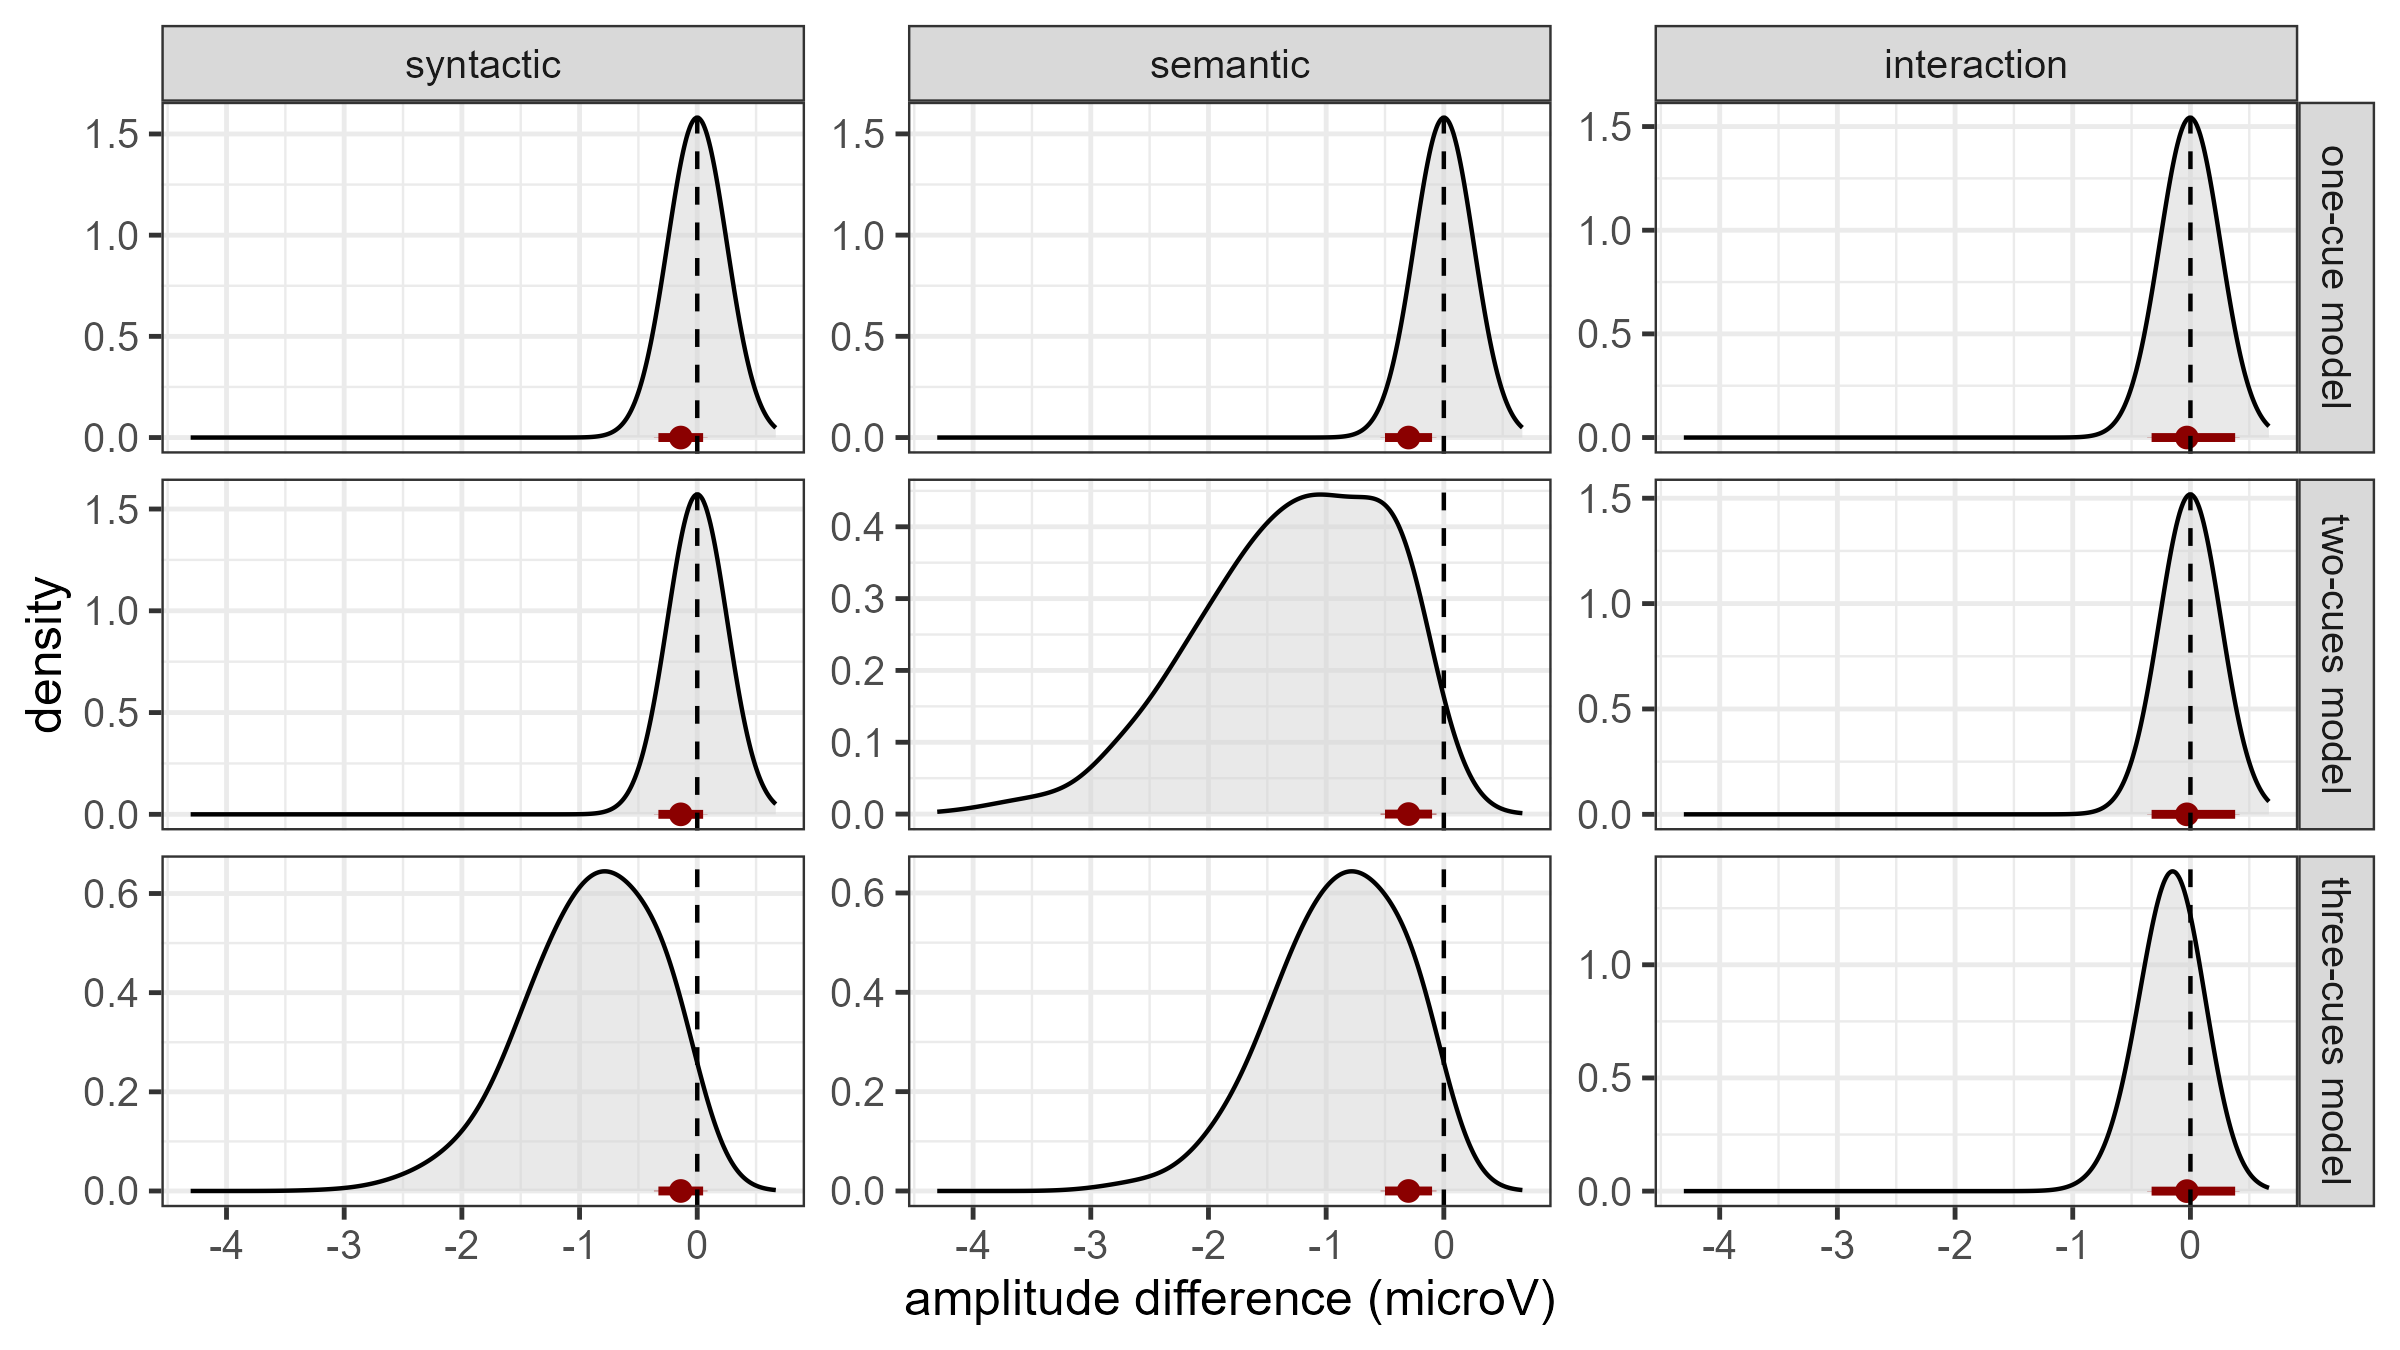
\includegraphics[width=\textwidth]{images/compmod_predictions.png}
\end{figure}
}

\textcolor{blue}{To quantitatively evaluate the relative predictive performances of the models on the semantic interference data, we used a Bayes factor analysis. We computed Bayes factors for the two-cues model compared to the three-cues model and to the one cue model, respectively. Since Bayes factors are sensitive to the choice of priors on the parameters of interest, we computed Bayes factors under six different priors for the latency factor parameter $F$,
$Normal$(0.01,0.01), 
$Normal$(0.01,0.02),
$Normal$(0.01,0.005),
$Normal$(0.02,0.01),
$Normal$(0.02,0.02), and 
$Normal$(0.02,0.005). }

\textcolor{blue}{The procedure for computing Bayes factors is described as follows. The Bayes factor computation required us to estimate the marginal likelihood of the competing models. We used the Monte Carlo integration method to estimate the marginal likelihood of each model. First, we chose an importance density for the parameter $F$ from which we draw $0.2$ million samples of $F$. Then, for each of these proposed parameter values, we compute the likelihood and prior density. The estimated marginal likelihood of a model will be given by}

\begin{equation}
ML = \frac{1}{n} \sum_{i=1}{n} \mathcal{L}{F_i|y} p(F_i)  \text{ where } F_i \sim Normal_{lb=0,ub=0.05}(0.0.025) 
\end{equation}

\noindent \textcolor{blue}{where $y$ is the observed data, i.e., the observed semantic interference effect in our case, $F_i$ is the $i^{th}$ proposal from the importance density $Normal_{lb=0,ub=0.05}(0.0.025) $. The term $\mathcal{L}{F_i|y}$ gives the likelihood of proposal $F_i$ given the data $y$ and $p(F_i)$ gives the prior density of $F_i$. We compute marginal likelihoods under different prior assumptions $p(F)$.}

\textcolor{blue}{The Lewis and Vasishth (2005) model is a complex, non-deterministic model and it is difficult to express the model's likelihood analytically without drastically simplifying the model \parencite[e.g., in][]{NicenboimRetrieval2018,lisson2020computational}. In absence of an analytically-expressed likelihood function, we used an Approximate Bayesian Computation (ABC)~\citep{sisson2018handbook,palestro2018likelihood} approach to estimate approximate likelihood for a given value of $F$. Under this approach, we compared the model generated data conditioned on $F=F_i$ and the actual observed data $y$. If the model-generated data $x_{i} \sim Model(F_i)$ for $F_i$ was close to the actual data $y$, then $F_i$ has higher likelihood and vice versa. The likelihood term can be rewritten as $\mathcal{L}{F_i|y} = \Psi(d(x_i, y), 0 , \delta)$, where $\Psi(.|\delta)$ represent a density kernel that weighs a proposal $F_i$ based on distance between model-generated data and actual data, $d(x_i,y)$.}

\textcolor{blue}{From the marginal likelihoods, we computed Bayes factors for the two-cues model compared to the three-cues model and the one-cue model. That is, the marginal likelihood of the two-cues model $M_1$ was divided by the marginal likelihood of the three-cues model $M_2$ and one-cue model $M_3$ to obtain the Bayes factors $BF_{12}$ and $BF_{13}$, respectively. Following the convention from \textcite{jeffreys1998theory}, a Bayes factor above 10 is interpreted as strong evidence in favor of the two-cues model and a value between 3 and 10 is interpreted as moderate evidence in favor of the two-cues model compared to the competing model (see also Table \ref{tab:bf_interpretation}).}

\textcolor{blue}{The Bayes factors under different priors on $F$ are shown in Figure \ref{fig:BF_compmods}. Compared to the null model, the one-cue model, the Bayes factors indicate strong evidence for the new two-cues model. Therefore, we can conclude that the computational modeling shows that our data shows interference. Compared to the three-cues model proposed by \textcite{mertzen}, the Bayes factors provide moderate evidence for the new two-cues model. Therefore, the assumption that the relevant syntactic cue is the \{$\pm$subject-in-same-clause\} cue – rather than the previously assumed \{$\pm$grammatical subject\} cue – is moderately supported by these modeling results. This result holds for prior assumptions that allows higher probability mass for small values of $F$., i.e., for $F<0.01$.}

\begin{figure}
    \centering
    \caption{Comparison of the predictive accuracies of the three versions of the Lewis and Vasishth (2005) cue-based retrieval model on our ERP data. The facets show how the new two-cues model performs compared the the three-cues model and the one-cue model, respectively. Larger Bayes factors correspond to better performance of the two-cues model.}
    \label{fig:BF_compmods}
    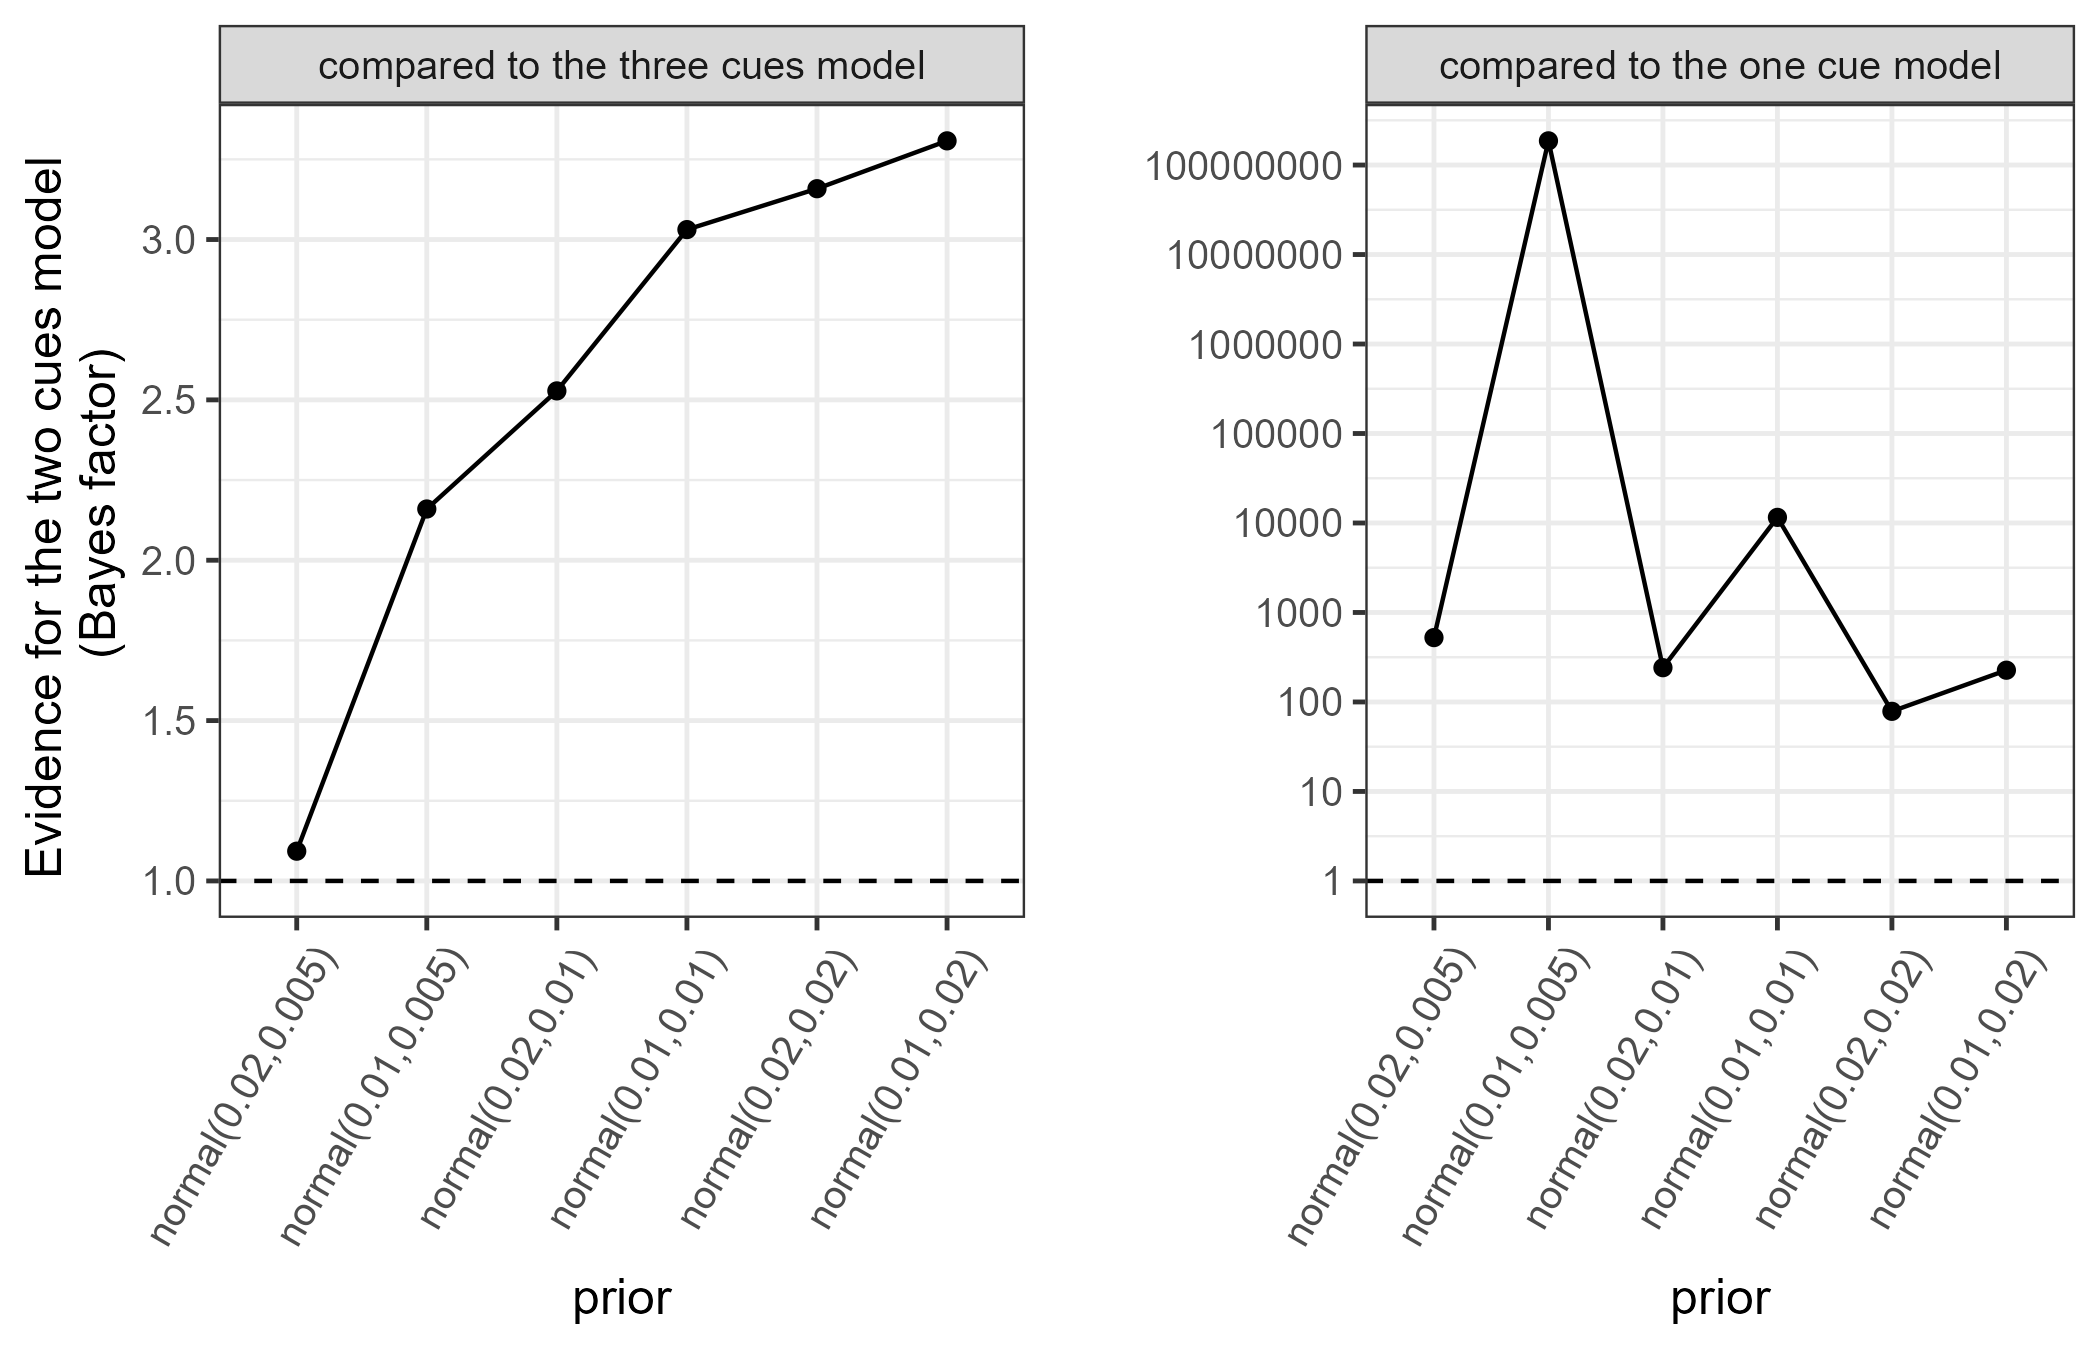
\includegraphics[width=\linewidth]{images/BF_plot_compmodels.png}
\end{figure}

Thus, the theoretical assumption that is consistent with the observed ERP data is that although the parser uses the animacy cue exactly as proposed in previous work on cue-based retrieval, the syntactic cue keeps track of the clausal location of the subject. This is of course a speculative claim that would need to be further investigated empirically. 

}%end copy

\section{General discussion}

\Copy{only_this_design}{Taken together, the SPR and ERP experiments \textcolor{blue}{using the 2 $\times$ 2 interference design developed by \textcite{vandyke07}} consistently showed effects of semantic interference and no effects of syntactic interference \textcolor{blue}{or an interaction}.}\label{only_this_design} This pattern was not only found in the dependent measures of the experiments that were of primary interest, but also in the comprehension accuracy. 
The modeling reported here suggests that one way to explain the observed pattern in the context of cue-based retrieval is to assume the following: the parser searches for a subject that is within the same clause, but uses the animacy cue without reference to the clause that a noun appears in. A broader implication is that the human sentence comprehension system may be using the hierarchical syntactic structure to selectively target nouns for retrieval; this is an idea that has independent support in the literature \citep[e.g.,][]{Sturt2003,dillon2013,yadav2021individual}.

\textcolor{blue}{In the remainder of this section, we first provide an in-depth comparison of the present results to the previous studies' results which used the same design. Then we discuss two important issues that relate to the broader interference literature}. The first is the role of encoding vs.\ retrieval interference, and the second is broader implications of our findings in the context of previous related work.

\subsection{\textcolor{blue}{Comparison with previous findings}}\label{comparison}
\Copy{comparison}{\textcolor{blue}{The present study used the same design as two previous studies \parencite{vandyke07, mertzen}. Figure \ref{fig:previous_vs_present} A shows the estimated reading times differences from the previous studies and the present self-paced reading experiment. Because the \textcite{vandyke07} data was not available to us, we derived estimates for their study from the summary statistics in the published paper. \textcite{mertzen} made their data available. In comparison to the previous estimates, the effects of the present study are relatively small and associated with less uncertainty in general. The present and previous estimates of semantic interference seem relatively consistent: They indicate a positive effect which is largest in the pre-critical region and smallest in the critical region. It seems like the present estimates of syntactic interference are smaller, i.e., closer to zero, than the previous estimates. For the interaction, the present estimates are larger, i.e., further from zero in the positive direction, than the previous ones. To see whether there is evidence for the estimated effects, we computed Bayes factors for the previous studies to compare them to the present Bayes factors. For maximal comparability, we used only the self-paced reading times and total fixation times from the previous studies for this comparison. To compute Bayes factors for \textcite{vandyke07}, we used the Normal-Normal conjugate case to derive posteriors from the summary statistics (mean and SE) in the published paper. Then, using these posteriors and a reasonable prior (Normal(0,0.5), a priori assumed effect size in the range of -40 ms to 40 ms), we computed Bayes factors with the Savage-Dickey method. Bayes factors for \citeauthor{mertzen}'s (\citeyear{mertzen}) data were computed using the Savage-Dickey method from hierarchical mixed models which we run on their data analog to our own analyses described in Statistical Analyses for Experiments 1a and b. The Bayes factors for the effects of interest of the present and previous studies under prior Normal(0,0.5) are shown in Figure \ref{fig:previous_vs_present} B.}

\begin{sidewaysfigure}[h]
    \caption{A) Reading time differences in the regions of interest from the present and previous studies using the design by \textcite{vandyke07}. VD07.E1, VD07.E2 and VD07.E3 stand for \citeauthor{vandyke07}'s (\citeyear{vandyke07}) Experiments 1-3. The intervals for \citeauthor{vandyke07}'s (\citeyear{vandyke07}) estimates are 95\% confidence intervals. M23.E and M23.G stand for \citeauthor{mertzen}'s (\citeyear{mertzen}) English and German experiment, respectively. The intervals for their study and the present study are Bayesian 95\% credible intervals. There are less estimates for the pre-critical region because \citeauthor{vandyke07}'s (\citeyear{vandyke07}) Experiment 1 and 2 did not have a pre-critical region. B) Bayes factors for the effects of interest in the present and previous studies under prior Normal(0,0.5).}
    \label{fig:previous_vs_present}
    \centering
    \includegraphics[width=0.9\linewidth]{images/present_previous_allplots.jpg}
\end{sidewaysfigure}
\clearpage

\textcolor{blue}{In the pre-critical region, the Bayes factors from the present and previous studies showed no clear pattern regarding syntactic interference. The present study was the only one to provide evidence against the effect, while the previous studies supported it. The Bayes factors aligned qualitatively across studies for the semantic interference effect and the interaction -- consistently providing evidence for semantic interference and against the interaction.}

\textcolor{blue}{In the critical region, the Bayes factors across studies showed a mixed picture for syntactic interference: \citeauthor{vandyke07}'s (\citeyear{vandyke07}) Experiment 2 provided extremely strong evidence for it, while \citeauthor{vandyke07}'s (\citeyear{vandyke07}) Experiment 3 provided weak evidence against it. \citeauthor{mertzen}'s (\citeyear{mertzen}) experiments showed weak evidence for the effect. The two self-paced reading experiments provided evidence against it. Similarly, there is no clear pattern for semantic interference: Most experiments provided evidence against it, but the two self-paced reading experiments (present and \citeauthor{vandyke07}'s (\citeyear{vandyke07}) Experiment 1) provided evidence for semantic interference. The Bayes factors across studies provided evidence against the interaction.}

\textcolor{blue}{In the spill-over region, the Bayes factors for syntactic interference rather consistently provided evidence against the effect. Only \citeauthor{mertzen}'s (\citeyear{mertzen}) English experiment provided moderate evidence for it. The Bayes factor results for semantic interference were mixed: the two self-paced reading experiments provided extremely strong evidence for the effect, two of the eye-tracking experiments (\citeauthor{vandyke07}'s (\citeyear{vandyke07}) Experiment 3, \citeauthor{mertzen}'s (\citeyear{mertzen}) German experiment) provided weak evidence for the effect and the two other eye-tracking experiments (\citeauthor{vandyke07}'s (\citeyear{vandyke07}) Experiment 2, \citeauthor{mertzen}'s (\citeyear{mertzen}) English experiment) provided evidence against the effect. Importantly, the clustering in the results did neither align with the investigated language nor with the authors of the studies. The Bayes factor results for the interaction showed evidence against it from all experiments but one. The outlier was \citeauthor{vandyke07}'s (\citeyear{vandyke07}) SPR experiment, which showed extreme evidence for the interaction.}

\textcolor{blue}{In sum, while the present and previous studies mostly showed comparable region-wise results for semantic interference and the interaction, they differed remarkably regarding syntactic interference in the pre-critical and critical region. In the pre-critical region, the present study was the obvious outlier, being the only study to provide evidence against the effect. In the critical region, the Bayes factors for the syntactic interference were very mixed with no clear clustering. In conclusion, the most remarkable difference between the present study and previous findings concerns syntactic interference in the pre-critical region. The lack of syntactic interference in the pre-critical region in the present study compared to the previous studies could be explained by differences in i) methodology, ii) items and/or iii) statistical power. We discuss each of these differences in turn.}
}

An obvious difference between the studies is the experimental methodology. The majority of the previous experiments employed eye-tracking while reading, while we used self-paced reading \textcolor{blue}{and EEG / ERPs. However, word-by-word} self-paced reading (SPR) \textcolor{blue}{and ERPs elicited by single words presented in the typical rapid serial presentation (RSVP) format, if anything} might have a greater tendency to be affected by interference compared to natural reading (as in eye-tracking studies), due to the restricted reading format: Comprehenders have no opportunity to revisit previous material during conventional self-paced reading \citep[but see][]{BSPR} \textcolor{blue}{and RSVP. Word-by-word presentation} is likely to be more demanding on the comprehender's memory, which \textcolor{blue}{should} make it easier to detect interference effects. \textcolor{blue}{So, the differences in methodology do not offer a straightforward explanation for the lack of syntactic interference in our data compared to the previous studies.}

\Copy{linebreak}{\textcolor{blue}{The difference in methodology lead to another difference between our study and the previous studies. In their eye-tracking experiments, \textcite{vandyke07} and \textcite{mertzen} presented the stimuli on a single line. Whether \citeauthor{vandyke07}'s (\citeyear{vandyke07}) SPR experiment used line breaks or not is not reported. In our SPR experiments, it was necessary to introduce line breaks. These were hard-coded to occur always after the subject of the critical verb and two words after the critical verb. The line break after the subject might have increased its prominence compared to the other nouns in the sentence, i.e., the distractor. It has been proposed by \textcite{engelmann_etal_2019} that prominence within the current context increases the activation of a memory representation which leads to faster retrieval and higher retrieval probability. Therefore, increased prominence of the subject could have decreased interference. Since we have found evidence for semantic, but not for syntactic interference, the increased prominence might have especially affected syntactic interference. For this point to hold, one would need to make the reasonable assumption that the line break provided additional structural information by emphasizing the syntactic structure of our sentences. However, our EEG experiment used word-by-word presentation for all words, so there was no additional structural information which might have increased the prominence of the subject compared to the distractor. So, the line break might have decreased syntactic interference in our SPR experiments, but not in the EEG experiment. Nevertheless, both the SPR and the EEG experiment showed predominantly evidence against syntactic interference.}
}\label{linebreak}

\textcolor{blue}{We now turn to the differences regarding the experimental items. The three studies investigating syntactic and semantic interference with the same design used either English or German items. Cue-based retrieval as a theory on the memory processes during sentence comprehension implicitly states that these memory processes do not differ cross-linguistically \citep{lewis06, Lewis2005}. This is in line with no apparent clustering of the English vs.\, German results (see Figure \ref{fig:previous_vs_present} A). So, the use of materials in different languages cannot account for the differences in results between the studies.}

\textcolor{blue}{The previous and present items differed in the pre-critical material. \citet{vandyke07} used one region consisting of two words (e.g., `yesterday afternoon') which were analyzed together. \textcite{mertzen} used a one-word pre-critical region (e.g., `tatsächlich', indeed). In the present study, we added a pre-pre-critical region to help us differentiate between the potential sources of the pre-critical effects in the literature as discussed in the Discussion of the SPR experiments. So, the present study was the only one which had a pre-critical region that did not directly follow a clause boundary and it was also the only one to not find syntactic interference in the pre-critical region. These two observations combined suggest that the pre-critical syntactic interference effect in the previous studies might be a spill-over effect from the syntactic manipulation. The syntactic interference manipulation in all the studies using this design was confounded with syntactic complexity of the material intervening between the subject and the (pre-)critical region. In the low syntactic interference conditions, it was a simple relative clause (who VP PP). In the high syntactic interference conditions, it was a relative clause with an embedded complement clause (who VP that NP VP). This difference in syntactic complexity could have ``spilled over'' into the pre-critical region of the previous studies causing the syntactic (interference) effect. While this seems like a plausible explanation for the previous effects, it would also apply to our pre-pre-critical region. However, Figure \ref{fig:whole_sentence} C shows that the pre-pre-critical region (n-2) in our items did not show a syntactic effect.}

\Copy{comma}{\textcolor{blue}{Another item-related difference is that all our experiments (SPR and EEG) displayed the subject with a comma. Commas are mandatory in German to separate subordinate clauses from the main clause. Similar to the line break discussed above, the comma could have emphasized the syntactic structure of the sentences and therefore decreased syntactic interference from the distractor which occurred in another clause than the critical verb. But if this comma provided information about the syntactic structure of the items then it should have done so in \citeauthor{mertzen}'s (\citeyear{mertzen}) German study as well because they also presented the subject with a comma. But \citet{mertzen} found syntactic interference and we did not. So, while it is plausible that commas provide structural information, it cannot explain the difference in findings between our study and the previous studies.}}\label{comma}

The contrast between our results and those from  \citeauthor{mertzen}'s (\citeyear{mertzen}) German experiment is surprising given that both used German items and partially even the same linguistic material. \Copy{items_mertzen}{\textcolor{blue}{However, \citet{mertzen} changed the structure of the relative clause modifying the subject by adding an additional animate distractor to all conditions (see an example of one of their English items in \ref{ex:mertzen}; their items had this structure cross-linguistically). This was done to ``increase the strength of the manipulation.'' \citep[][p. 9]{mertzen}. }

\begin{exe}[ht]
\ex \label{ex:mertzen} 
\textcolor{blue}{It turned out that the attorney whose secretary had forgotten that the visitor was important frequently complained about the salary at the firm. \parencite{mertzen}}
\end{exe}
}

\textcolor{blue}{The additional distractor (`the secretary' in \ref{ex:mertzen}) was animate and the subject of the relative clause, therefore theoretically it should have affected both syntactic and semantic interference equally. But it is possible that it increased syntactic interference in \citeauthor{mertzen}'s (\citeyear{mertzen}) experiment to a larger extent because the additional distractor (`the secretary') was a ``stronger'' subject than the manipulated distractor (`the visitor') because it was the subject of a full finite verb while the latter was always the subject of verb phrase consisting of an auxiliar and an adjective. This additional distractor might have increased syntactic interference compared to our study. But it would have increased syntactic interference in comparison to \citeauthor{vandyke07}'s study as well and this was not the case (see Figure \ref{fig:previous_vs_present} A).}\label{items_mertzen} \textcolor{blue}{All in all, differences in the items provide no clear explanation why the previous studies found syntactic interference and the present study did not.}

\textcolor{blue}{A plausible explanation for the divergence between studies is a difference in statistical power:} The present study has higher statistical power than the previous studies. \citet{vandyke07} had 35 - 40 participants and 36 - 48 items in each of her three experiments, respectively. \textcite{mertzen} tested 61 English speakers and 121 German speakers with 40 items each. In contrast, \textcolor{blue}{in our SPR experiments,} we tested 774 participants with at least 60 items each (a subset of 160 participants read all 120 items). Therefore, the present study is the study with the highest power to date using this 2 $\times$ 2 interference design. Consequently, the estimates from the present study are the most precise ones so far for this design. \textcolor{blue}{This is reflected by the tighter estimates in Figure \ref{fig:previous_vs_present} A}. The smaller effect size in the present study is a consequence of higher power, and the magnitude of the effects observed is comparable to that of other large-scale reading studies \citep{nicenboim} and meta-analyses on interference \citep{jaeger_etal_2017}. \textcolor{blue}{In contrast, the large estimates of the previous studies are likely Type M errors, i.e., exaggerations, which are common in low-powered studies \parencite{gelman_carlin}. That at least some of the previous studies had low power is further emphasized by the large uncertainty associated with some of the previous estimates (see Figure \ref{fig:previous_vs_present} A).}

\textcolor{blue}{In sum, while there are differences in the employed methodology and items between the present and previous studies, the most likely cause of the different results is the difference in statistical power. However, an alternative explanation could be that syntactic interference might differ inter-individually \parencite{yadav2021individual} and that the previous studies by chance sampled disproportionally many participants who showed syntactic interference, while we by chance sampled participants who did not.} 

\Copy{not_an_anomaly}{\textcolor{blue}{While it seems unfortunate that the present and previous results together do not create a clear and unambiguous picture of the investigated phenomena, this divergence of results is not an anomaly within the scientific literature \citep[see e.g.,][for a high-powered failed replication attempt of a classic result in the area of predictive processing]{nieuwland_etal_2018}. The only way to resolve contradictions in the literature -- like the contradictory results between the present and previous studies regarding syntactic interference -- is by carrying out adequately powered studies in the future to reach consensus over time.}}\label{not_an_anomaly}

\subsection{Encoding and retrieval interference}
In the SPR data, we found that the semantic interference effect originated at the distractor and persisted throughout the following regions. Due to this time course, encoding interference \parencite{Yadavetal2022,hammerly2019grammaticality} is the best explanation for the interference effect\textcolor{blue}{s in our SPR data}. This raises the question whether the ERP effect was also caused by encoding interference, i.e., whether the ERP effect originated prior to the critical region. To answer this question, it is necessary to look at the ERPs elicited by words earlier in the sentence, This is an unusual step in ERP research but makes sense as an exploratory step in the present context. 

Figure \ref{fig:erp_precrit} shows the ERPs for all conditions at the critical word and the two pre-critical adverbs which were identical across conditions. It is apparent from the ERPs of the pre-pre-critical and pre-critical word that the semantic interference effect found at the critical verb was not present at the words preceding it. 

\begin{figure}[H]
    \caption{ERPs elicited by the pre-pre-critical adverb (word onset at -1800 ms), pre-critical adverb (word onset at -900 ms) and critical verb (word onset at 0\,ms) at electrode Cz.}
    \label{fig:erp_precrit}
    \centering
    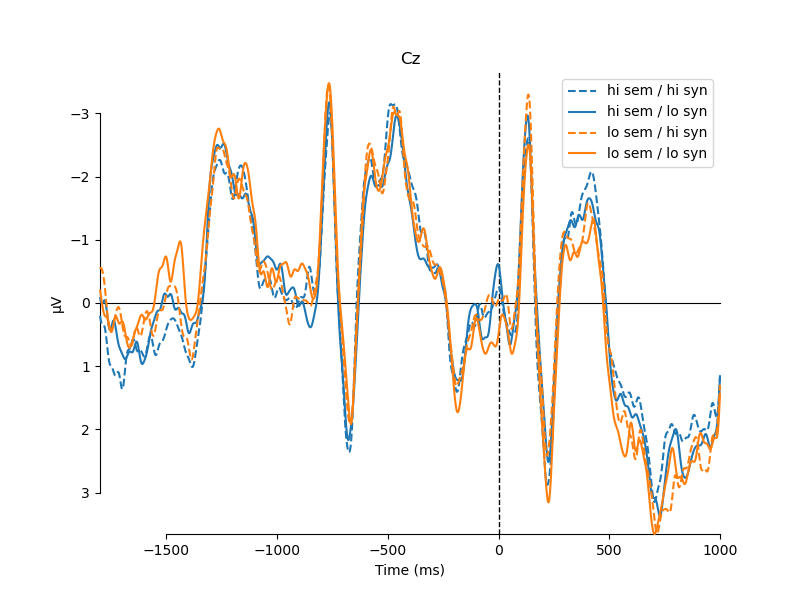
\includegraphics[width=0.95\textwidth]{images/N_103_Cz_precrit.png}
\end{figure}

Thus, the words directly preceding the critical verb do not show a pattern consistent with semantic interference. A further question that arises is: which brain response was elicited by the distractor itself (see Figure \ref{fig:erp_distractor})? An exploratory visual inspection of the ERPs elicited by the distractor shows several differences between conditions, but no semantic interference effect in the N400 spatio-temporal window. 

We believe that the differences in the ERPs elicited by the distractor in the different conditions are caused by two factors. First, the high and low syntactic interference conditions have different word orders, i.e., the distractors are embedded in different phrase structures (simple noun phrase vs.\ noun phrase including an adjective within a prepositional phrase; see Example \ref{ex:materials}). This is also apparent from the large difference between high and low syntactic interference conditions before distractor onset. Second, the distractors were not identical across conditions; therefore, the ERPs in Figure \ref{fig:erp_distractor} are elicited by different words in the high vs.\ low semantic interference conditions. In summary, this exploratory analysis suggests that the distractors did induce different brain responses across conditions, but these could be due to factors other than encoding interference. More importantly, these effects did not linger throughout the rest of the sentence (see Figure \ref{fig:erp_precrit}). 

\begin{figure}[H]
    \centering
        \caption{ERPs elicited by the distractor (word onset at 0 ms) at eight selected electrodes.}
    \label{fig:erp_distractor}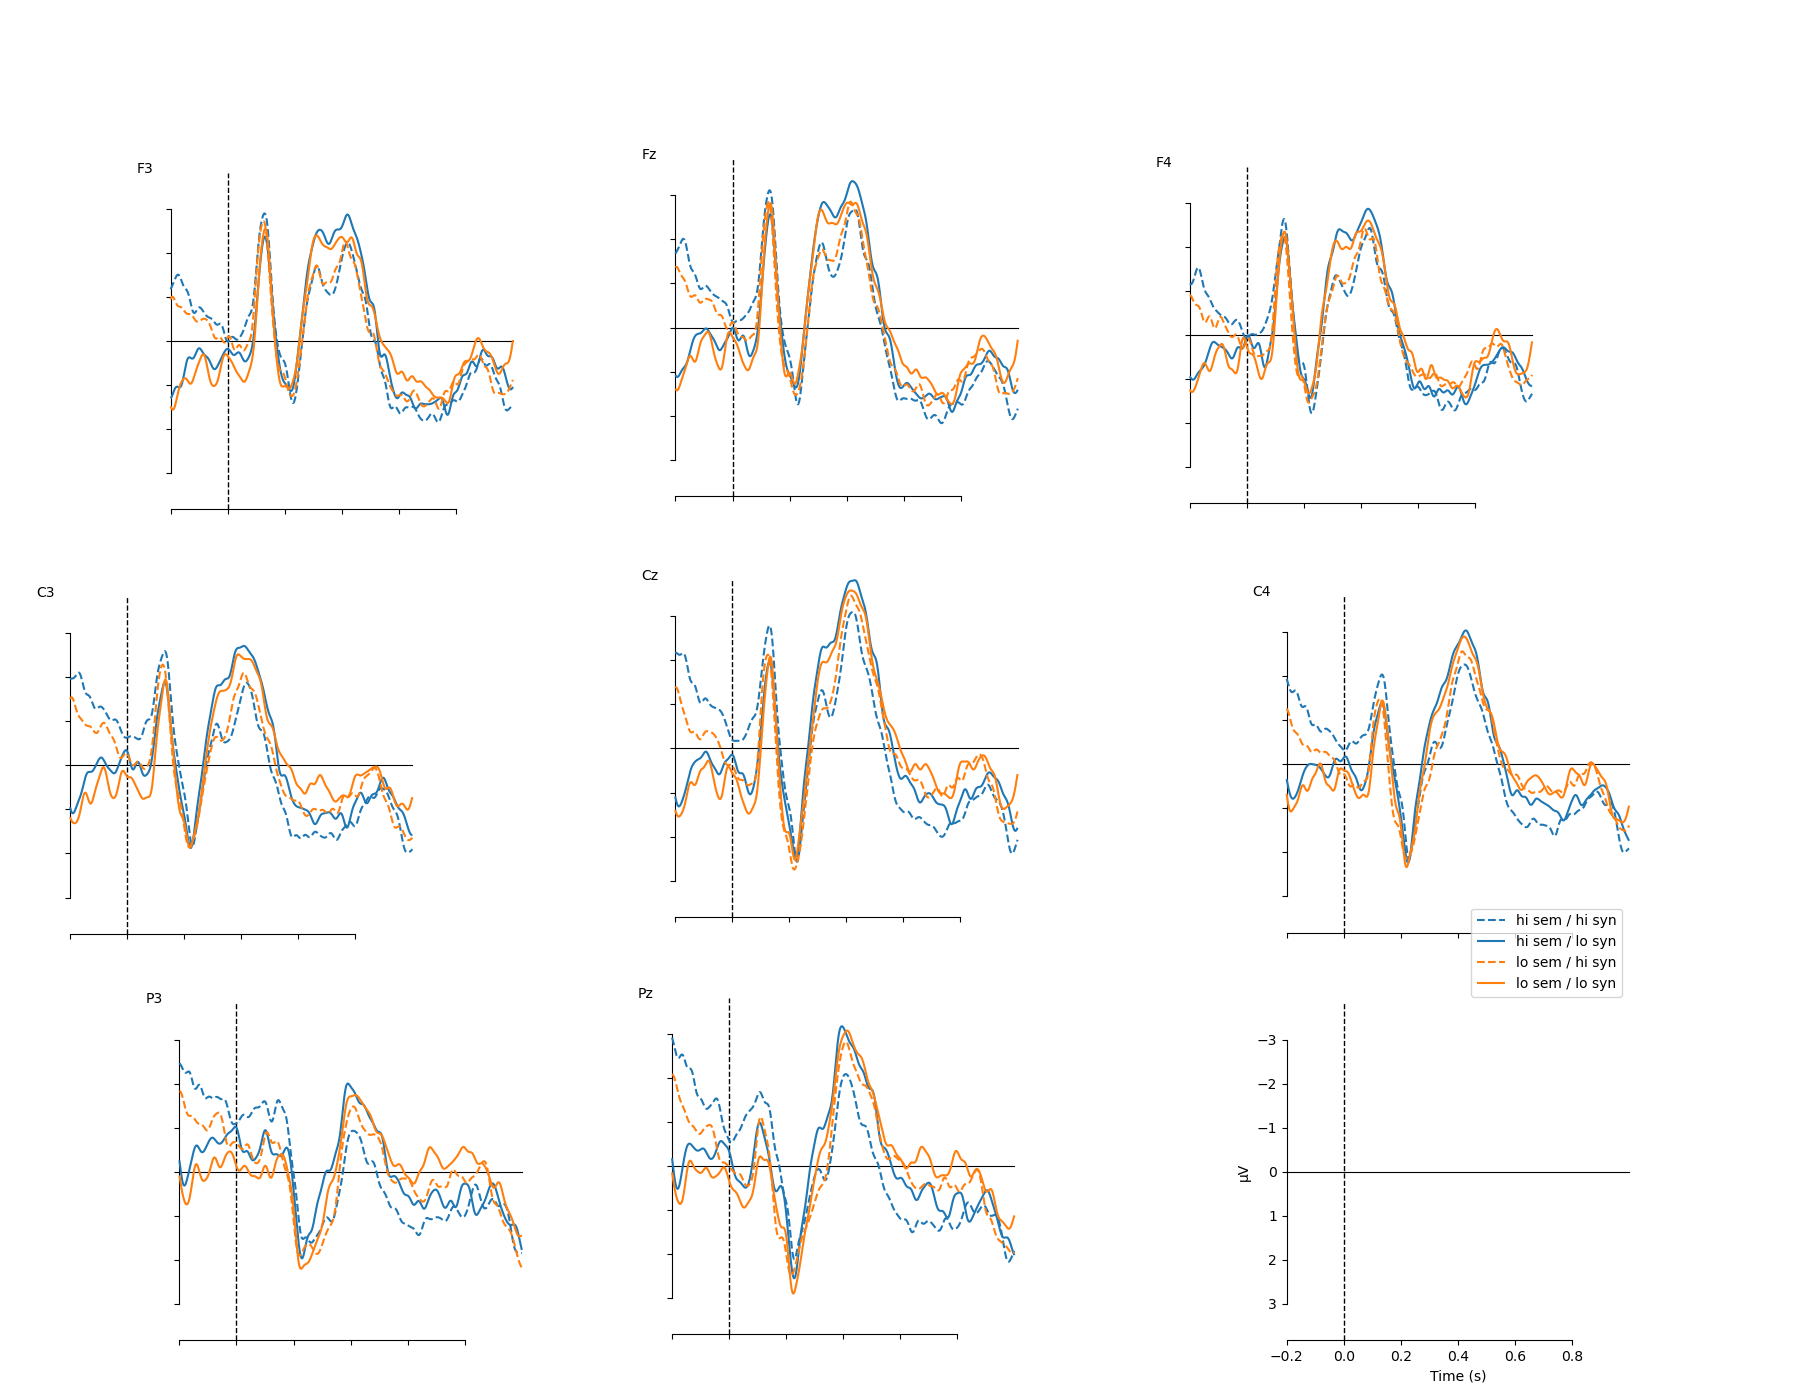
\includegraphics[width=\textwidth]{images/Distractor_N_100_some_elec.png}
\end{figure}

The comparison of the results of our SPR and ERP experiments suggests that the SPR results were strongly affected by encoding interference, while the ERPs elicited by the critical verb were not. This difference between methods might be caused by the difference in presentation rate. In the self-paced reading experiment, as implied by the name, the participants had control over the presentation rate of the stimuli. The observed slowdown starting at the distractor  might have resulted from the probably subconscious intent to slow down the sampling rate of the incoming stimuli to gain more time to process them. In contrast, in the ERP experiment, we used rapid serial visual presentation (RSVP), which presents stimuli at a fixed rate that is beyond the control of the participant. Therefore, they must adapt to the set rate and process the stimuli at the speed that the rate requires. Here, it is noteworthy that the presentation duration of 500\,ms per word and 400\,ms between words which was used in the present ERP experiment is slower than usual natural reading speed. However, while in SPR the slowdown due to encoding and maintaining the distractor in memory overshadowed potential retrieval effects, the procedure of the ERP experiment might have prevented encoding interference from co-occurring with retrieval interference effects. In the ERP results, we observed an effect at the critical verb, which could be attributed exclusively to the retrieval process hypothesized by cue-based retrieval accounts. Having said that, we cannot rule out the possibility that -- due to the auto-paced nature of the ERP experiment -- any encoding interference that started at or after the distractor is mixed in with the cost of retrieval interference. Indeed, recent modeling work on agreement attraction in reading \parencite{Yadavetal2022} has shown that some kind of feature distortion as well as cue-based retrieval are needed to explain the data-sets that were publicly available at the time that the modeling was done. If the  \textcite{Yadavetal2022} account extends to interference effects in general, 
it is reasonable to assume that the semantic interference effect observed at the verb in the present ERP study is driven by both encoding and retrieval interference. However, we cannot resolve the relative roles of these latent processes in the present study.


\subsection{Relation to other sentence processing accounts}

The evidence against a main effect of syntactic interference for subject-verb dependency resolution in our study is not consistent with the assumption in previous work, e.g., \textcite{vandyke07,mertzen}, that the parser searches for a subject simply by setting the retrieval cue \{$\pm$ grammatical subject\}. \Copy{future_work}{\textcolor{blue}{A future avenue of research could be to find out what an appropriate syntactic manipulation would be to consistently trigger syntactic interference. This future work should utilize the findings from the literature on agreement attraction which has shown that the hierarchical position of the distractor can determine whether or not it affects processing \citep{franck2002subject, franck2006agreement, franck2020hierarchical, parker2018not}.}}\label{future_work} 

However, the semantic interference effect we found can be easily reconciled with previous work in  sentence processing. In the modeling section above, we have already discussed how our results relate to predictions from the \citet{Lewis2005} cue-based retrieval model.  
 Our results could also be seen as consistent with the good-enough processing account \citep{ferreira2007goodenough}, which assumes that comprehenders do not always aim to build a fully fleshed-out analysis of a sentence, but instead might accept incomplete, underspecified, or even incorrect analyses. The high number of participants that needed to be excluded in our experiments due to accuracy below 70\,\% (117 out of 908 participants in the SPR experiment, 29 out of 146 participants in the EEG experiment), suggests that our materials led to high processing demands. It is reasonable to assume that the participants might have -- at least occasionally -- adopted a good-enough processing mode when faced with high task demands \parencite{swets2008underspecification,LogacevMultiple,LogacevVasishthQJEP2016} or due to working memory capacity limitations \parencite{MalsburgVasishth2013}, or both. So, given a good-enough processing mode which leaves some syntactic relations within the sentence underspecified, it makes sense for the comprehender to use a simple heuristic for subject-verb dependency resolution. Animacy is an obvious choice for such a heuristic. Animate entities are proto-typical agents \citep{dowty1991thematic} and therefore, the primary use of the \{+ animate\} cue to retrieve a subject leads to the correct analysis with high probability (not just within the experiment context, but also in everyday language use). 
 
Finally, our findings are also consistent with the possibility that language processing relies predominantly on semantic associations to form (probabilistic)
representation of event structures. This view has been put forward by \textcite{rabovsky_etal_2018}, when they used the neural-network sentence gestalt model \parencite{mcclelland1989_sentence_gestalt}, to model the N400 amplitude. This model assumes that language comprehension relies on associative form-to-meaning mapping instead of syntactic rules. This assumption is consistent with our results.

Without the modeling results reported above, it would be easy to conclude that our data show that syntactic cues play no role in sentence processing. However, this conclusion would be problematic. First, as we showed above, the cue-based retrieval model suggests that -- at least in our data -- the \{$\pm$ grammatical subject\} cue is used, but differently than previously assumed: the relevant cue may be \{$\pm$ subject-in-same-clause\}. Second, there is plenty of independent evidence for the central role of syntactic information in comprehension; some examples are the role of case marking \parencite[e.g.,][]{ALV2019,HusainEtAl2014,bhatia2022processing,bader2000case,bader2006case,miyamoto2002case}, syntactic constraints like Principle A of the binding theory \parencite[e.g.,][]{Sturt2003,dillon2013,yadav2021individual},  and 
the importance of word order \parencite[e.g.,][]{meng2000mode}. 

There are of course important examples of the parser ignoring syntactic information. Three dramatic examples are the grammaticality illusion in multiple embeddings in English \parencite{gibsonthomas99}, syntactic local coherence effects \parencite{taboretal04}, and the agreement attraction phenomenon across different languages \parencite[e.g.,][]{wagersetal,lago_etal_2021,tucker2015representing}.  However, there exists  evidence inconsistent with these findings. Regarding grammaticality illusions in double-center embeddings, the grammaticality illusion does not occur in German and Dutch \parencite{VSLK11,FrankEtAl2015}. Regarding syntactic local coherence effects, a large-sample study \parencite{lcpaape2023} presents evidence against syntactic local coherence. Regarding agreement attraction, there seems to be at least one language with rich case marking (Czech) that does not show any evidence of number agreement attraction \parencite{chromy2023number}. Thus, it seems that, cross-linguistically, syntax does generally play a central role in building incremental structure and in completing dependencies. Of course, this does not rule out the possibility that, under certain conditions, other factors dominate.

\section{Conclusion}
This project investigated the use of  syntactic and semantic cues during subject-verb dependency resolution with self-paced reading and event-related potentials.  Both our experiments consistently showed semantic interference, i.e., more processing difficulty during long-distance subject-verb dependency resolution in the presence of a semantically matching distractor. This manifested in longer self-paced reading times starting at the distractor and continuing into the post-critical region, and in a more negative N400 amplitude for the high vs.\ low semantic interference conditions at the critical verb. The observed differences in the time course of the effect are likely to be due to the methods used in the two sets of experiments (self-paced vs.\ auto-paced reading), which might have lead to a different mixture of encoding and retrieval interference. Overall, we found evidence against the use of a syntactic cue such as \{$\pm$ grammatical subject\}, as previously assumed in the literature; computational modeling shows that -- at least given the present data -- the parser uses the syntactic cue  \{$\pm$ subject-in-same-clause\}  to identify the correct target for retrieval.  A broader implication is that the parser may be able to use hierarchical structure in the input to target the correct syntactic dependent from memory, leading to no syntactic interference from a distractor that occurred within an embedded clause.

\newpage
\printbibliography

\end{document}
